\documentclass[
    11pt, % Set the default font size, options include: 8pt, 9pt, 10pt, 11pt, 12pt, 14pt, 17pt, 20pt
    %
    aspectratio=169, % Uncomment to set the aspect ratio to a 16:9 ratio which matches the aspect ratio of 1080p and 4K screens and projectors
]{beamer}

%\graphicspath{{Images/}{./}} % Specifies where to look for included images (trailing slash required)
\usepackage{booktabs} % Allows the use of \toprule, \midrule and \bottomrule for better rules in tables

% Jusifying
\usepackage{ragged2e}
%\usepackage{appendixnumberbeamer} %If you want a separate slide counter for your appendix

%%% To add citations
\usepackage[style=authoryear, backend=bibtex]{biblatex}
\addbibresource{bib.bib}

%%% Customize Theme %%%%%%%%%%%%%%%%%%%%%%
\usetheme{Madrid} % You can use other themes too, but this changes many things. I've found Madrid to be the best for this color scheme

%fg = font color
%bg = background color

% ! WARNING ! : Many colors are linked to multiple attributes, so changing one color can have unexpected changes!

% If you want to tweak the shading of orange and red, tweak the below 2 lines:t
\definecolor{myRed}{RGB}{120,4,4}
\definecolor{myOrange}{RGB}{227, 125, 0}

% Bottom right hand color
\setbeamercolor*{structure}{bg=myRed!20,fg=myRed!90}

\setbeamercolor*{palette primary}{use=structure,fg=white,bg=structure.fg} %?
\setbeamercolor*{palette secondary}{use=structure,fg=myRed,bg=white}
    %bottom left of footer & bar between title & top bubbles
\setbeamercolor*{palette tertiary}{use=structure,fg=white,bg=myRed} 

\setbeamercolor{frametitle}{bg=myRed!85,fg=white} %title of each slide

\setbeamercolor*{titlelike}{parent=palette primary} %?
%\setbeamercolor{titlelike}{parent=palette primary,fg=structure.fg!50!myRed}

%for miniframe (very top) AND center footer
\setbeamercolor{section in head/foot}{fg=myOrange, bg=white}

%%% Specific Colors %%%
\setbeamercolor{item projected}{bg=myOrange}
\setbeamertemplate{enumerate items}{bg=myOrange}

\setbeamercolor{itemize item}{fg=myOrange}
\setbeamercolor{itemize subitem}{fg=myOrange}

\setbeamercolor{button}{bg=myOrange}

%%% Edits ONLY the TOC slide %%%
\setbeamercolor{section in toc}{fg=black}
\setbeamercolor{subsection in toc}{fg=black}

%%% Block Colors %%%
% Standard block %
    \setbeamercolor{block title}{bg=myOrange, fg=white}
    \setbeamercolor{block body}{bg=myOrange!20}

% Alerted block % If you want to customize it's color
    %\setbeamercolor{block title alerted}{bg=cyan, fg=white}
    %\setbeamercolor{block body alerted}{bg=cyan!10}

% Example block % If you want to customize it's color
    %\setbeamercolor{block title example}{bg=cyan, fg=white}
    %\setbeamercolor{block body example}{bg=cyan!10}

%---------------------------------------------------------
%	SELECT FONT THEME & FONTS
%---------------------------------------------------------
\usefonttheme{default} % Typeset using the default sans serif font
\usepackage{palatino} % Use the Palatino font for serif text
\usepackage[default]{opensans} % Use the Open Sans font for sans serif text
\useinnertheme{circles}

%---------------------------------------------------------
%	SELECT OUTER THEME
%---------------------------------------------------------
% Outer themes change the overall layout of slides, such as: header and footer lines, sidebars and slide titles. Uncomment each theme in turn to see what changes it makes to your presentation.

%\useoutertheme{default}
%
\useoutertheme{miniframes}

%\useoutertheme{infolines}
%\useoutertheme{smoothbars}
%\useoutertheme{sidebar}
%\useoutertheme{split}
%\useoutertheme{shadow}
%\useoutertheme{tree}
%\useoutertheme{smoothtree}

%---------------------------------------------------------
%	PRESENTATION INFORMATION
%---------------------------------------------------------

\title[GNNs]{Graph Neural Networks}
\subtitle{And a Myriad of Things that are Relevant}
\author[nVn]{Author: Viet Nhat Nguyen}

\institute[]{University of Information Technology \\ \smallskip \textit{21520378@gm.uit.edu.vn}}
\date[Summer 2023]
%\date[\today]

\logo{
\includegraphics[width=1.5cm]{Images/logo_RGB.png}}

%---------------------------------------------------------
%---------------------------------------------------------
%---------------------------------------------------------
\begin{document}

%---------------------------------------------------------
%	TITLE SLIDE
%---------------------------------------------------------
\section{}
\begin{frame}
	\titlepage % Output the title slide, automatically created using the text entered in the PRESENTATION INFORMATION block above
 
\end{frame}

%---------------------------------------------------------
%	TABLE OF CONTENTS SLIDE
%---------------------------------------------------------
% References sections and subsections, specified with the standard \section and \subsection commands. If you want to display all sections and subsections on one slide, just use \tableofcontents. If you want to just display each section one at a time (in subsequent slides) use \tableofcontents[pausesections].

\begin{frame}
	\frametitle{Table of Contents} % Slide title, remove this command for no title
	
	\tableofcontents % Output the table of contents (all sections on one slide)
	%\tableofcontents[pausesections] % Output the table of contents (break sections up across separate slides)
\end{frame}

%---------------------------------------------------------
%	PRESENTATION BODY SLIDES
%---------------------------------------------------------
\section{Fantastic Graphs and Where to Find Them} % Note all sections and subsections are automatically placed in your table of contents

%------------------------------------------------
\subsection{What is a Graph?}
%------------------------------------------------
\begin{frame}{What is a Graph?}
    \begin{block}{}
        \begin{equation*}
            G = \{V, E\}
        \end{equation*}     
    \end{block}

    \begin{columns}
        \begin{column}{.55\textwidth}
            \begin{itemize}
                \item A graph represents the relation (\textit{edges}) between a collection of entities (\textit{nodes}).
            \end{itemize}
        \end{column}
        
        \begin{column}{.45\textwidth}
            \begin{itemize}
                \item $V$ Vertices or nodes
                \item $E$ Edges or links
                \item $G$ Graph
            \end{itemize}
        \end{column}
    \end{columns}
\end{frame}

%------------------------------------------------
\begin{frame}{What is a Graph?}
    \begin{figure}
        \centering
        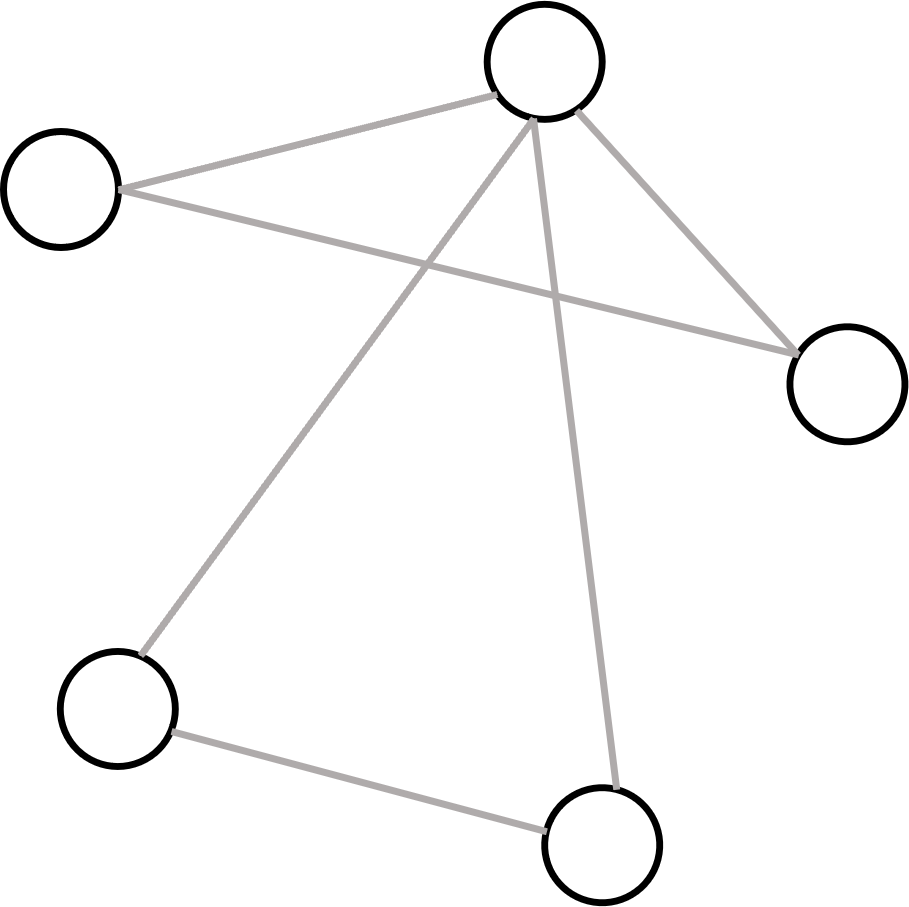
\includegraphics[scale=.625]{Images/graph.png}
    \end{figure}
\end{frame}

%------------------------------------------------
\begin{frame}{What is a Graph?}
    \only<1>{
    \begin{figure}
        \centering
        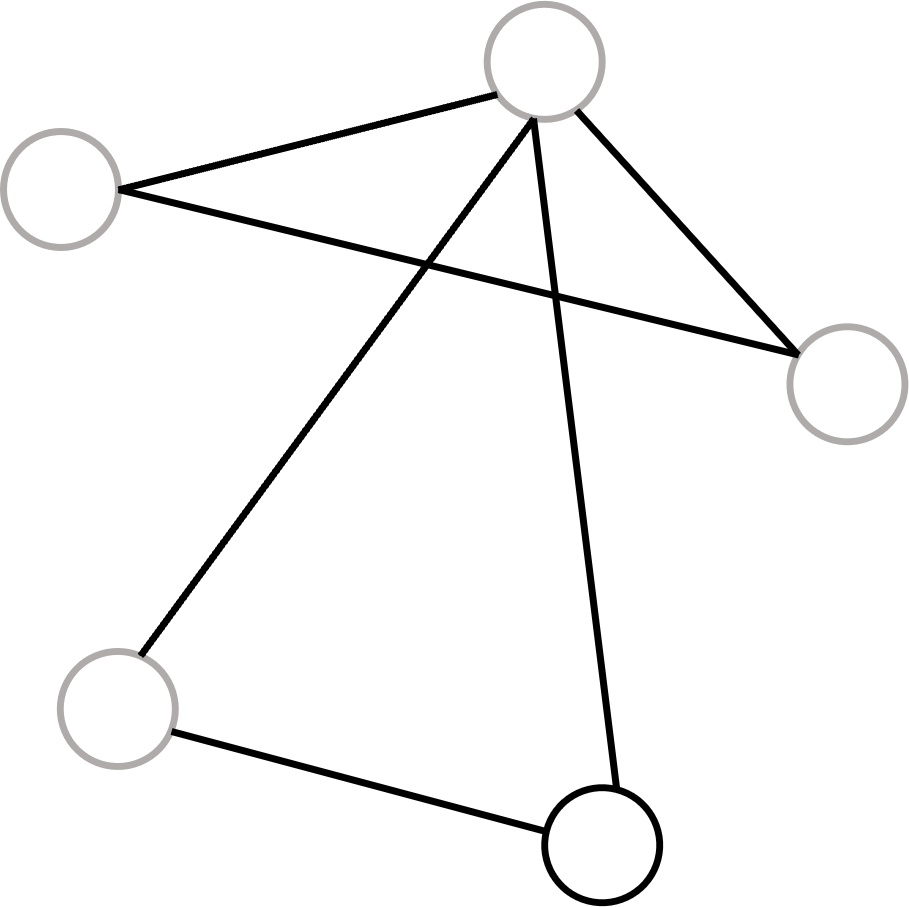
\includegraphics[scale=.625]{Images/undirected-graph.png}
    \end{figure}
    }

    \only<2>{
    \begin{figure}
        \centering
        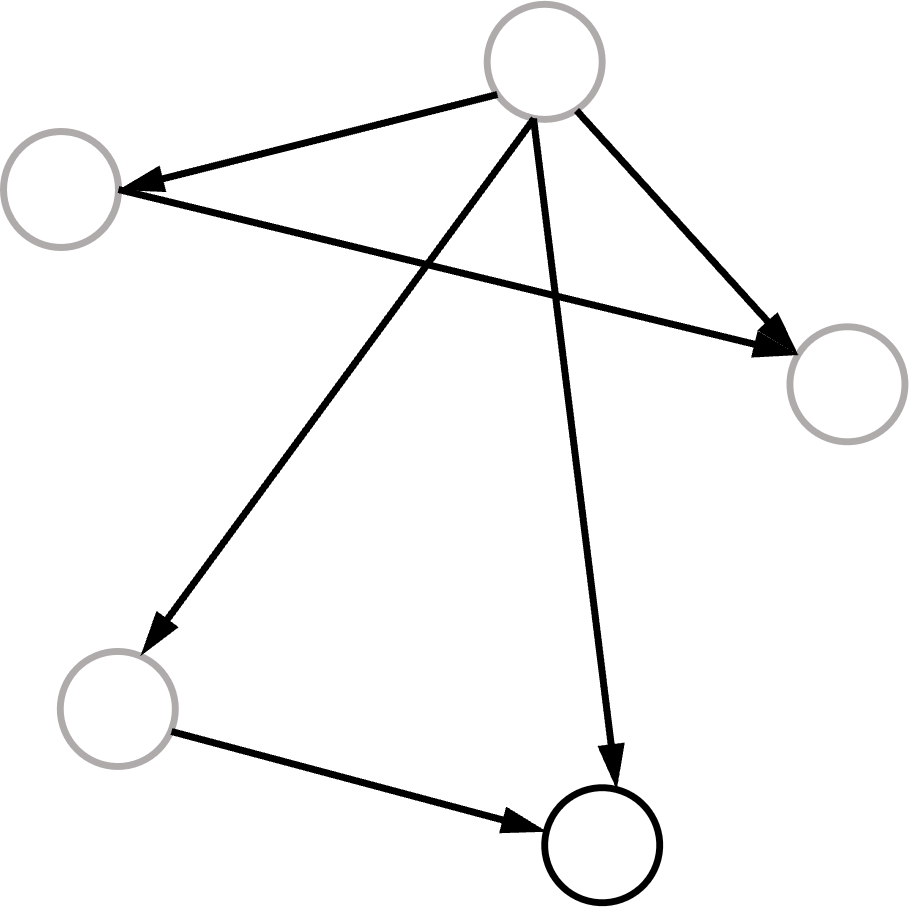
\includegraphics[scale=.625]{Images/directed-graph.png}
    \end{figure}
    }

    \only<3>{
    \begin{figure}
        \centering
        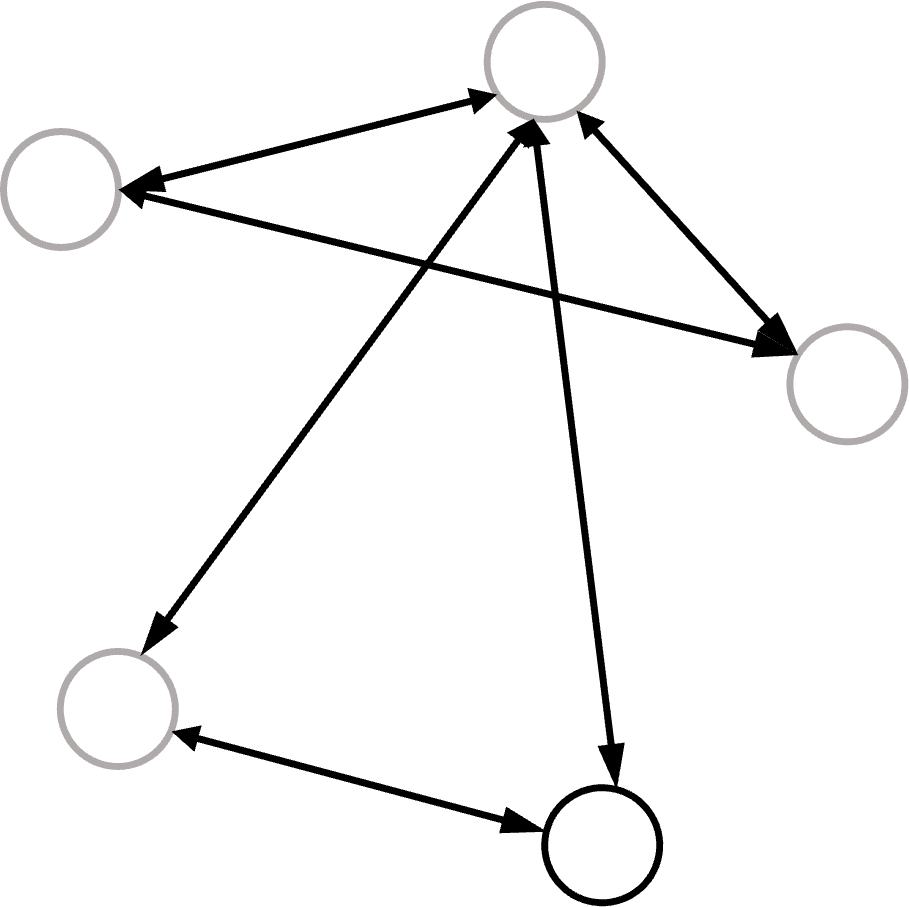
\includegraphics[scale=.625]{Images/bi-directed-graph.png}
    \end{figure}
    }
\end{frame}

%------------------------------------------------
\begin{frame}{Attributes of Graph}
    \centering

    \only<1>{
    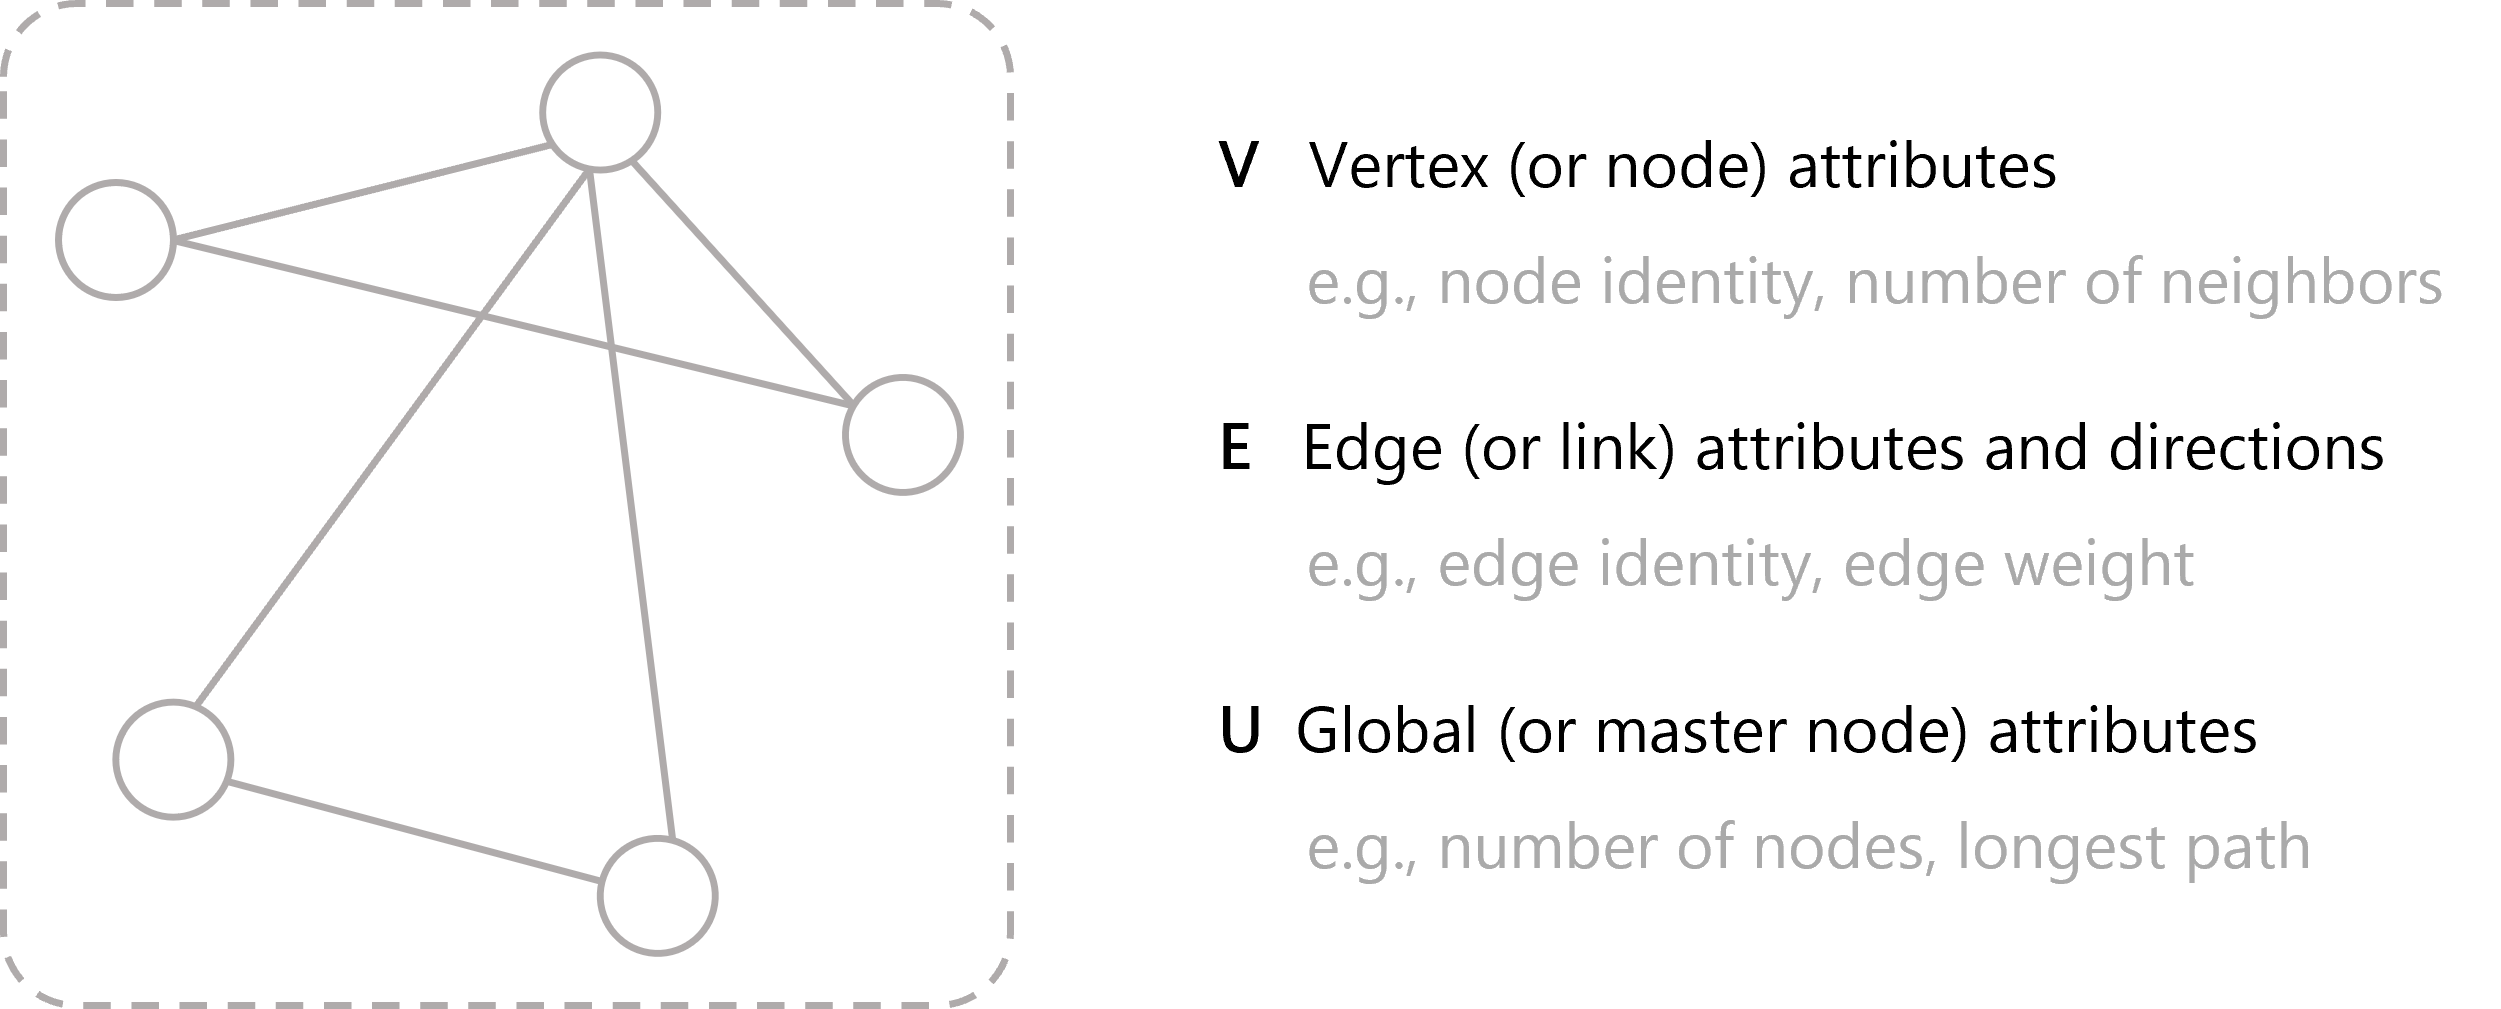
\includegraphics[width=.8\textwidth]{Images/temp-graph.png}
    }
    
    \only<2>{
    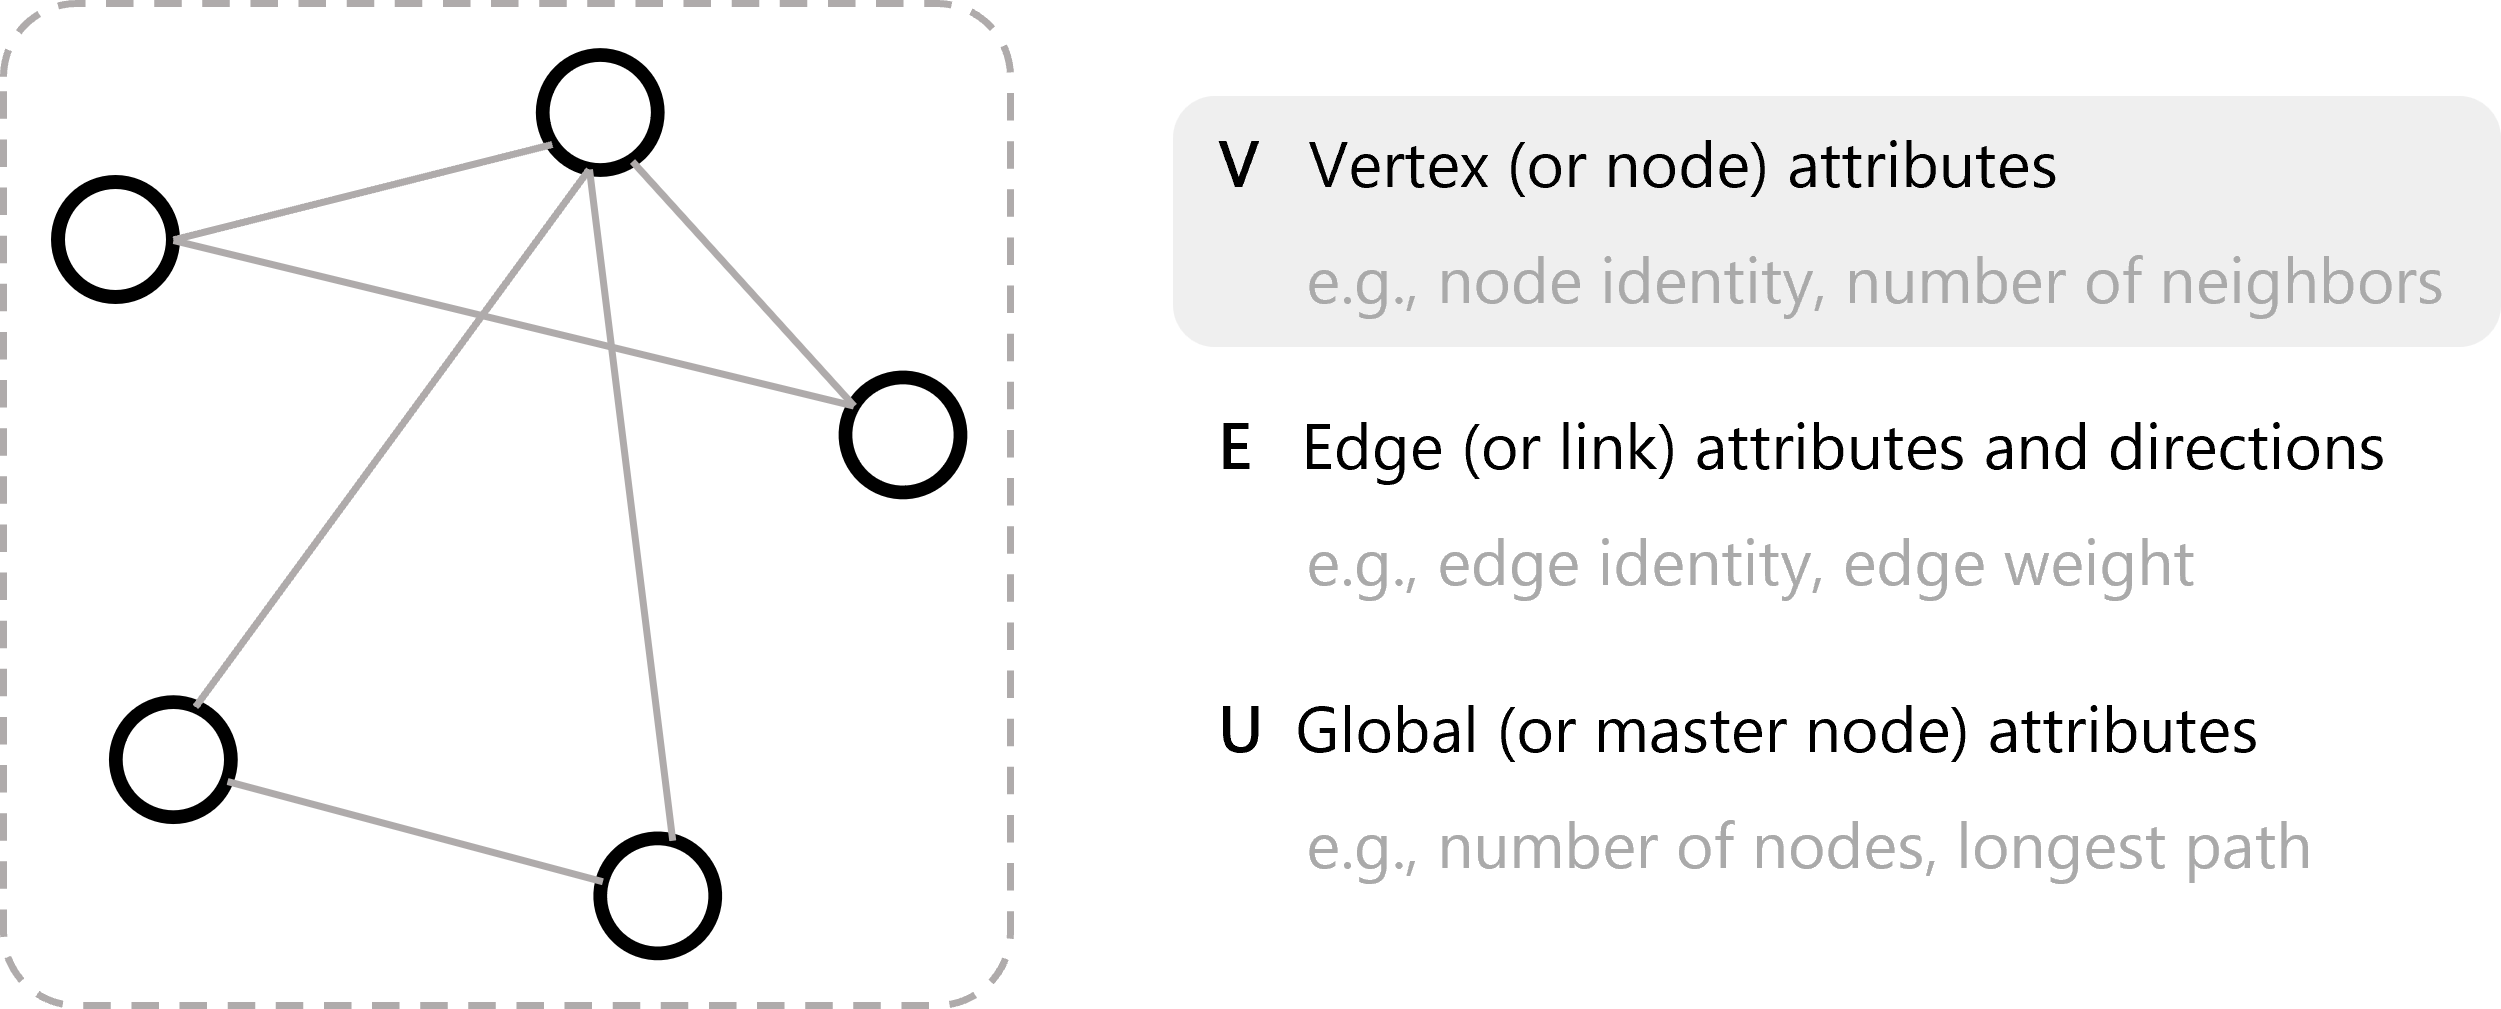
\includegraphics[width=.8\textwidth]{Images/vertex-attribute.png}
    }

    \only<3>{
    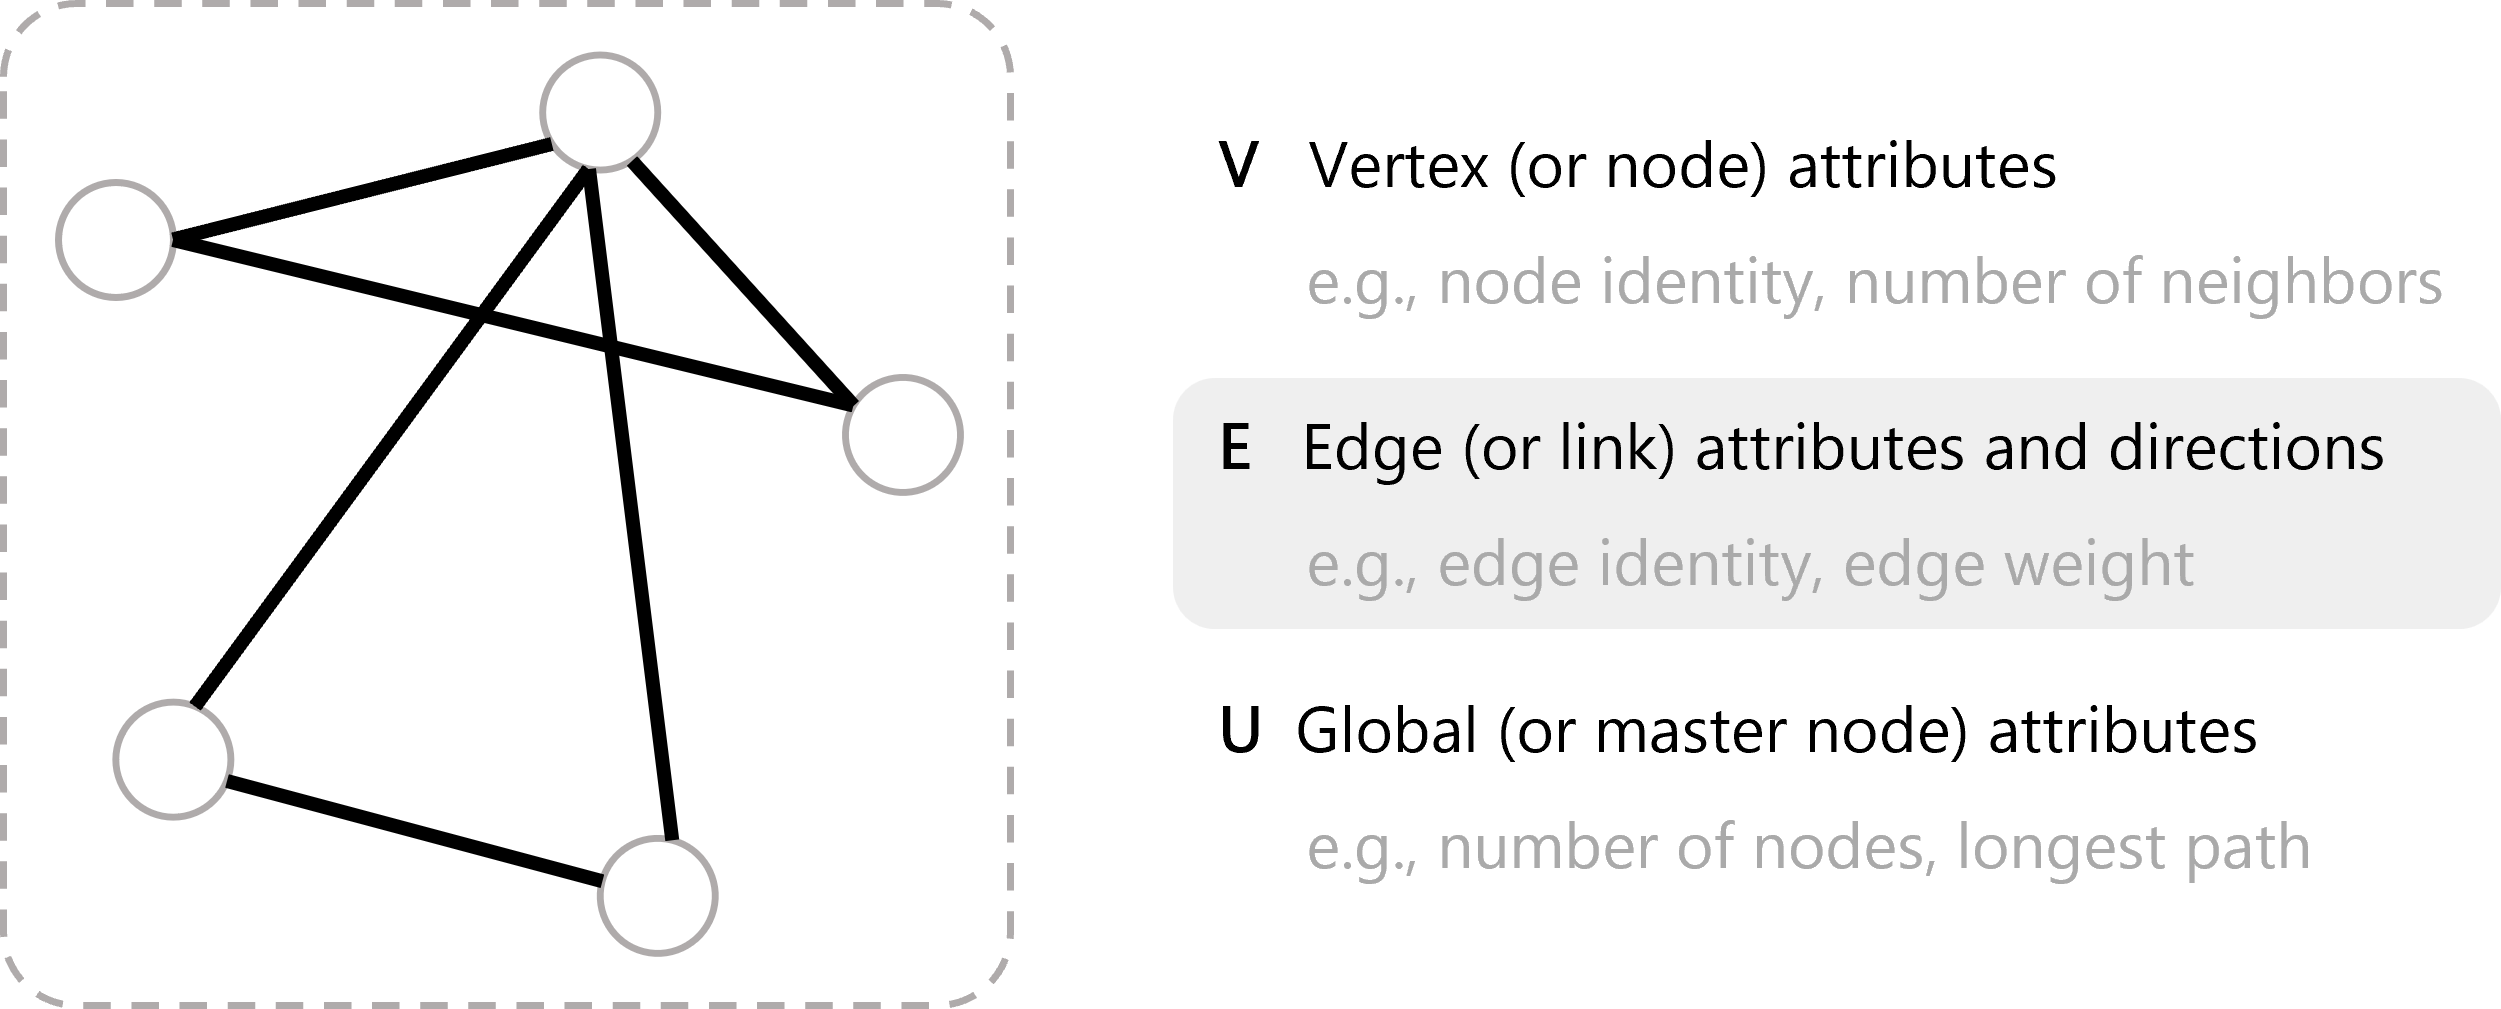
\includegraphics[width=.8\textwidth]{Images/edge-attribute.png}
    }

    \only<4>{
    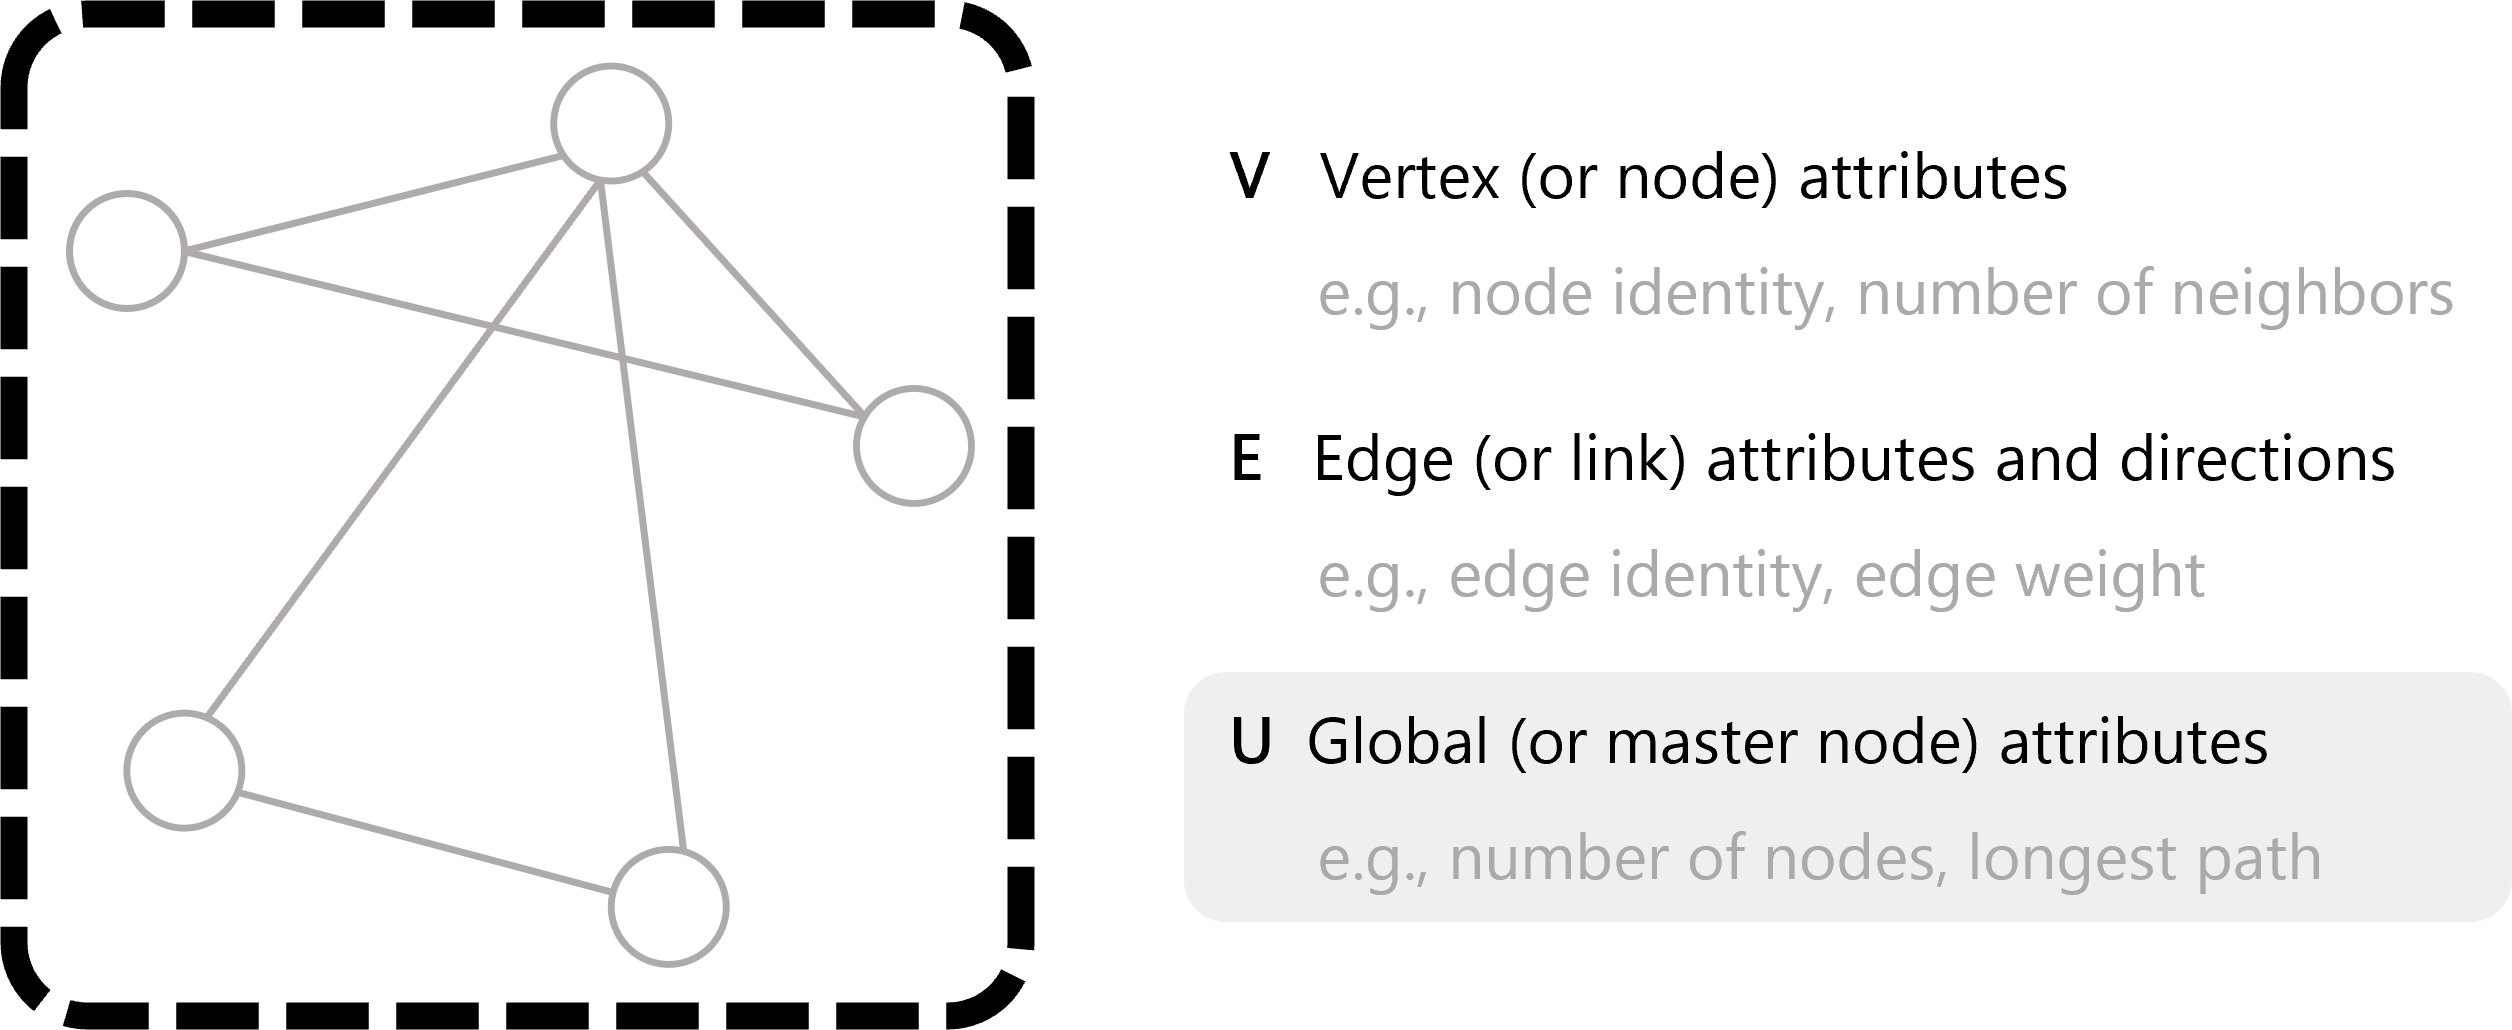
\includegraphics[width=.8\textwidth]{Images/global-attribute.png}
    }
\end{frame}

%------------------------------------------------
\begin{frame}{Attributes of Graph}
    \centering

    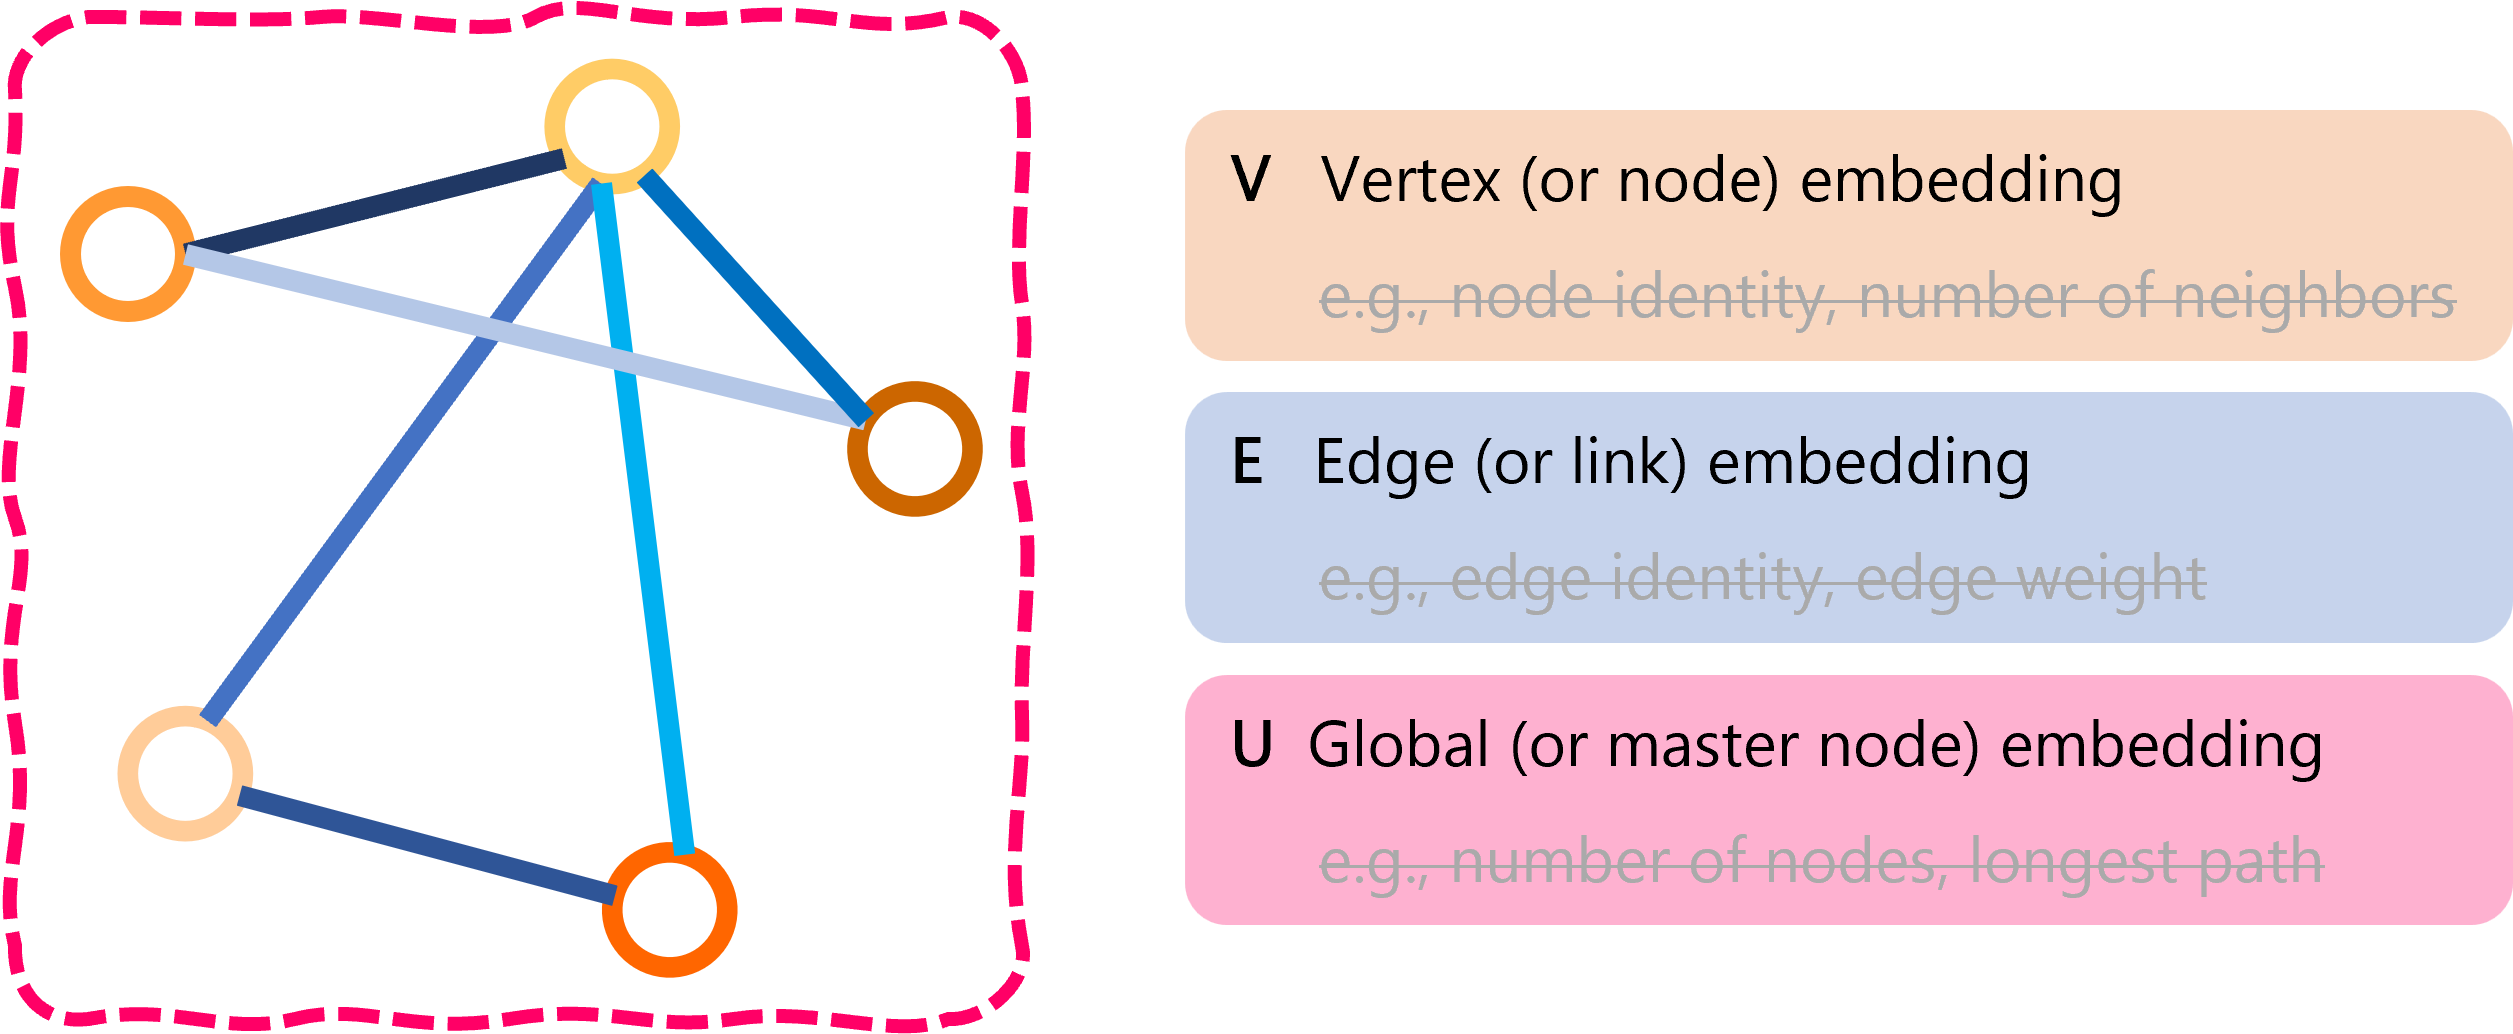
\includegraphics[width=.8\textwidth]{Images/embedding-attributes.png}
\end{frame}

%------------------------------------------------
\subsection{Where to Find them?}
\begin{frame}{}
    \begin{itemize}
        \item[] \Large \textbf{Graphs are all around us}; \large real world objects are often defined in terms of their connections to other things.
    \end{itemize}
\end{frame}

%------------------------------------------------
\begin{frame}{Images as Graphs}
    \centering
    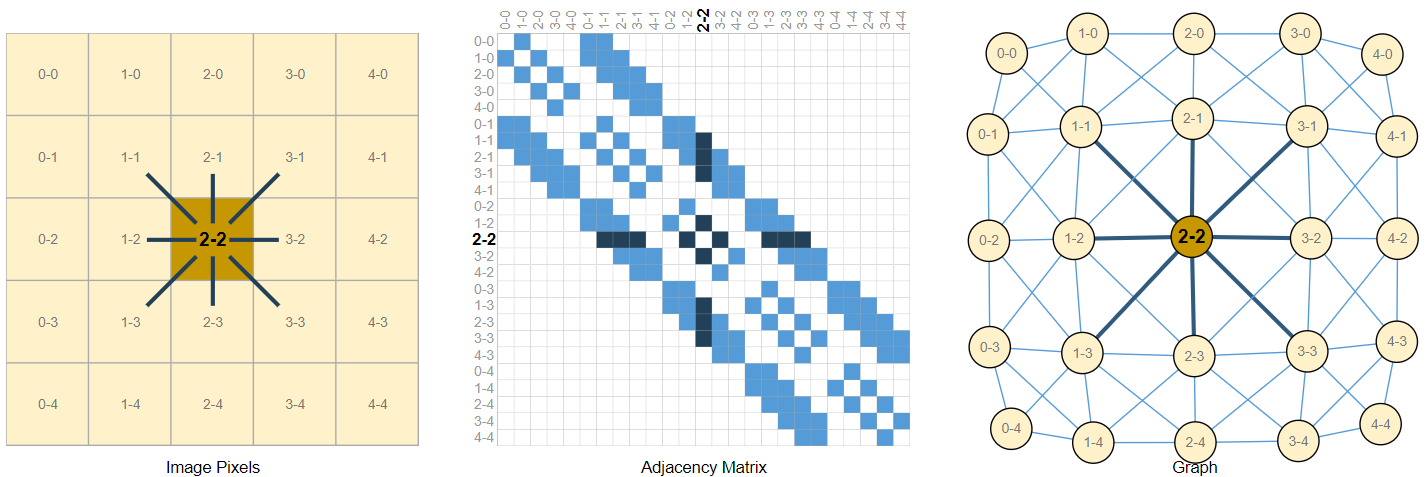
\includegraphics[width=\textwidth]{Images/img2graph.png}
\end{frame}

%------------------------------------------------
\begin{frame}{Text as Graphs}
    \centering
    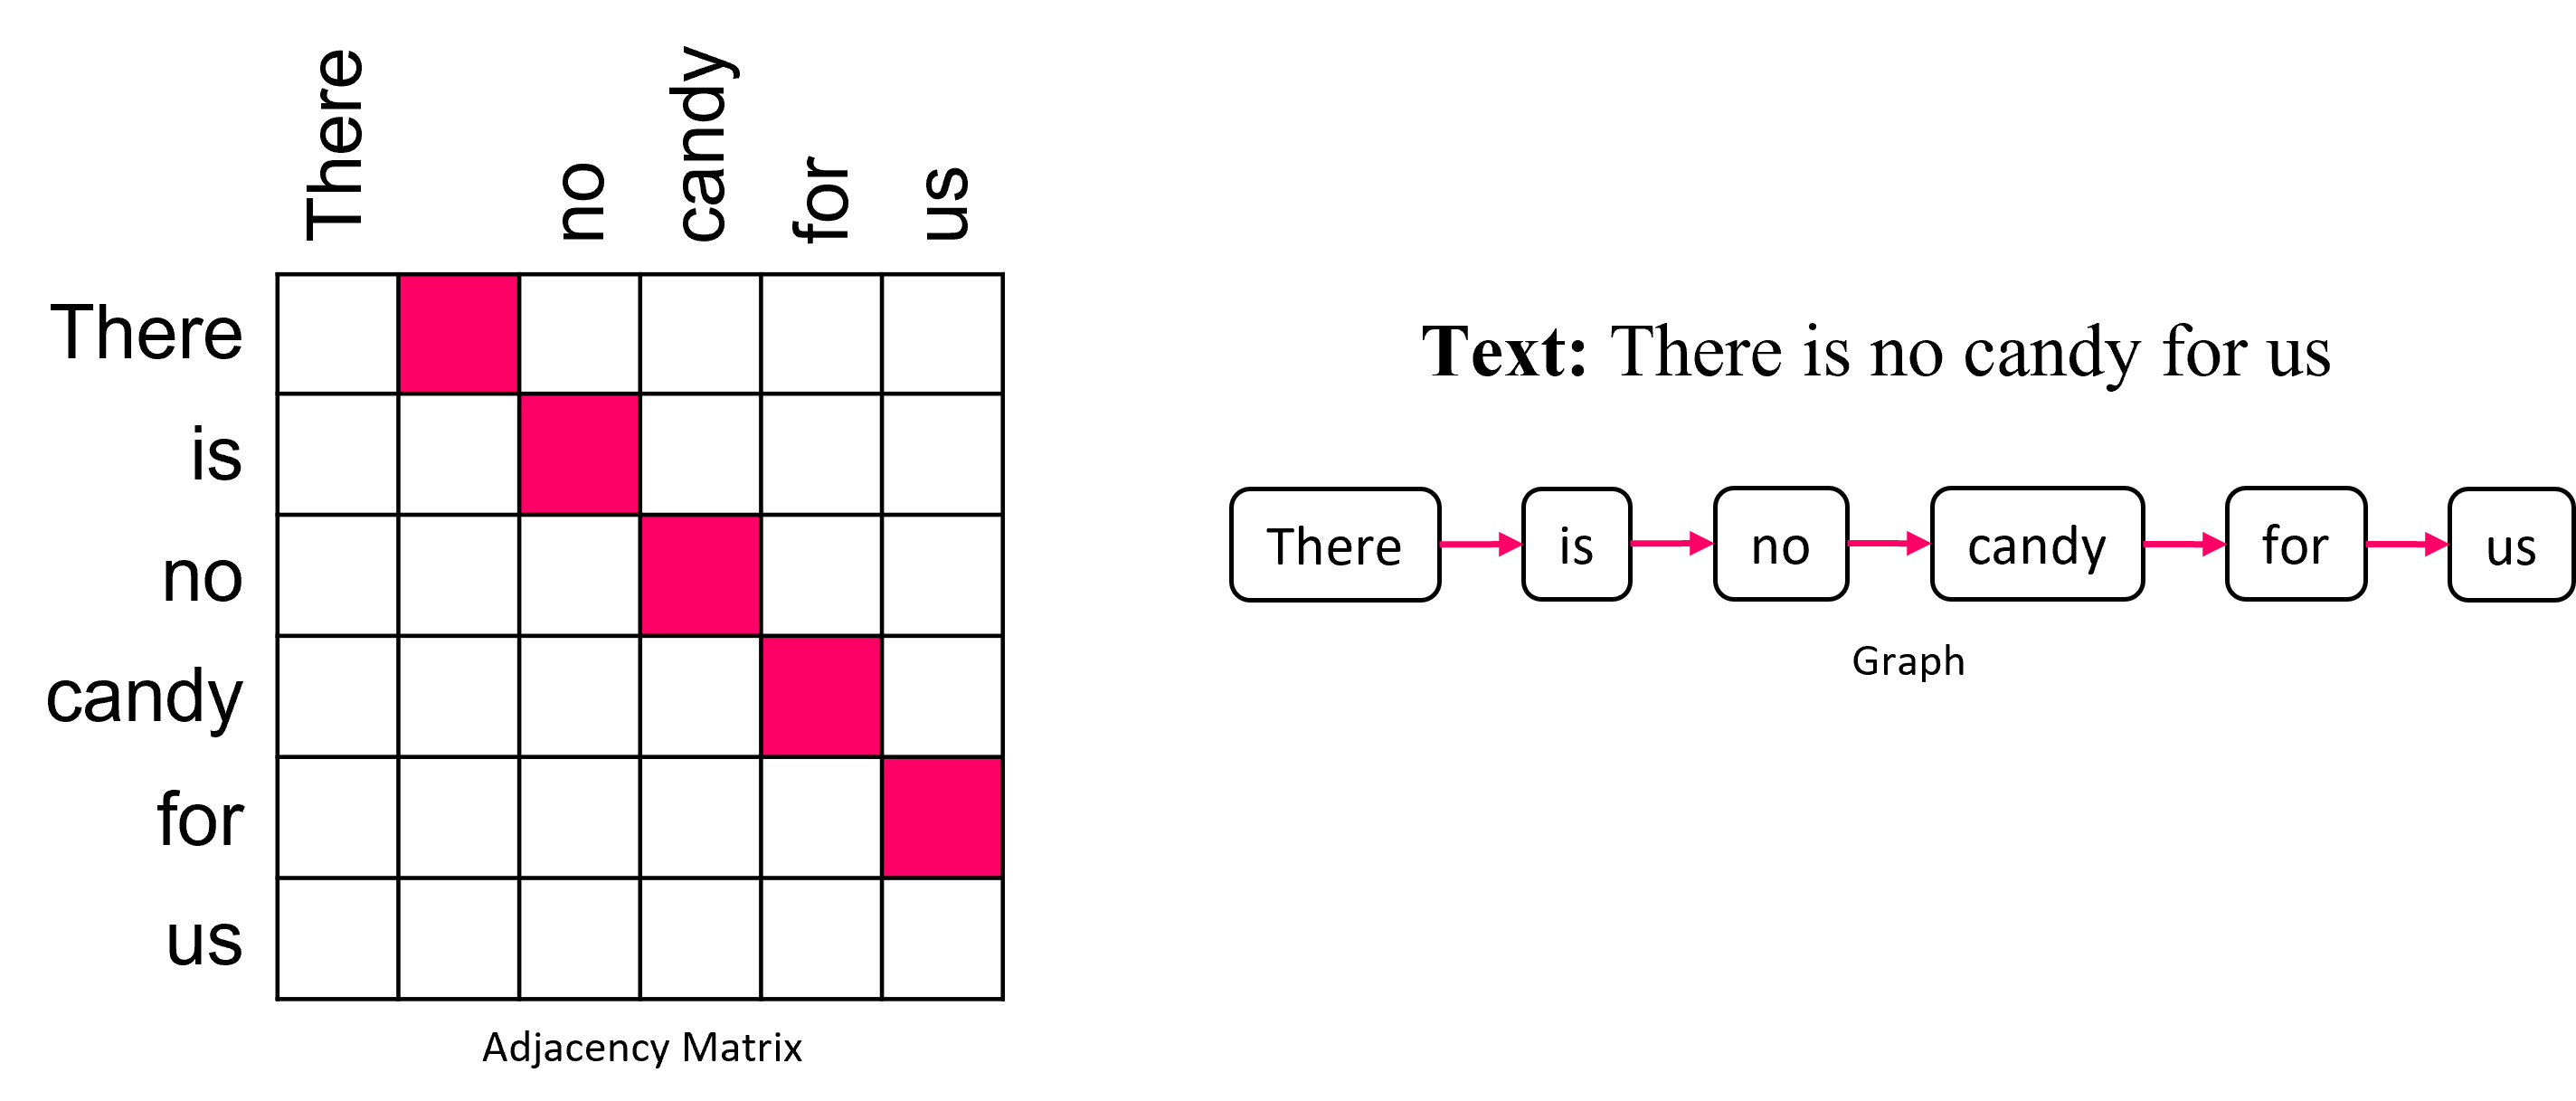
\includegraphics[width=.9\textwidth]{Images/text2graph.png}
\end{frame}

%------------------------------------------------
\begin{frame}{Graph-valued Data in the Wild}
    \begin{columns}[c]
        \begin{column}{.3\textwidth}
            \begin{itemize}[<+->]
                \item Molecules 
                \item Social networks
                \item Citation networks
                \item etc
            \end{itemize}
        \end{column}    

        \begin{column}{.7\textwidth}
            \centering
            \only<1> {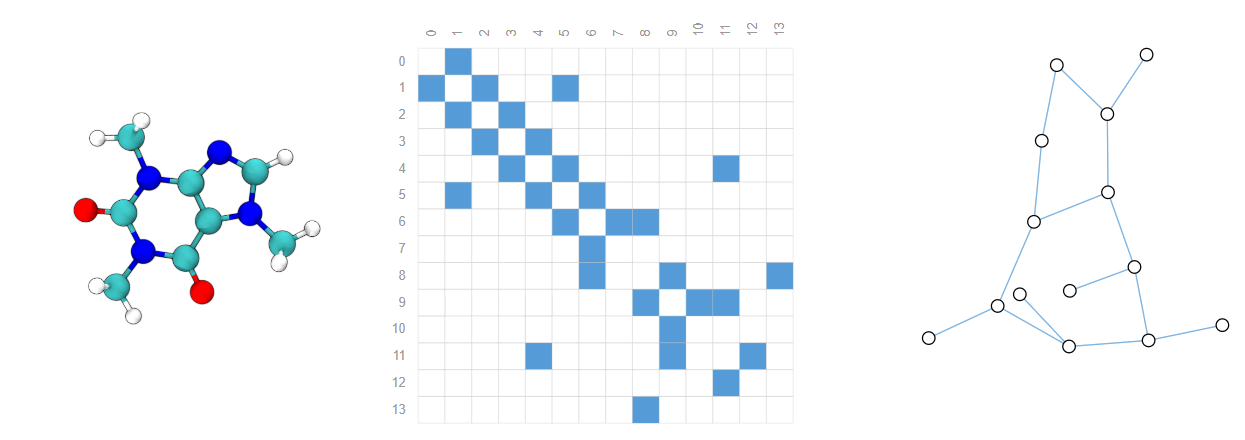
\includegraphics[width=.8\textwidth]{Images/molecules-as-graphs.png}}
            \only<2> {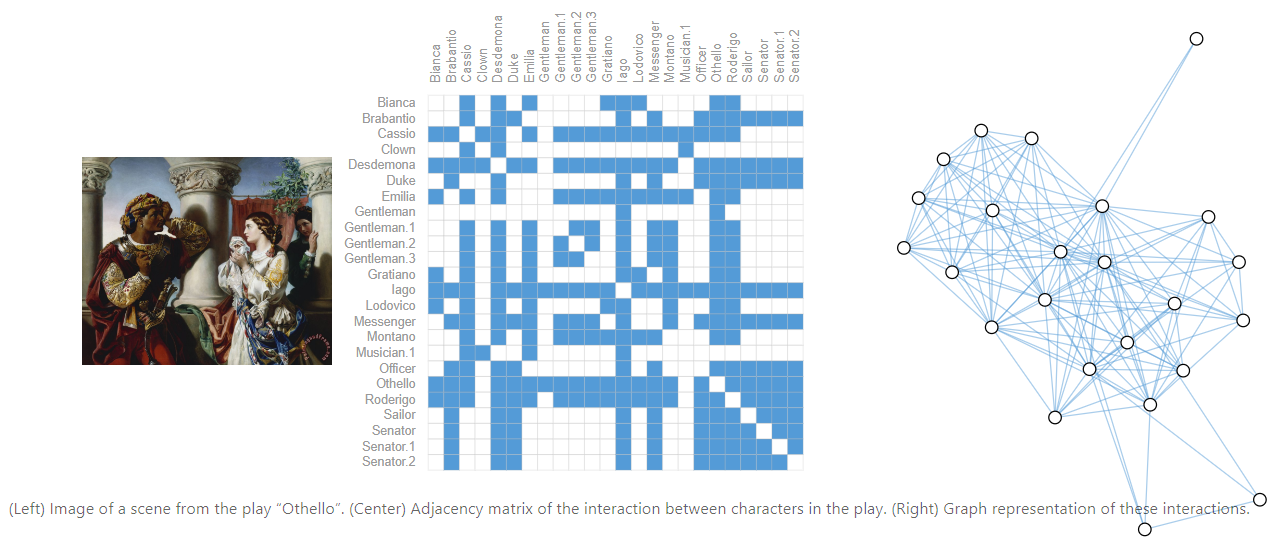
\includegraphics[width=.8\textwidth]{Images/social-networks-as-graphs.png}}
            \only<3> {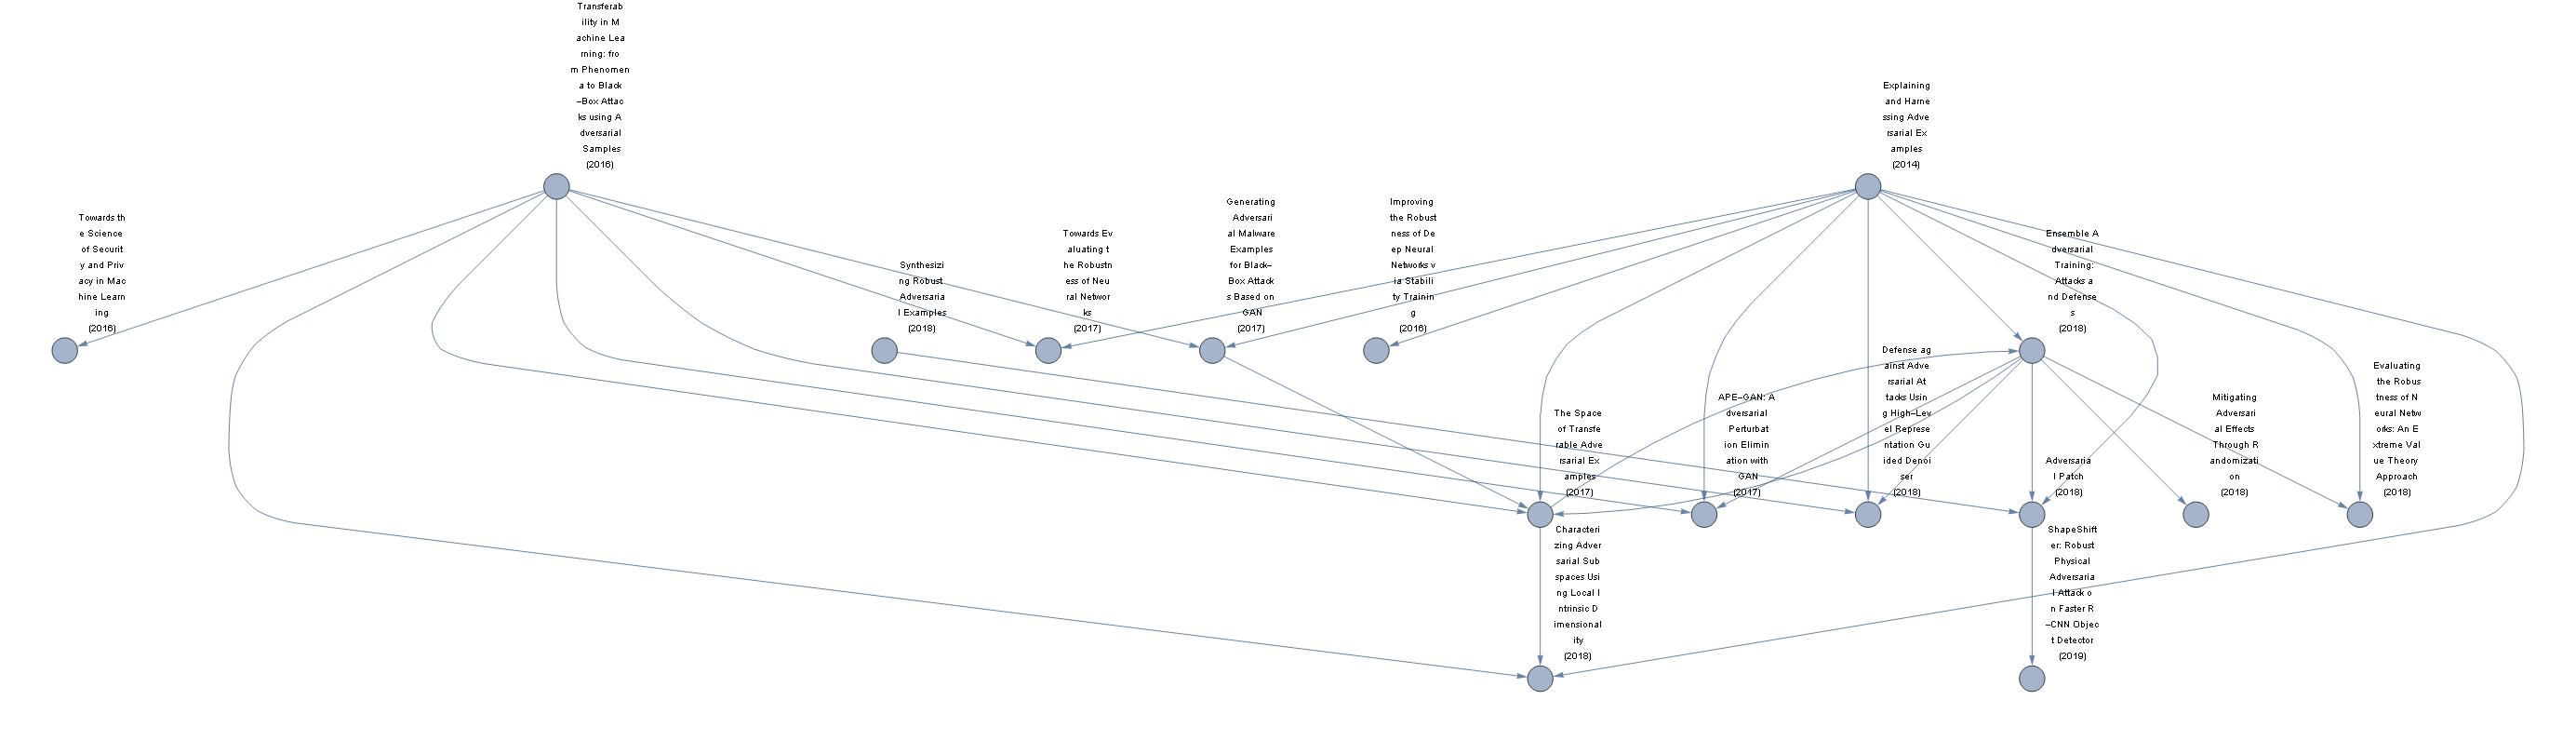
\includegraphics[width=.9\textwidth]{Images/citation-graph.jpg}}
            \only<4> {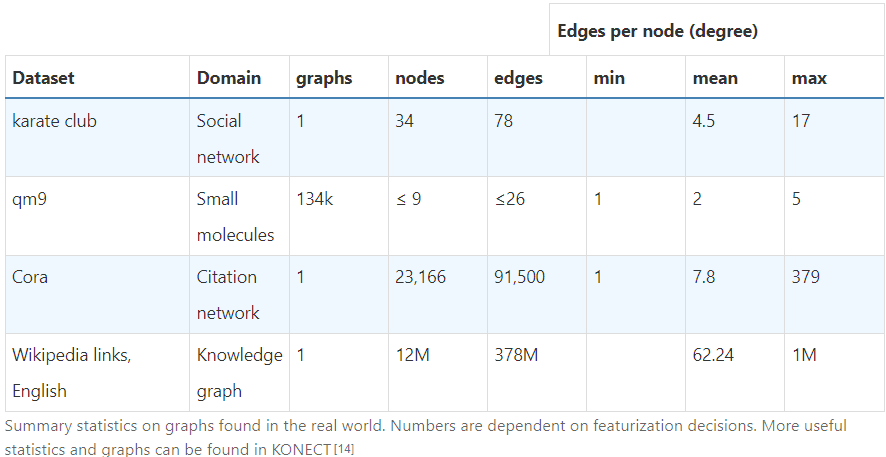
\includegraphics[width=.75\textwidth]{Images/graph-in-the-wild.png}}
        \end{column}
    \end{columns}
\end{frame}

%------------------------------------------------
\subsection{What Tasks to Perform on Graphs?}
\begin{frame}{}
    \centering
    \Large 
    What types of problems have graph structured data?
\end{frame}

%------------------------------------------------
\begin{frame}{Graph-level Task}
    \begin{columns}
        \begin{column}{.56\textwidth}
            \only<4->{\vspace{1.325cm}}
            \begin{itemize}
                \item Predicting the property of an entire graph
                \only<4->{
                \begin{itemize}
                    \item the smell of the molecular
                    \item image classification
                    \item sentiment analysis of text 
                \end{itemize}}
            \end{itemize}
        \end{column}

        % \vrule
        
        \begin{column}{.44\textwidth}
            \uncover<2->{
            \begin{itemize}
                \uncover<2->{\item \textbf{Input}: graphs}
                \uncover<3->{\item \textbf{Output}: labels for each graph}
            \end{itemize}}
        \end{column}
    \end{columns}

    \only<2>{
    \begin{figure}
        \centering
        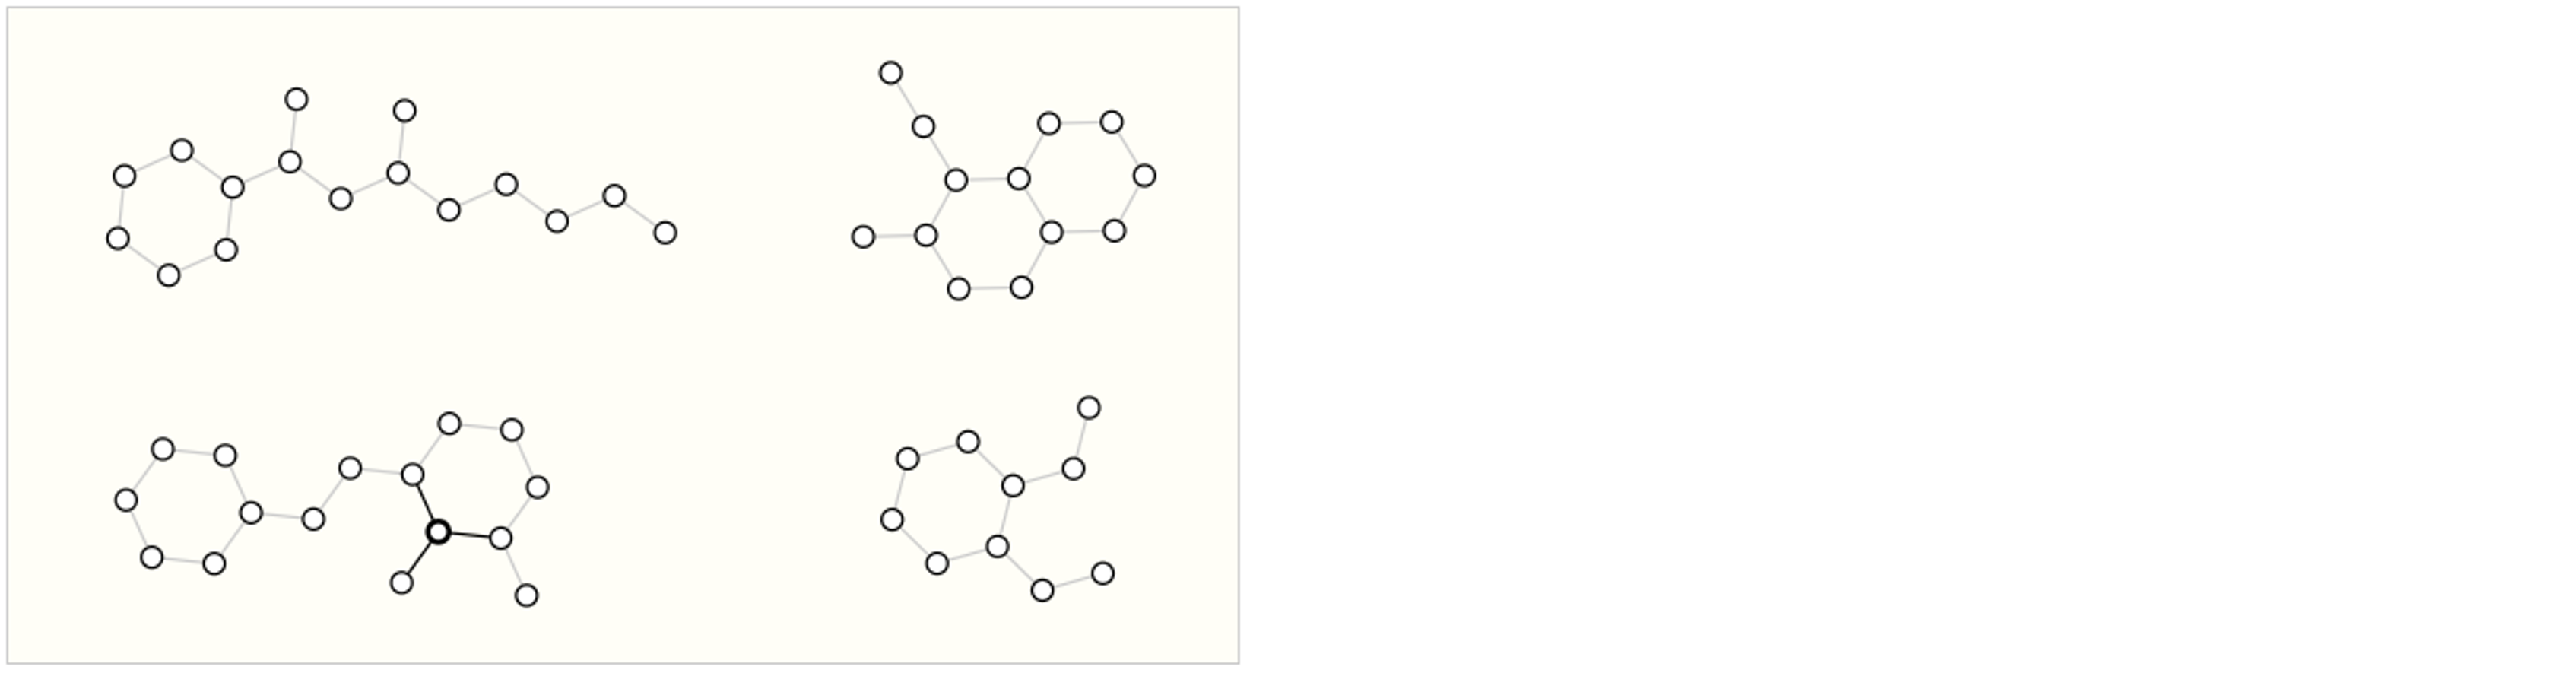
\includegraphics[width=.8\textwidth]{Images/graph-prediction-input.png}
    \end{figure}}

    \only<3>{\begin{figure}
        \centering
        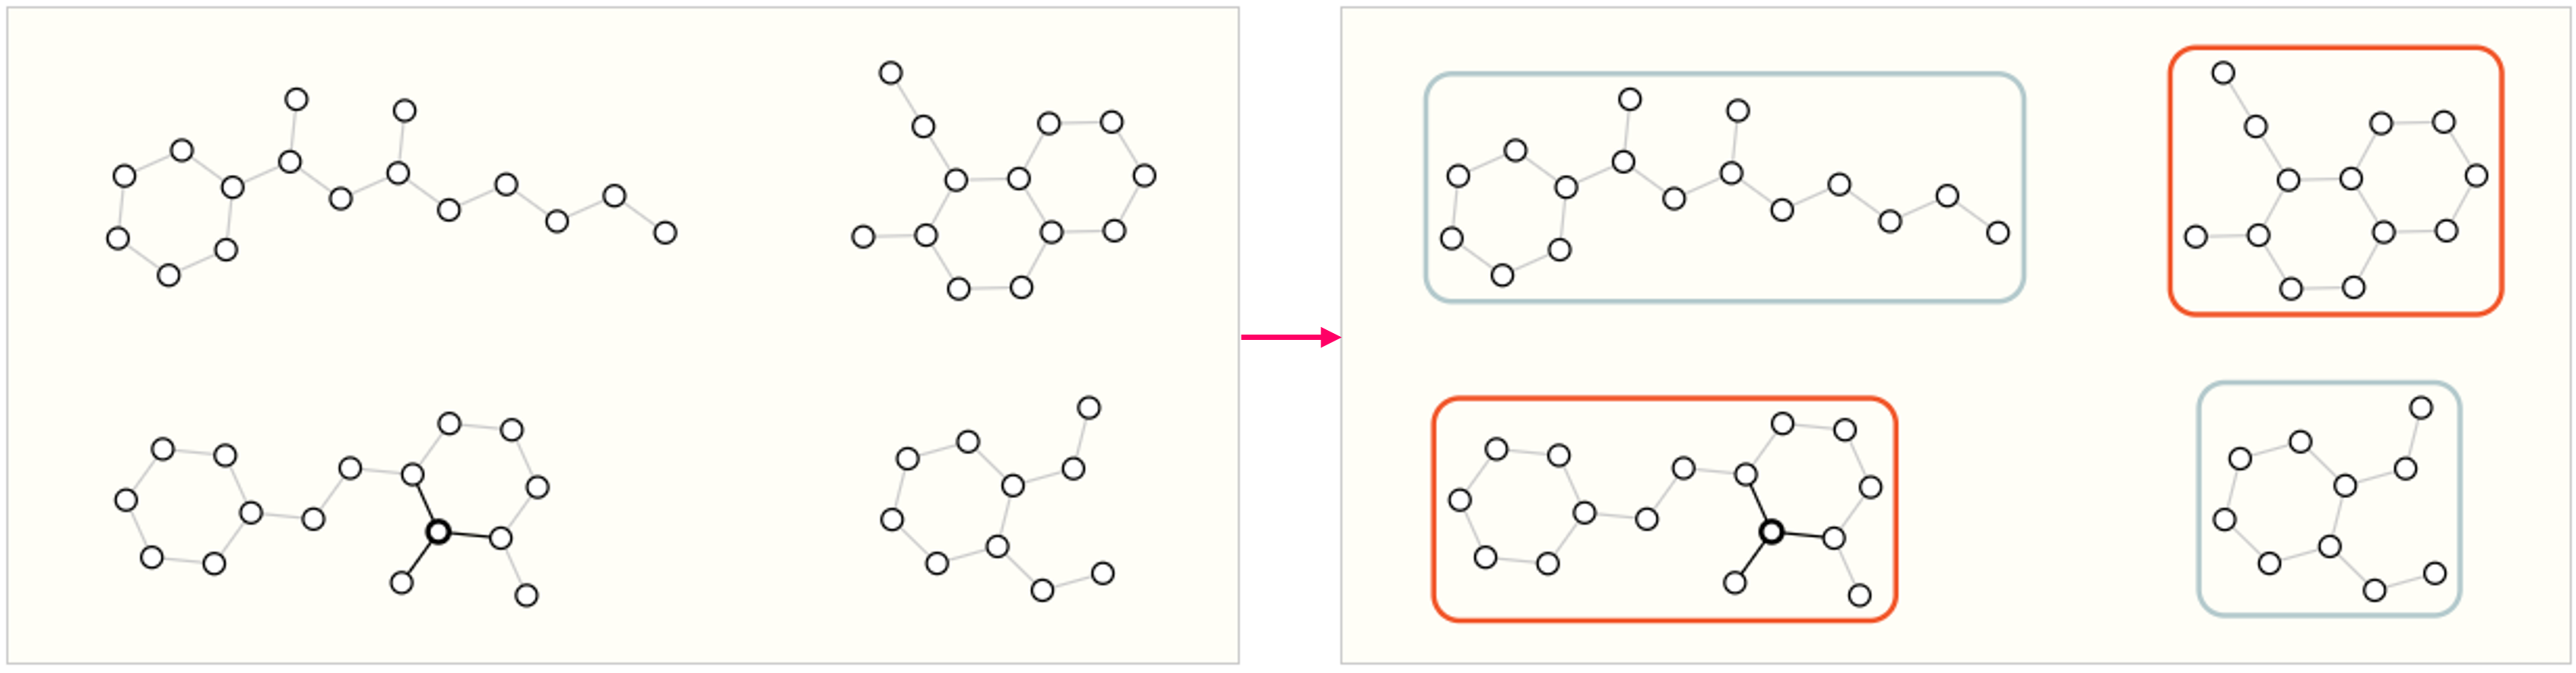
\includegraphics[width=.8\textwidth]{Images/graph-prediction-input-output.png}
    \end{figure}}

    \only<1>{
    \begin{figure}
        \centering
        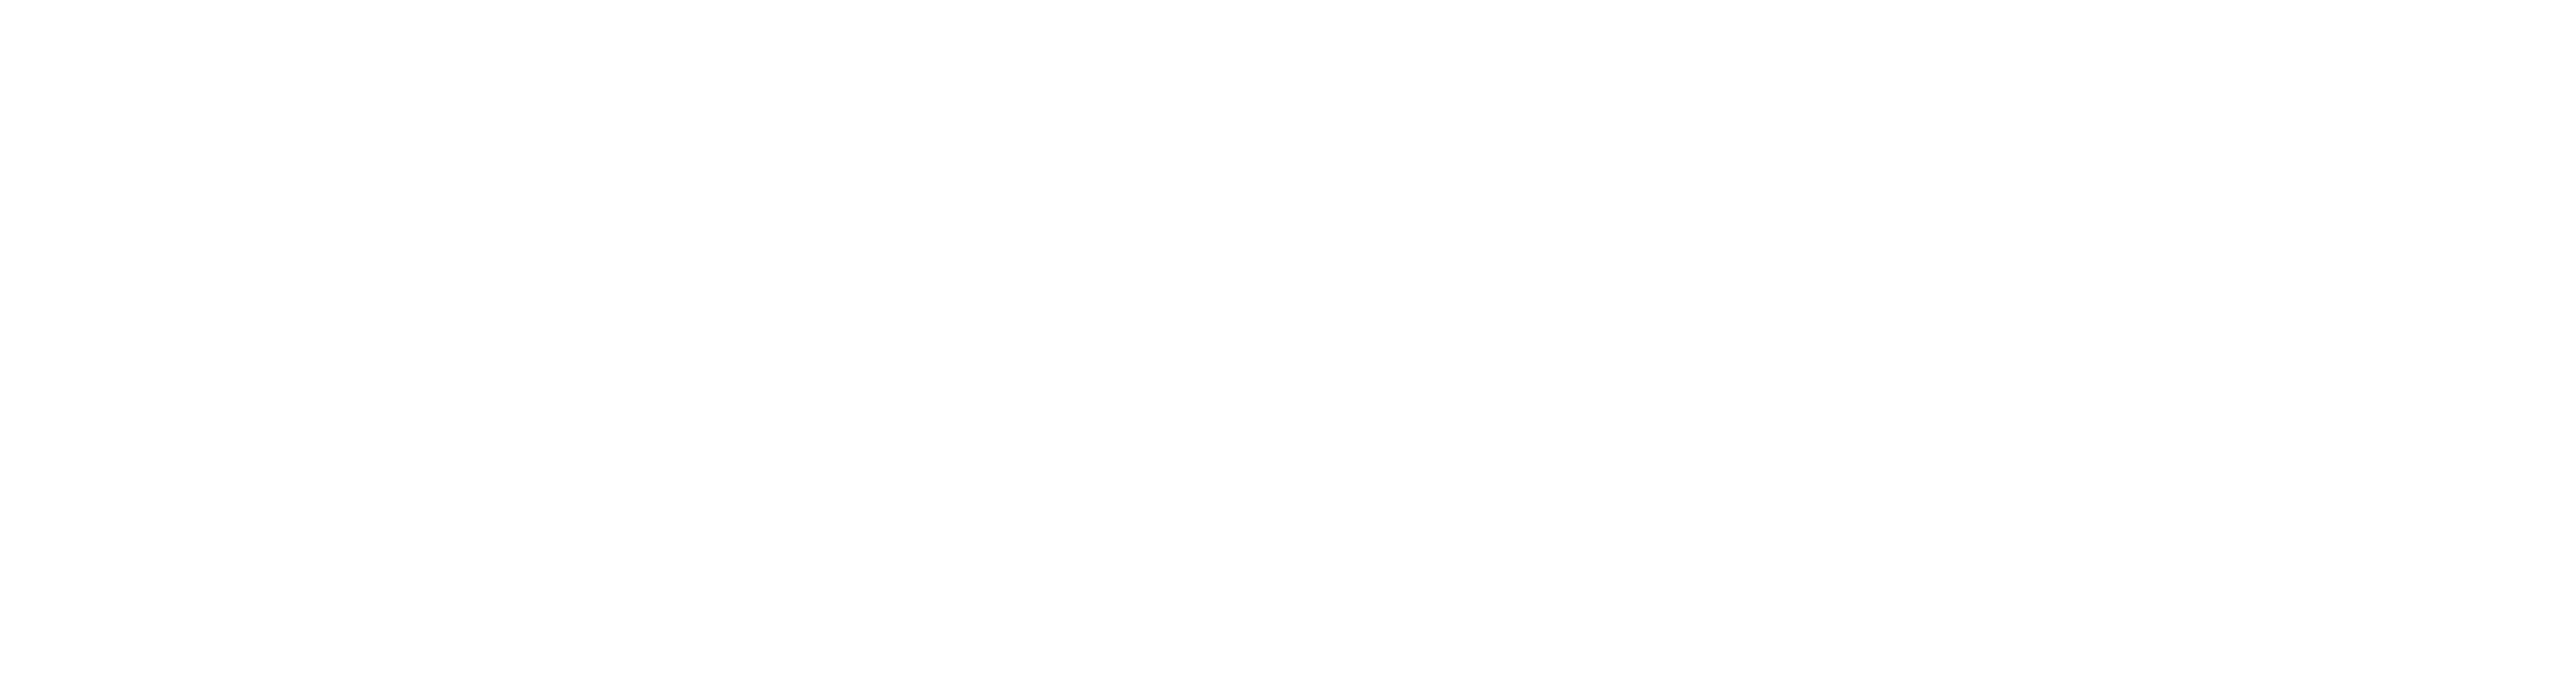
\includegraphics[width=.8\textwidth]{Images/graph-prediction-wh.png}
    \end{figure}
    }
\end{frame}

%------------------------------------------------
\begin{frame}{Node-level Task}
    \begin{columns}
        \begin{column}{.56\textwidth}
        \only<4->{\vspace{1.325cm}}
            \begin{itemize}
                \item Predicting the identity or role of each node 
                \only<4->{
                \begin{itemize}
                    \item image segmentation
                    \item PoS of each word
                \end{itemize}}
            \end{itemize}
        \end{column}

        % \vrule
        
        \begin{column}{.44\textwidth}
            \uncover<2->{
            \begin{itemize}
                \uncover<2->{\item \textbf{Input}: graphs (unlabeled nodes)}
                \uncover<3->{\item \textbf{Output}: graph node labels}
            \end{itemize}}
        \end{column}
    \end{columns}

    \only<2>{
    \begin{figure}
        \centering
        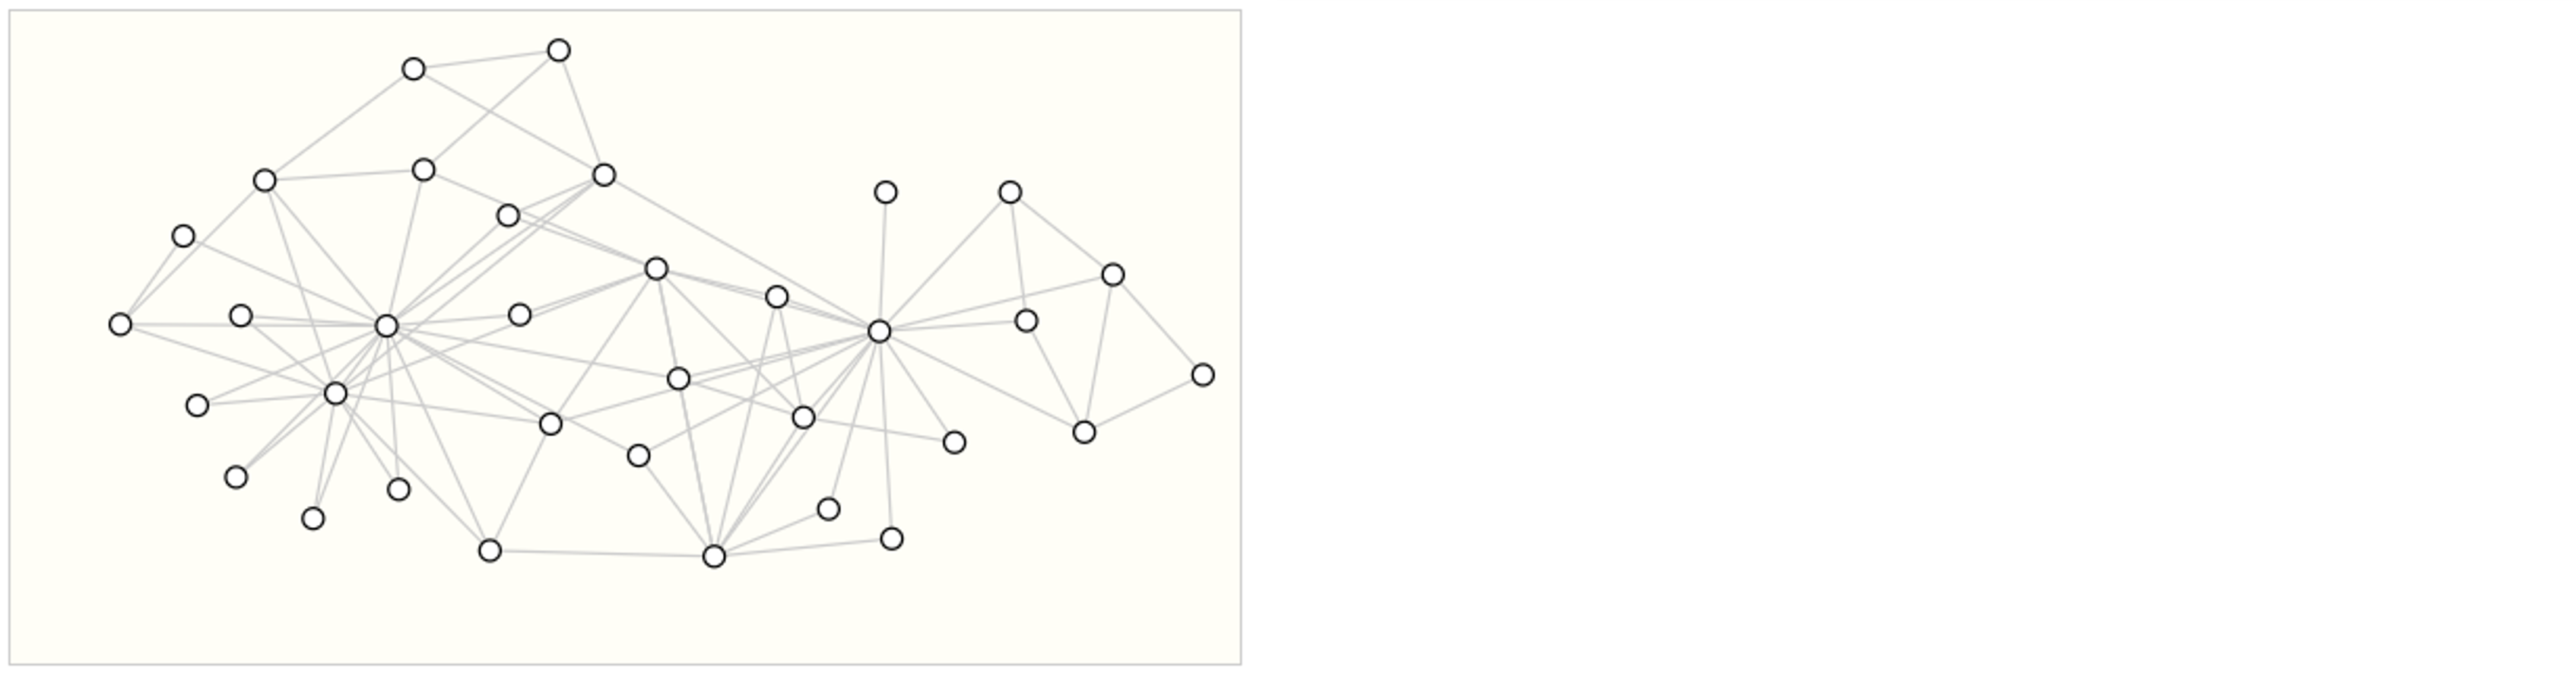
\includegraphics[width=.8\textwidth]{Images/node-prediction-input.png}
    \end{figure}}

    \only<3>{\begin{figure}
        \centering
        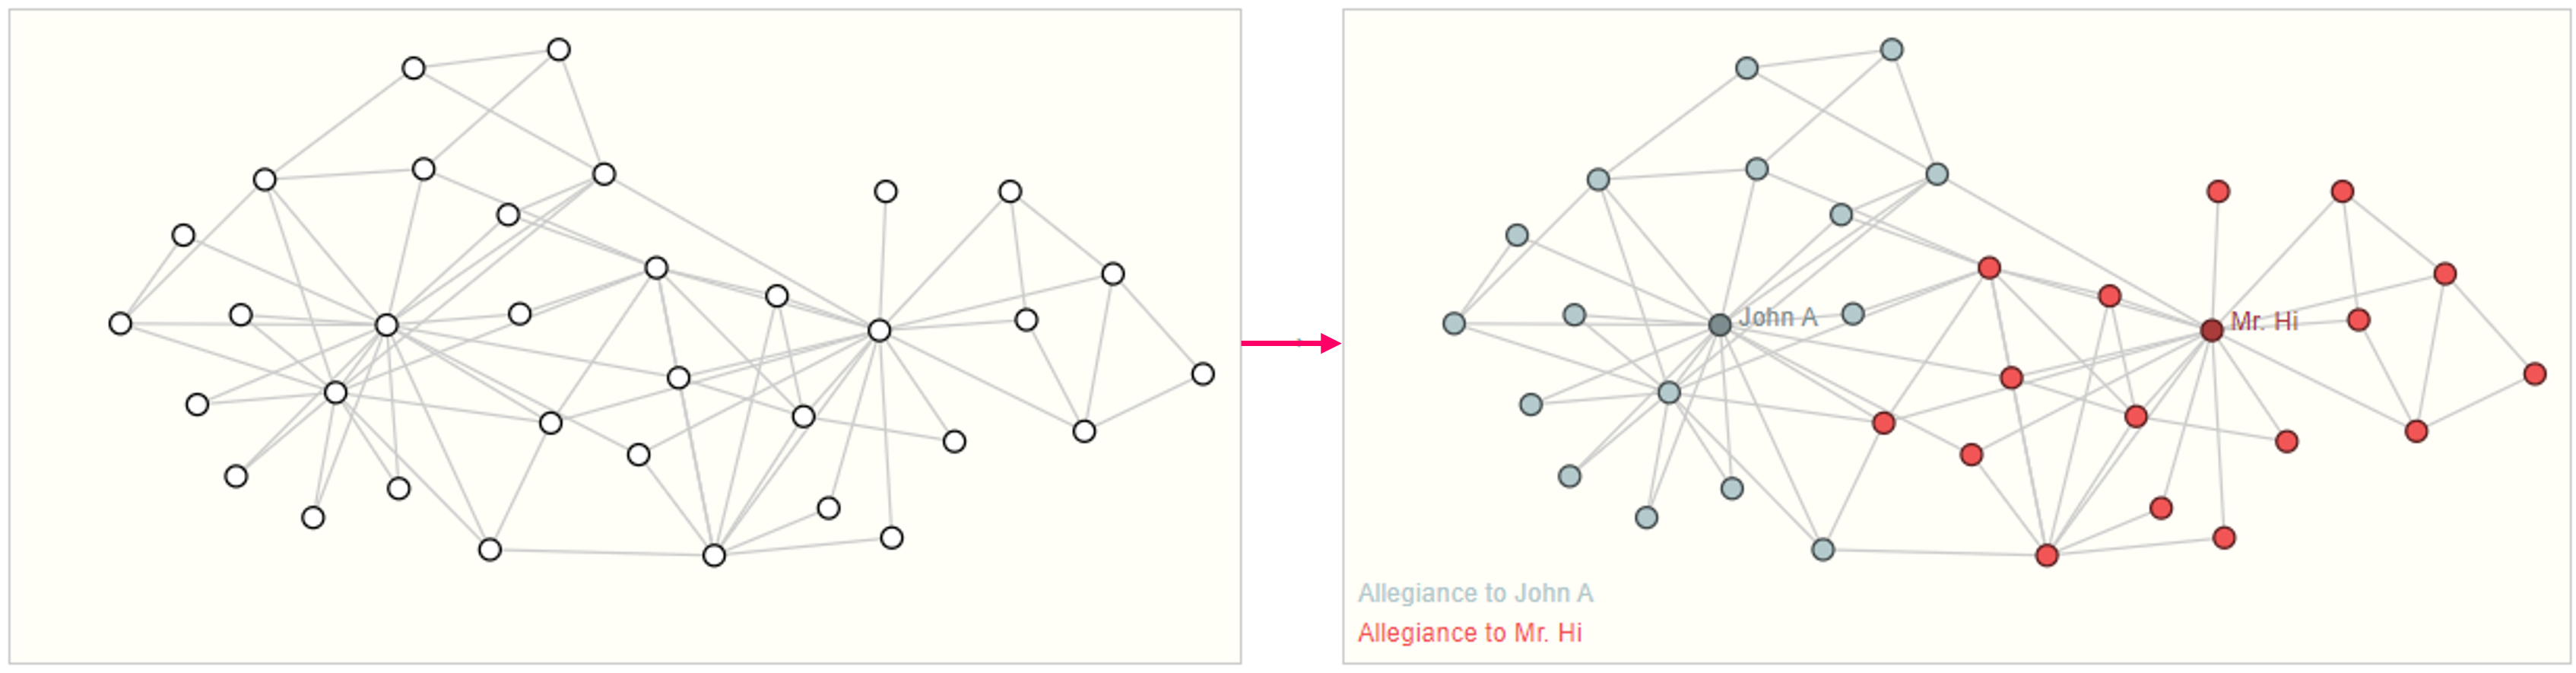
\includegraphics[width=.8\textwidth]{Images/node-prediction-input-output.png}
    \end{figure}}

    \only<1>{
    \begin{figure}
        \centering
        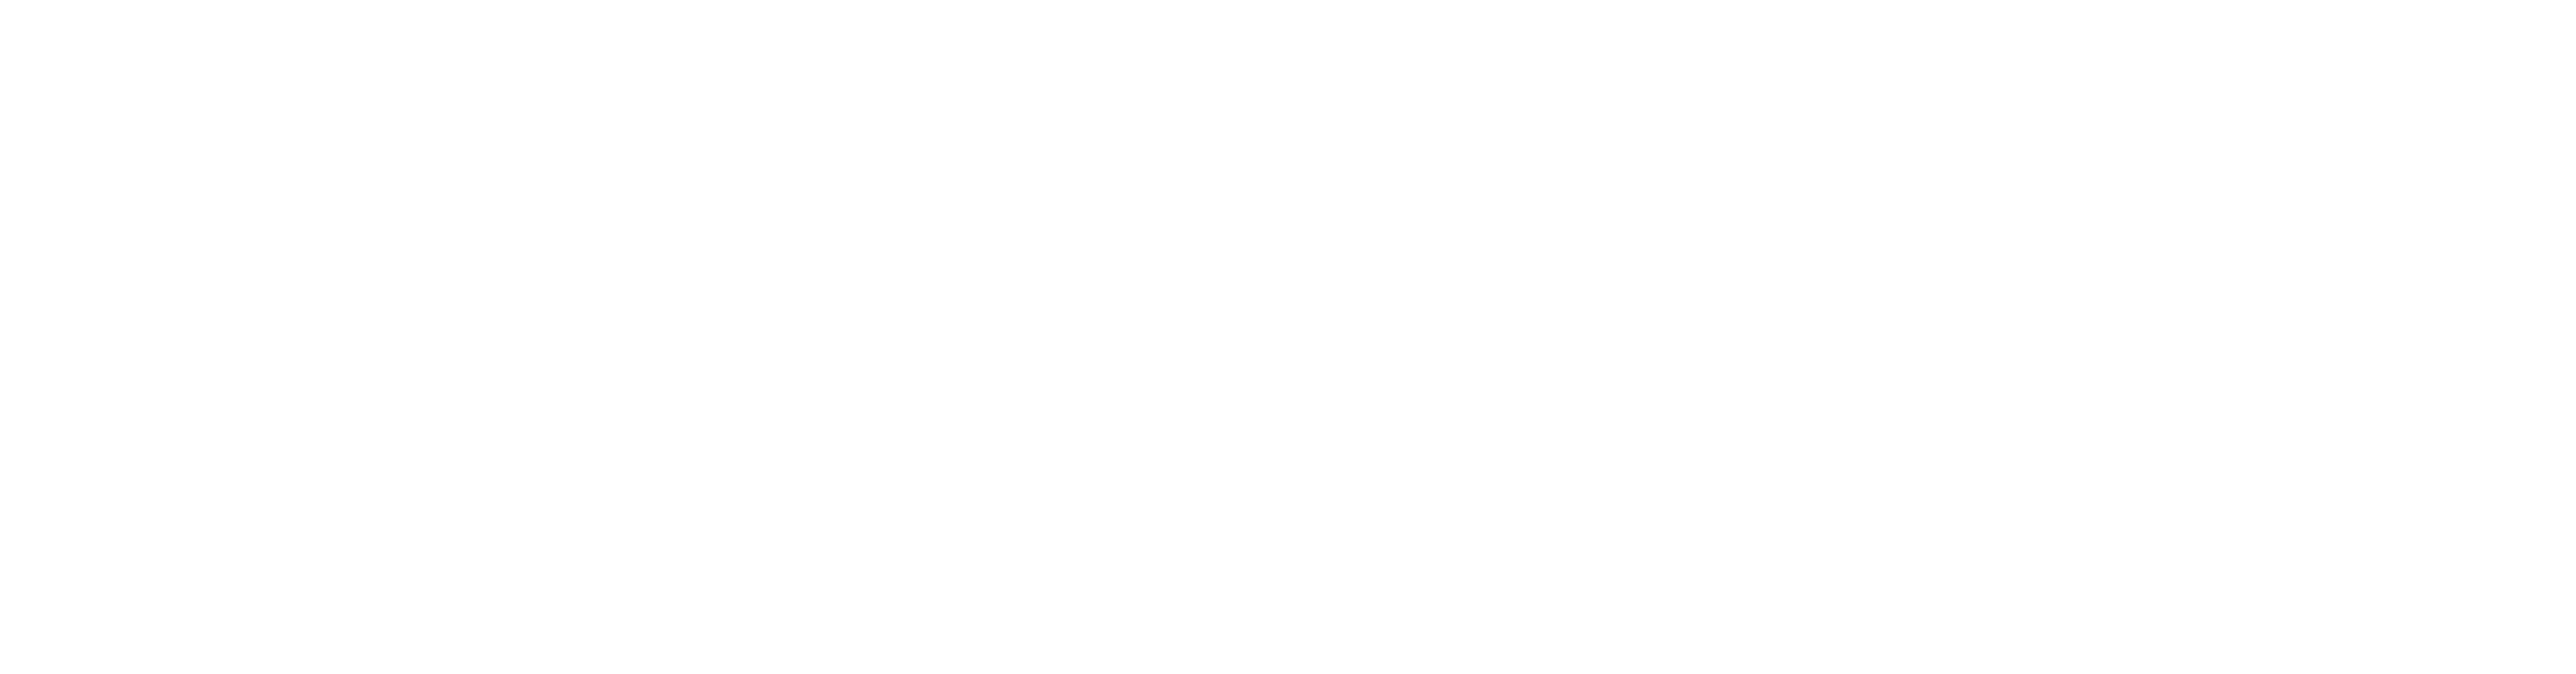
\includegraphics[width=.8\textwidth]{Images/node-prediction-h.png}
    \end{figure}
    }
\end{frame}

%------------------------------------------------
\begin{frame}{Edge-level Task}
    \only<1-4>{
    \begin{columns}
    \only<4->{\vspace{1.325cm}}
        \begin{column}{.56\textwidth}
            \begin{itemize}
                \item Predicting the identity or role of each edge
                \only<4->{
                \begin{itemize}
                    \item scence understanding
                \end{itemize}}
            \end{itemize}
        \end{column}

        % \vrule
        
        \begin{column}{.44\textwidth}
            \uncover<2->{
            \begin{itemize}
                \uncover<2->{\item \textbf{Input}: graphs (unlabeled edges)}
                \uncover<3->{\item \textbf{Output}: labels for edges}
            \end{itemize}}
        \end{column}
    \end{columns}

    \only<2>{
    \begin{figure}
        \centering
        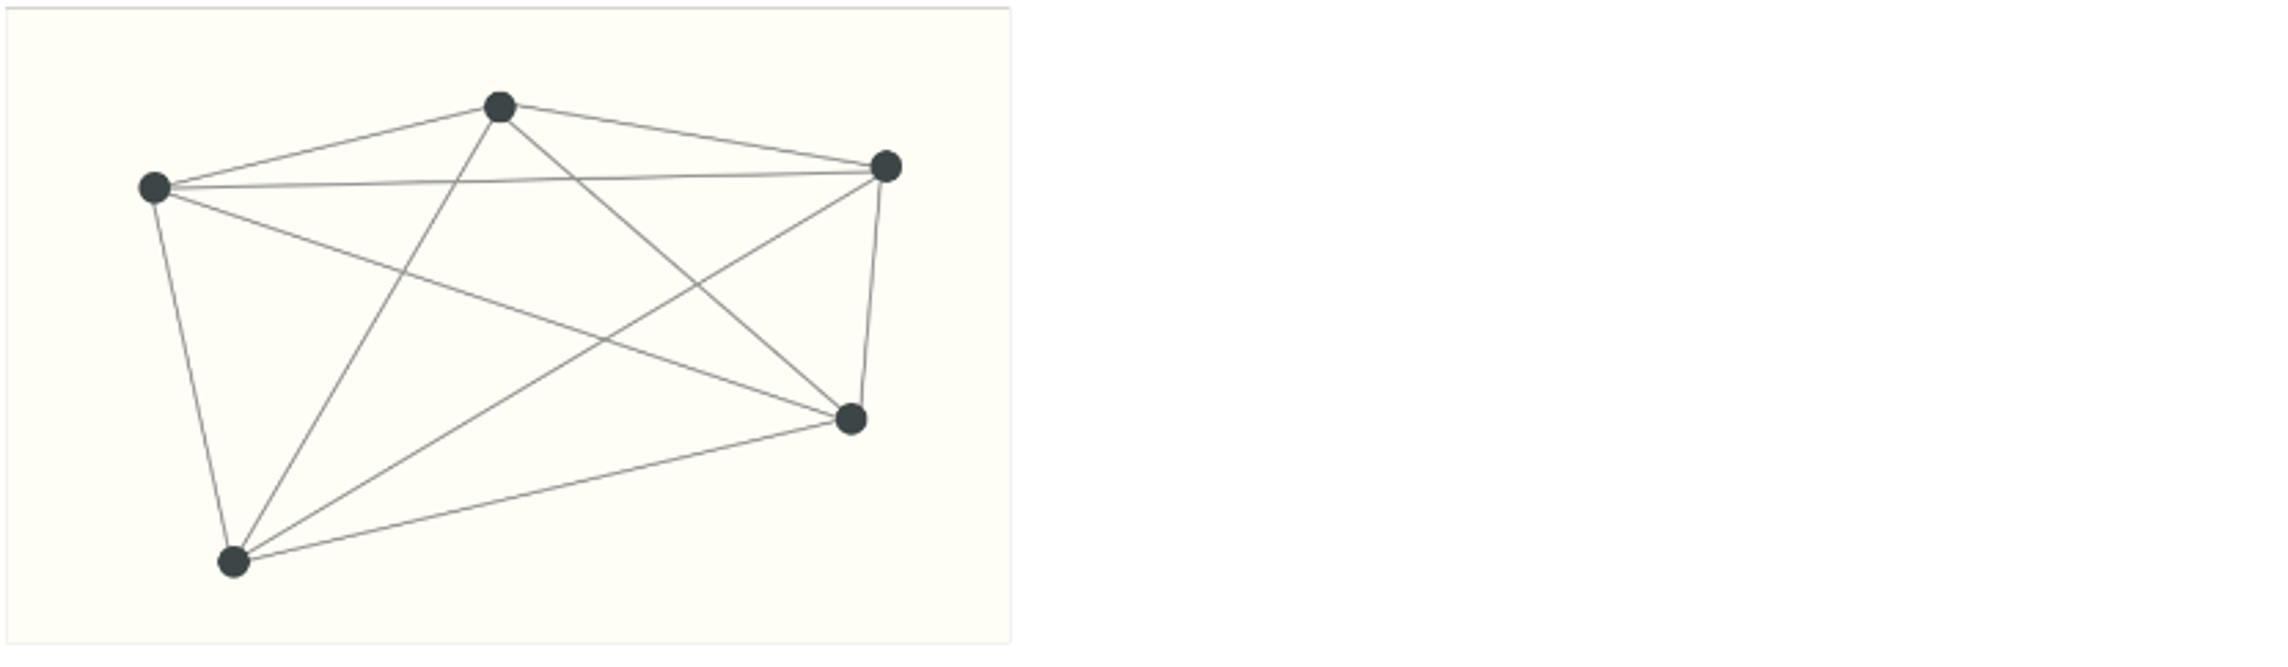
\includegraphics[width=.8\textwidth]{Images/edge-prediction-input.png}
    \end{figure}}

    \only<3>{\begin{figure}
        \centering
        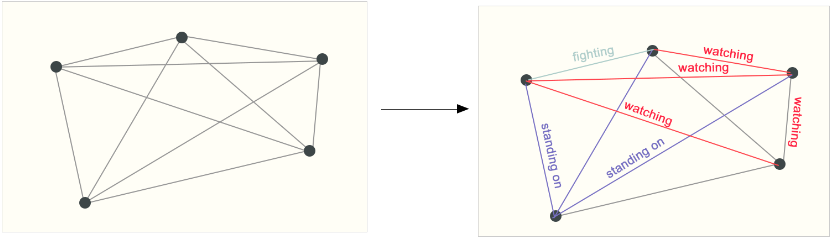
\includegraphics[width=.8\textwidth]{Images/edge-prediction-input-output.png}
    \end{figure}}

    \only<1>{
    \begin{figure}
        \centering
        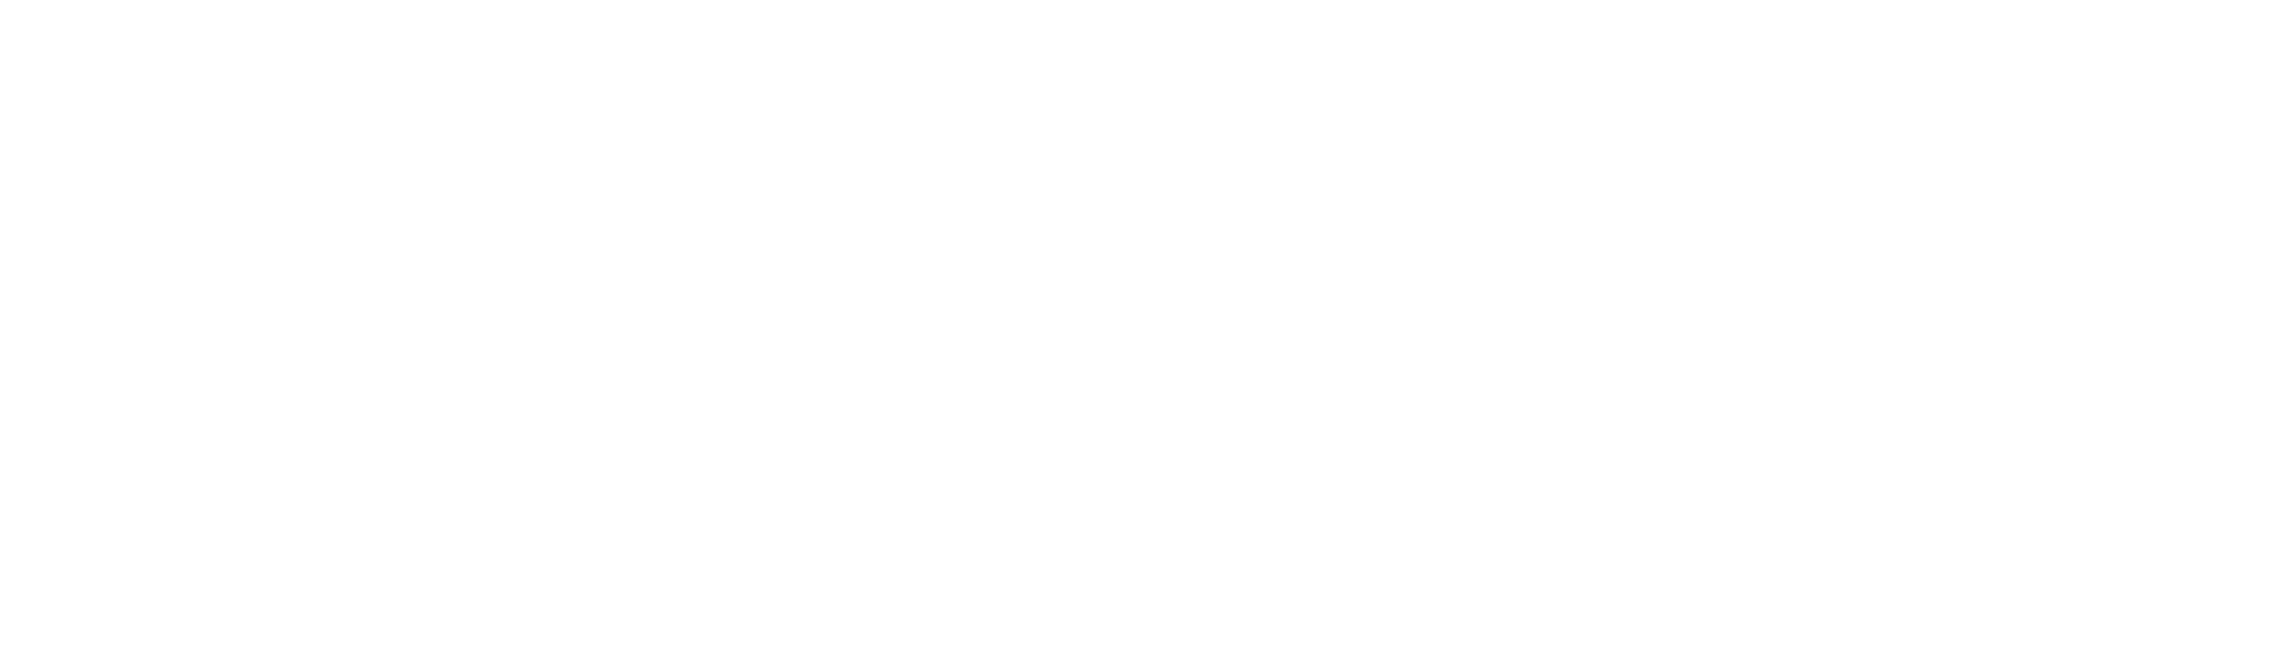
\includegraphics[width=.8\textwidth]{Images/edge-prediction-wh.png}
    \end{figure}
    }}

    \only<5>{
    \begin{figure}
        \centering
        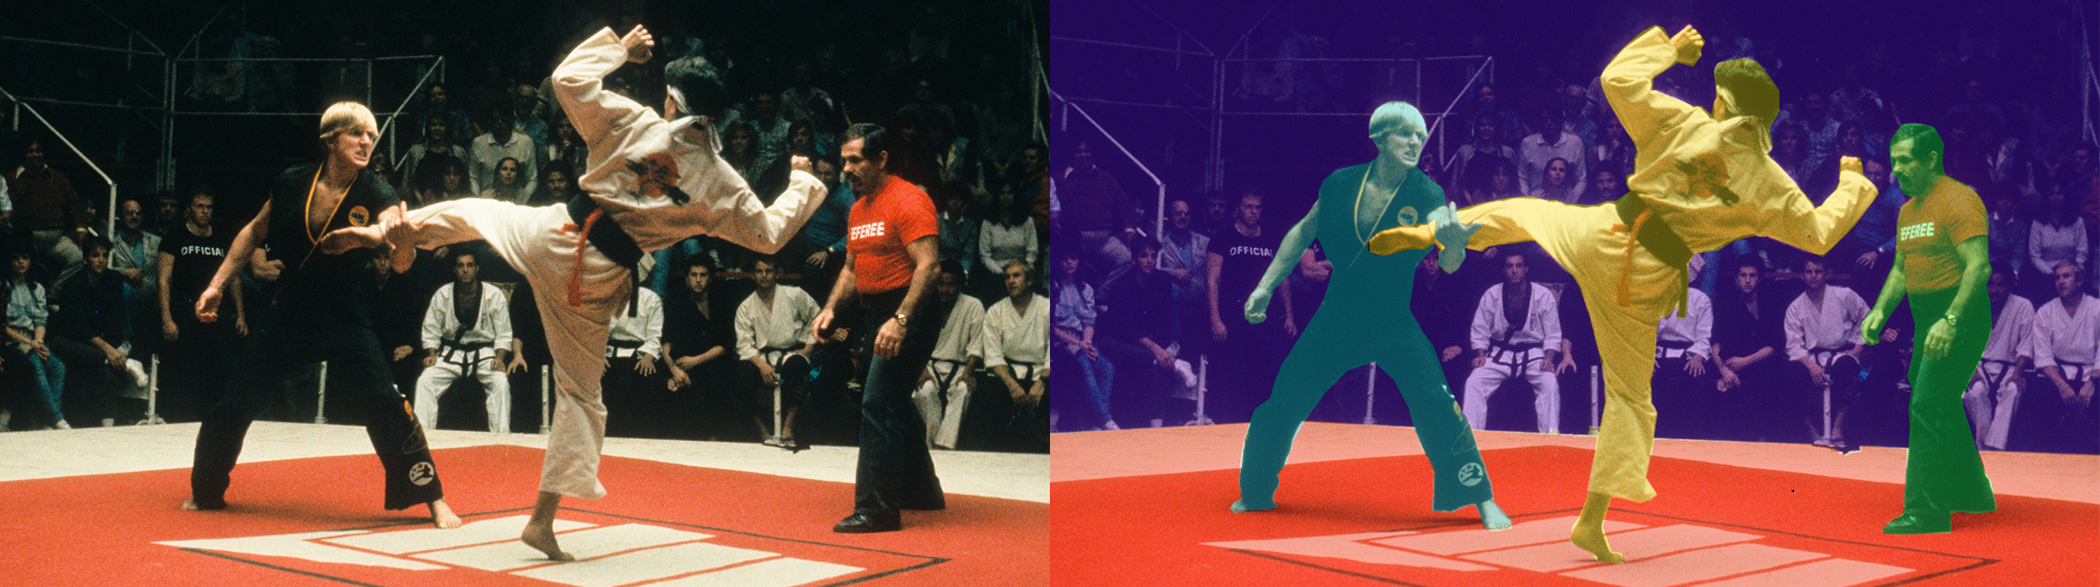
\includegraphics[width=\textwidth]{Images/graph-and-node-level.png}
    \end{figure}
    }

    \only<6>{
    \begin{figure}
        \centering
        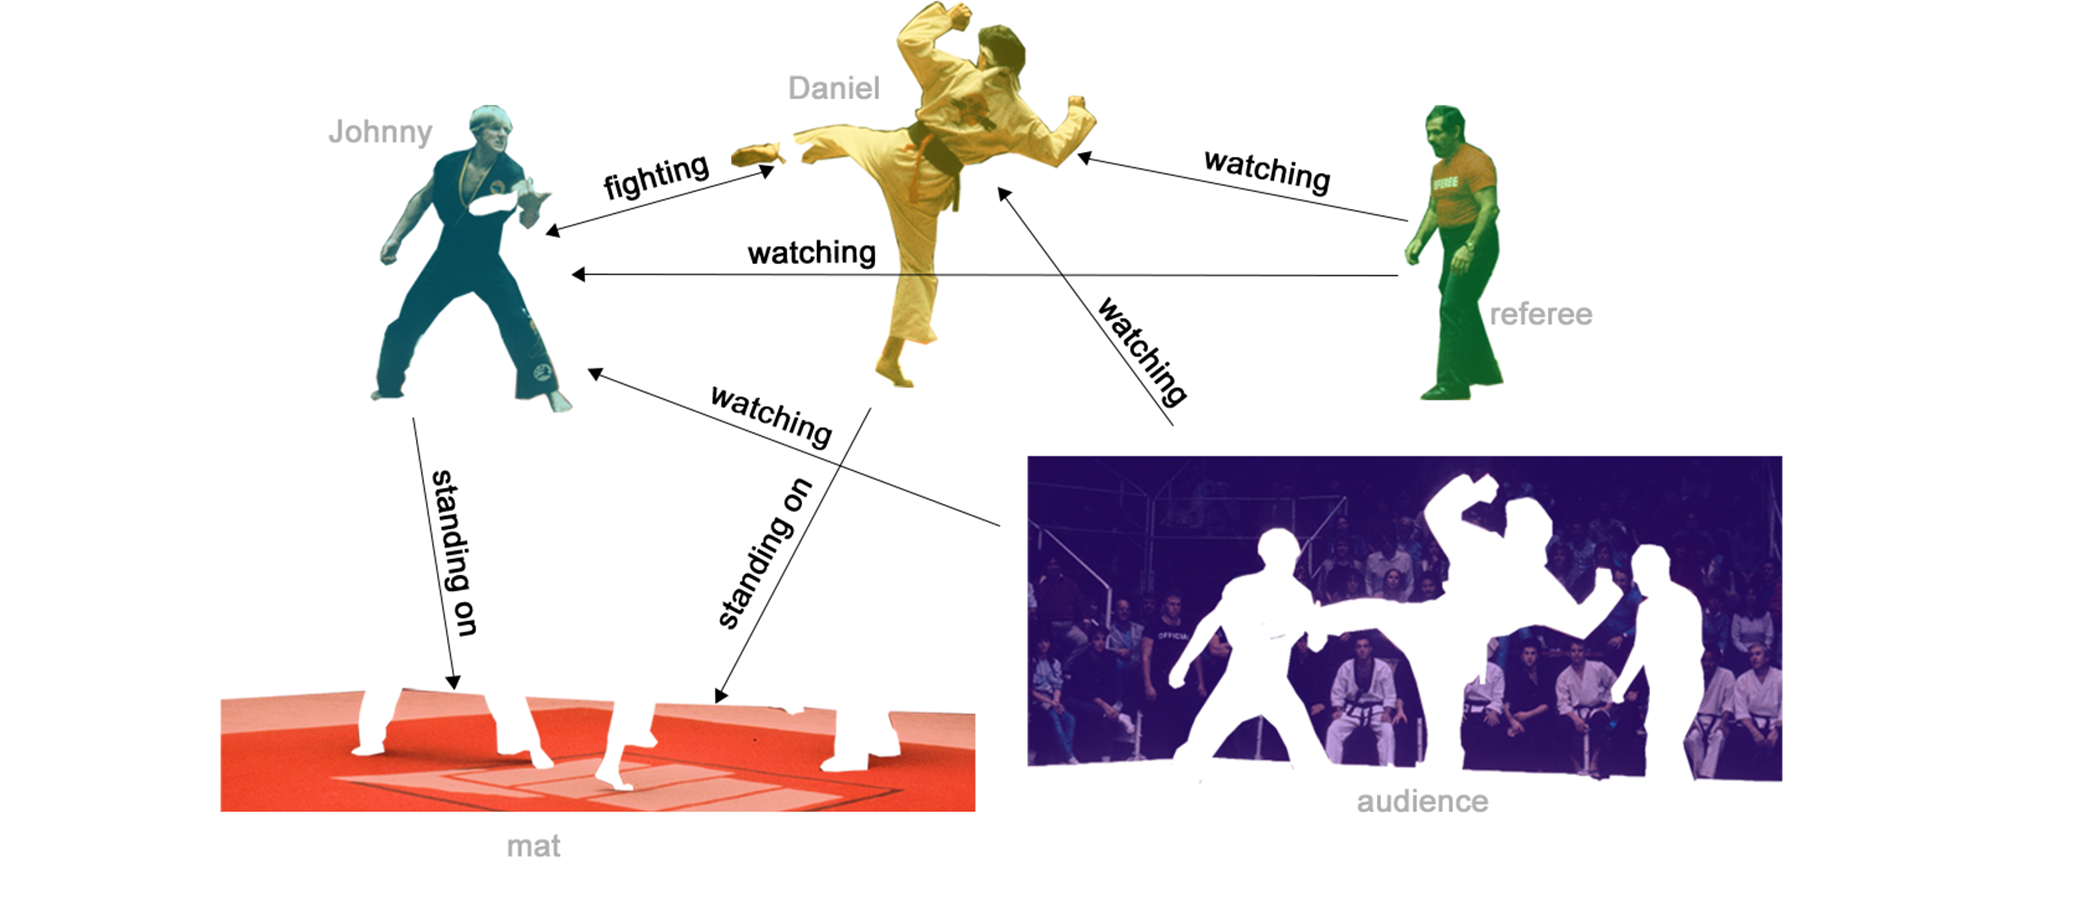
\includegraphics[width=.85\textwidth]{Images/node-and-edge-level.png}
    \end{figure}
    }
\end{frame}

%------------------------------------------------
\subsection{The challenges of using graphs in ML}
\begin{frame}{}
    \centering
    \Large
    How do we go about solving these different graph tasks with neural networks?
\end{frame}

%------------------------------------------------
\begin{frame}{How to Represent Graphs}
    \begin{columns}
        \begin{column}{.5\textwidth}
            \begin{itemize}
                \item[] Graphs have 4 types of information:
                \begin{itemize}
                    \item nodes,
                    \item edges,
                    \item global-context,
                    \item and \only<1>{connectivity}\only<2>{\textbf{connectivity}}!
                \end{itemize}
            \end{itemize}
        \end{column}    

        \only<2>{\vrule}
        
        \begin{column}{.5\textwidth}
            \only<2>{
            \begin{equation*}
                \begin{split}
                    N &= \{ node_i \} \quad [n_{nodes}, node_{dim}] \\
                    E &= \{ edge_i \} \quad [n_{edges}, edge_{dim}] \\ 
                    U &= master \, node's \, embedding \; [, global_{dim}]
                \end{split}
            \end{equation*}}
        \end{column}
    \end{columns}
\end{frame}

%------------------------------------------------
\begin{frame}{Representing Graph's Connectivity}
    \begin{itemize}
        \item One elegant way to represent graphs is as \textbf{Adjacency lists}: These describe the connectivity of edge $e_k$ between nodes $n_i$ and $n_j$ as a tuple $(i,j)$ in the $k$-th entry of an adjacency list.
        \begin{itemize}
            \item memory-efficient (even with sparse matrices),
            \item permutation invariant.
        \end{itemize}
    \end{itemize}
\end{frame}

%------------------------------------------------
%\begin{frame}{Representing Graph's Connectivity}
%    \begin{figure}
%        \centering
%        \includegraphics{Images/adjacency-list.png}
%    \end{figure}
%\end{frame}

%------------------------------------------------
\section{Graph Neural Networks}
%------------------------------------------------
\subsection{The simplest GNN}
\begin{frame}{}
    \begin{itemize}
        \item \textbf{GNN}s = \textbf{G}raph \textbf{N}eural \textbf{N}etworks
        \item \textbf{A GNN is an optimizable transformation on all attributes of the graph }(i.e., nodes, edges, global-context) \textbf{that preserves graph symmetries} (connectivity or permutation invariances)
        \item \textit{"graph-in, graph-out"} architecture
    \end{itemize}
\end{frame}

%------------------------------------------------
\begin{frame}{The Simplest GNN}
    \begin{figure}
        \centering
        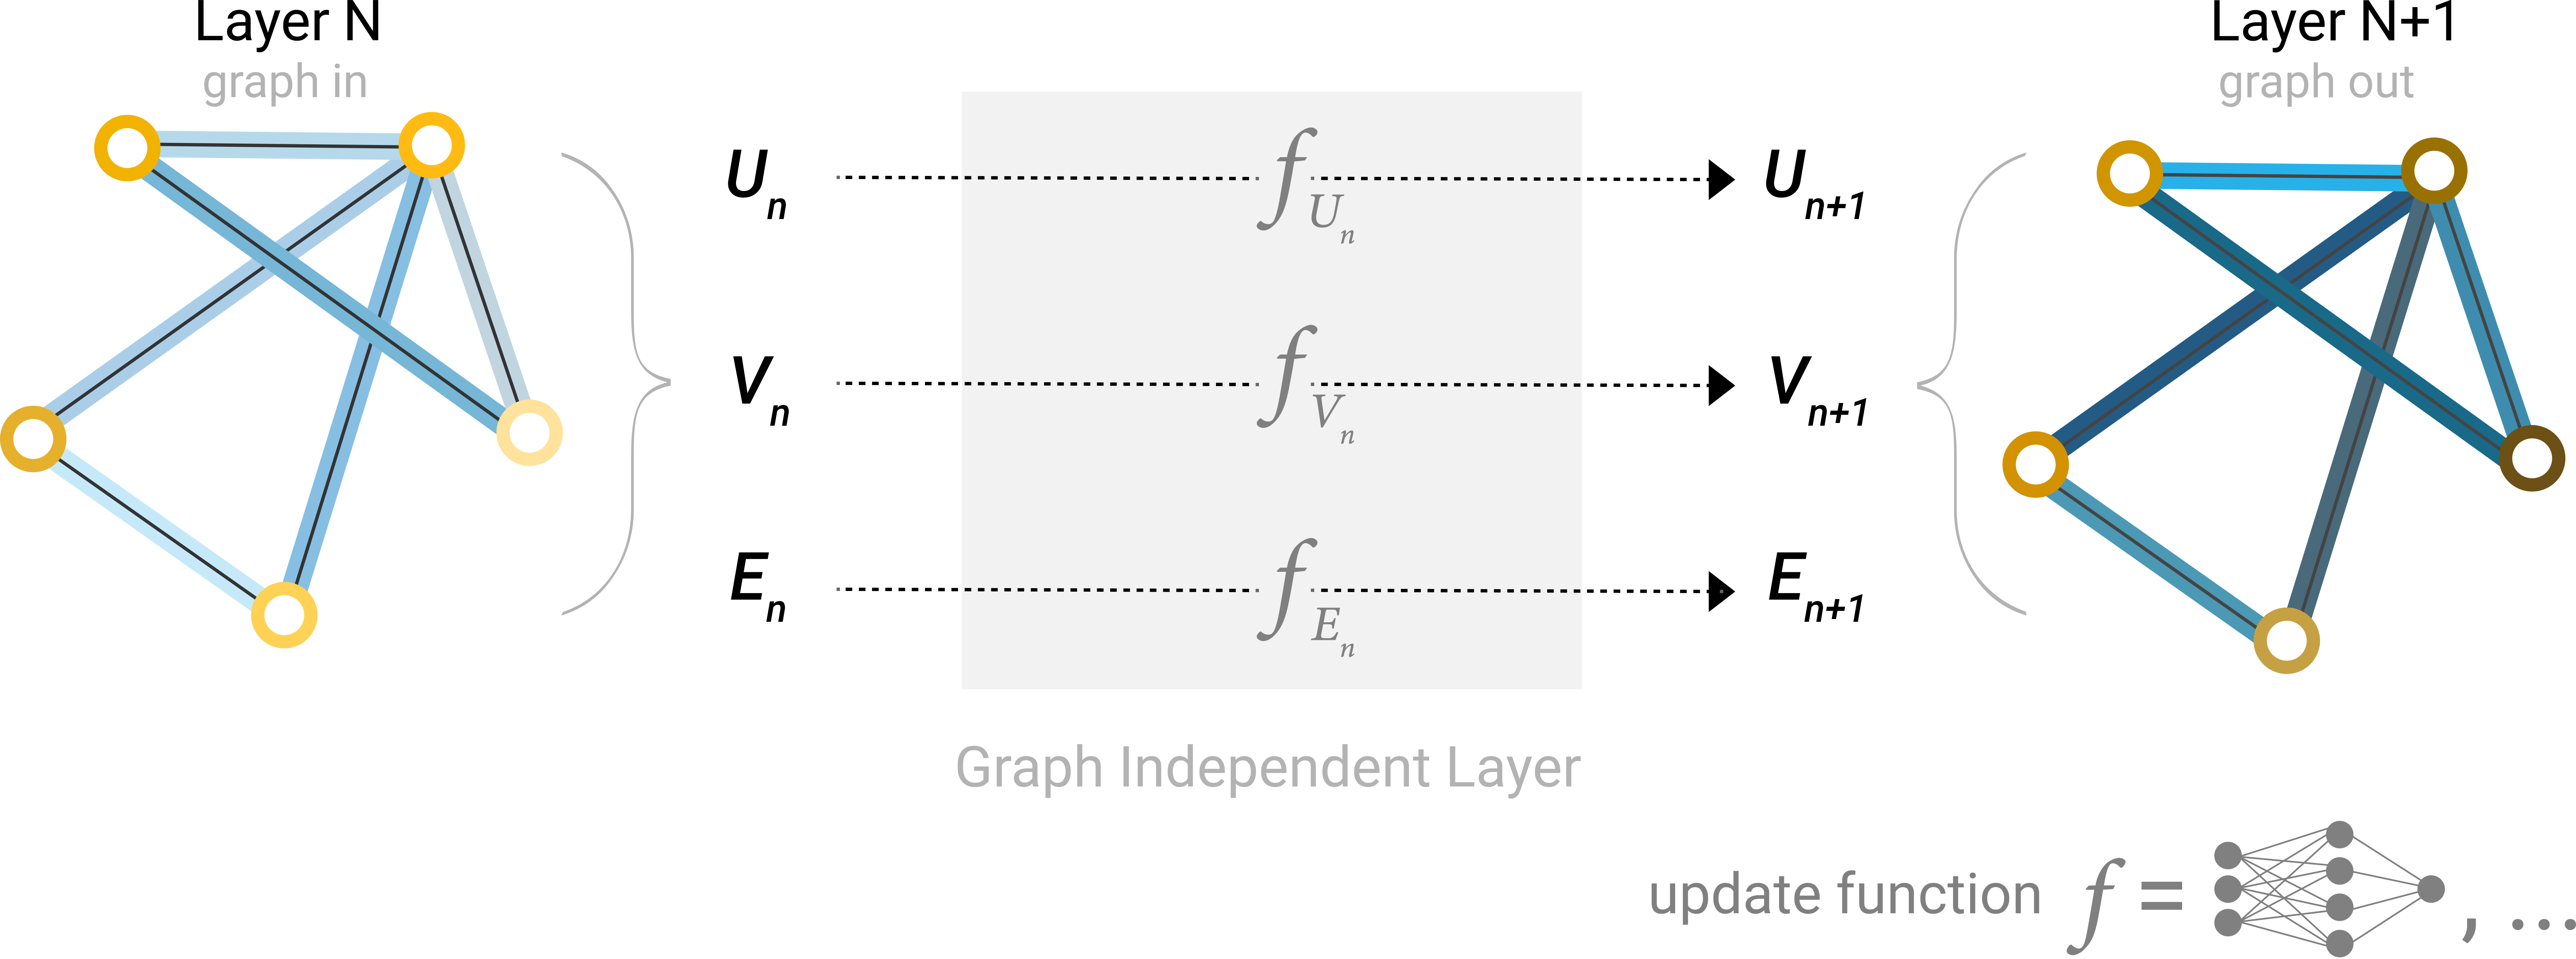
\includegraphics[width=.9\textwidth]{Images/simplest-gnn.png}
    \end{figure}
\end{frame}

%------------------------------------------------
\subsection{GNN Predictions by Pooling Information}
%------------------------------------------------
\begin{frame}{GNN Predictions}
    \begin{figure}
        \centering
        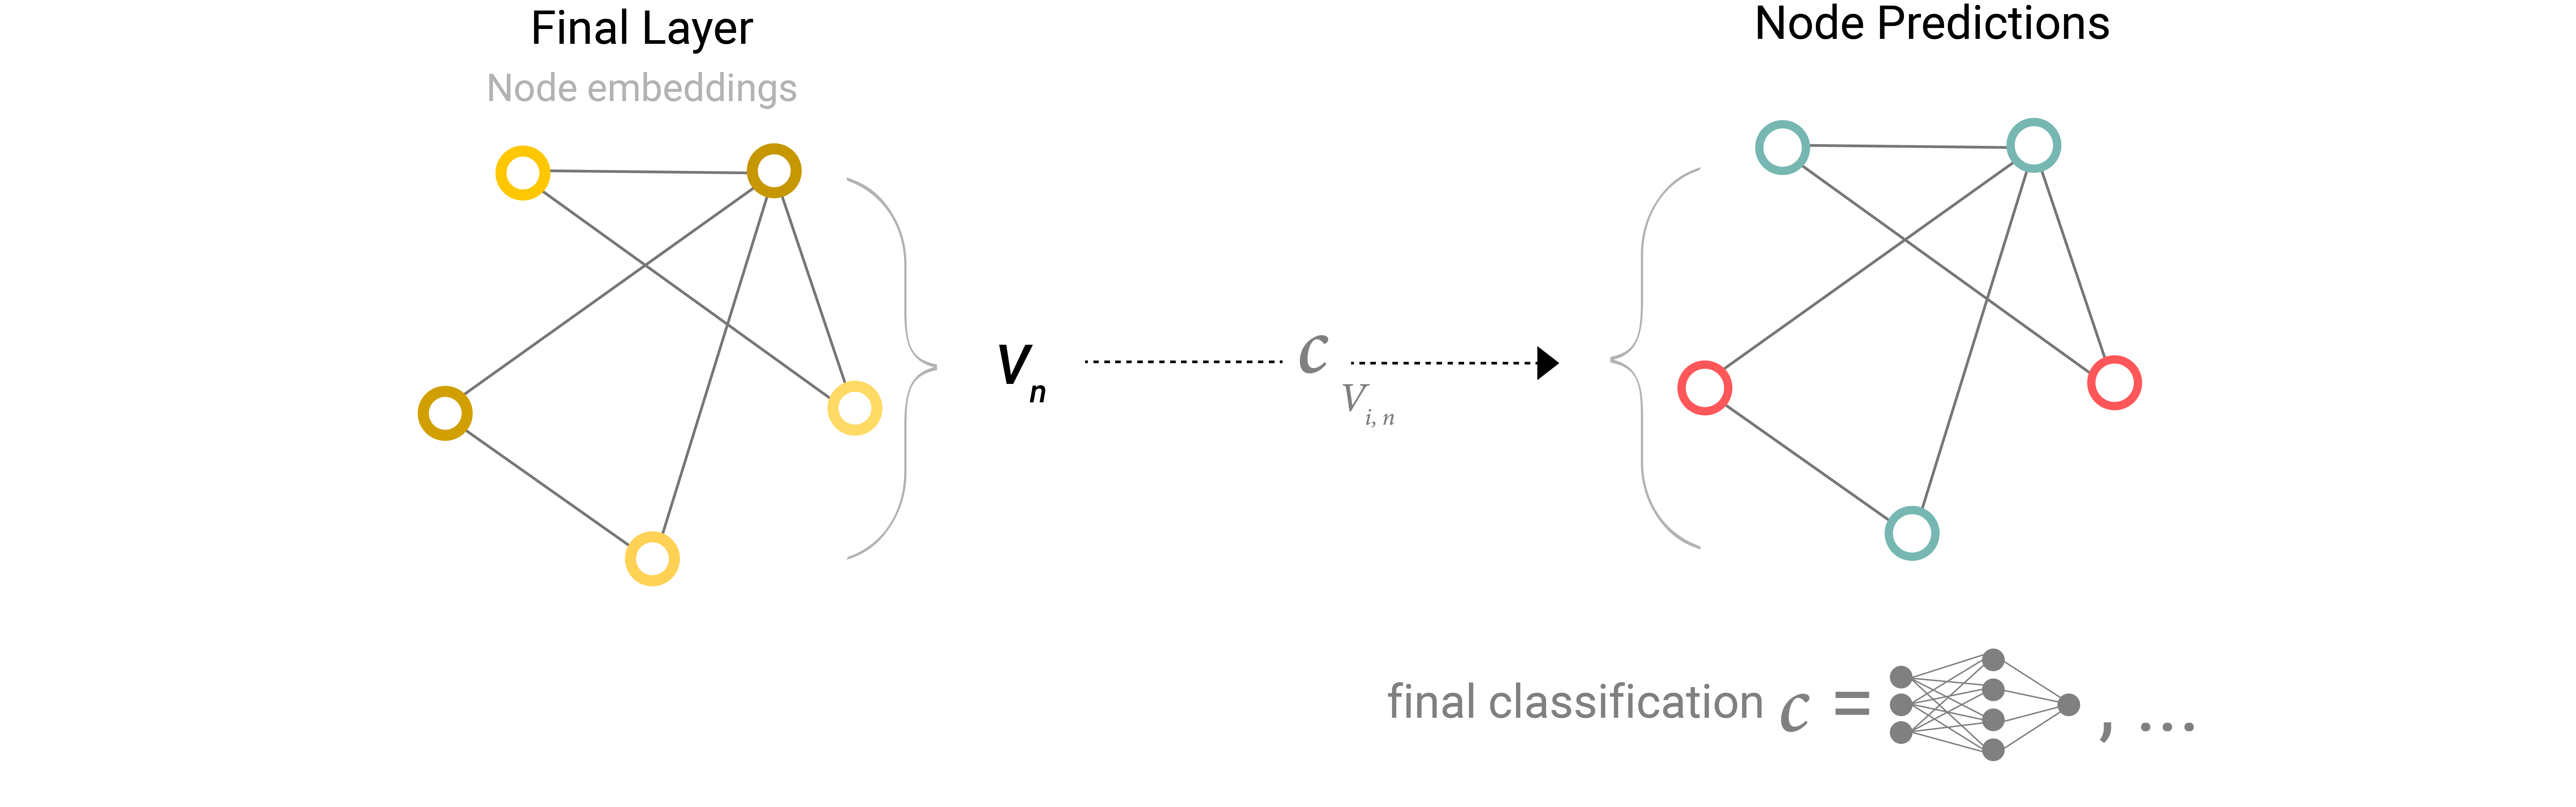
\includegraphics[width=\textwidth]{Images/gnn-prediction.png}
    \end{figure}
\end{frame}

%------------------------------------------------
\begin{frame}{Pooling Information}
    \justifying
    \begin{itemize}[<+->]
        \item \textbf{Pooling}: Collecting information from 1 component and giving them to another.
        \vspace{.5em}
        \begin{enumerate}
            \itemsep.5em
            \item For each item to be pooled, \textit{gather} each of their embeddings and concatenate them into a matrix.
            \item The gathered embeddings are then \textit{aggregated}, using via a operation (e.g., sum, mean).
        \end{enumerate}

        \item Abbreviation: $\mathbf{\rho}$ e.g., gathering information from edges to nodes $\rho_{E_n \rightarrow V_n}$.
    \end{itemize}
\end{frame}

%------------------------------------------------
\begin{frame}{Pooling Information}
    \only<1>{
    \begin{figure}
        \centering
        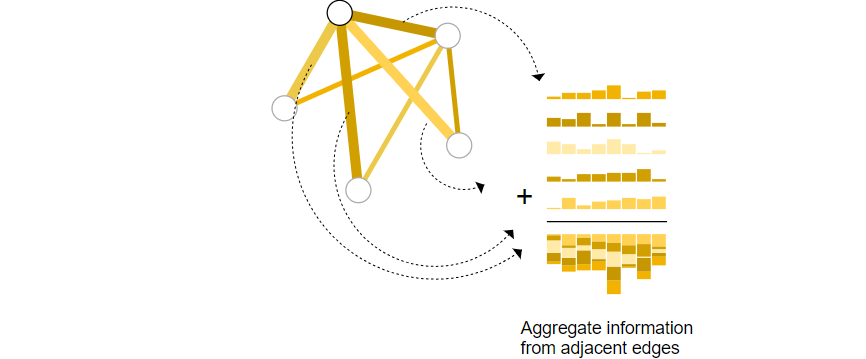
\includegraphics[width=.75\textwidth]{Images/pooling-edges-1.png}
    \end{figure}
    }

    \only<2>{
    \begin{figure}
        \centering
        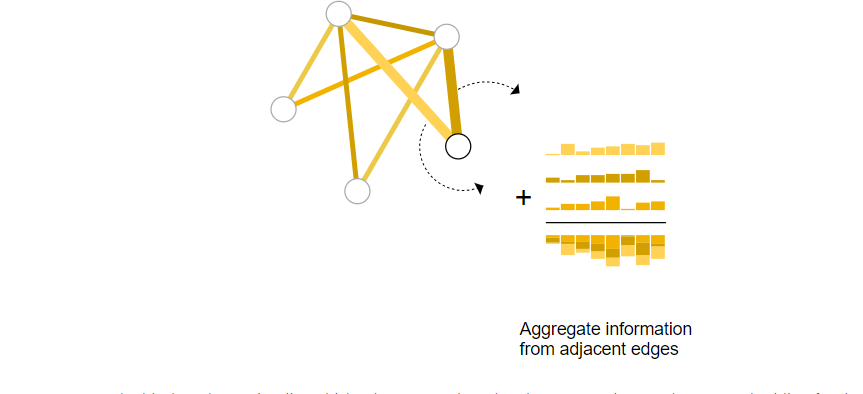
\includegraphics[width=.75\textwidth]{Images/pooling-edges-2.png}
    \end{figure}
    }
\end{frame}

%------------------------------------------------
\begin{frame}{GNN Predictions by Pooling Information}
    \only<1>{
    \begin{figure}
        \centering
        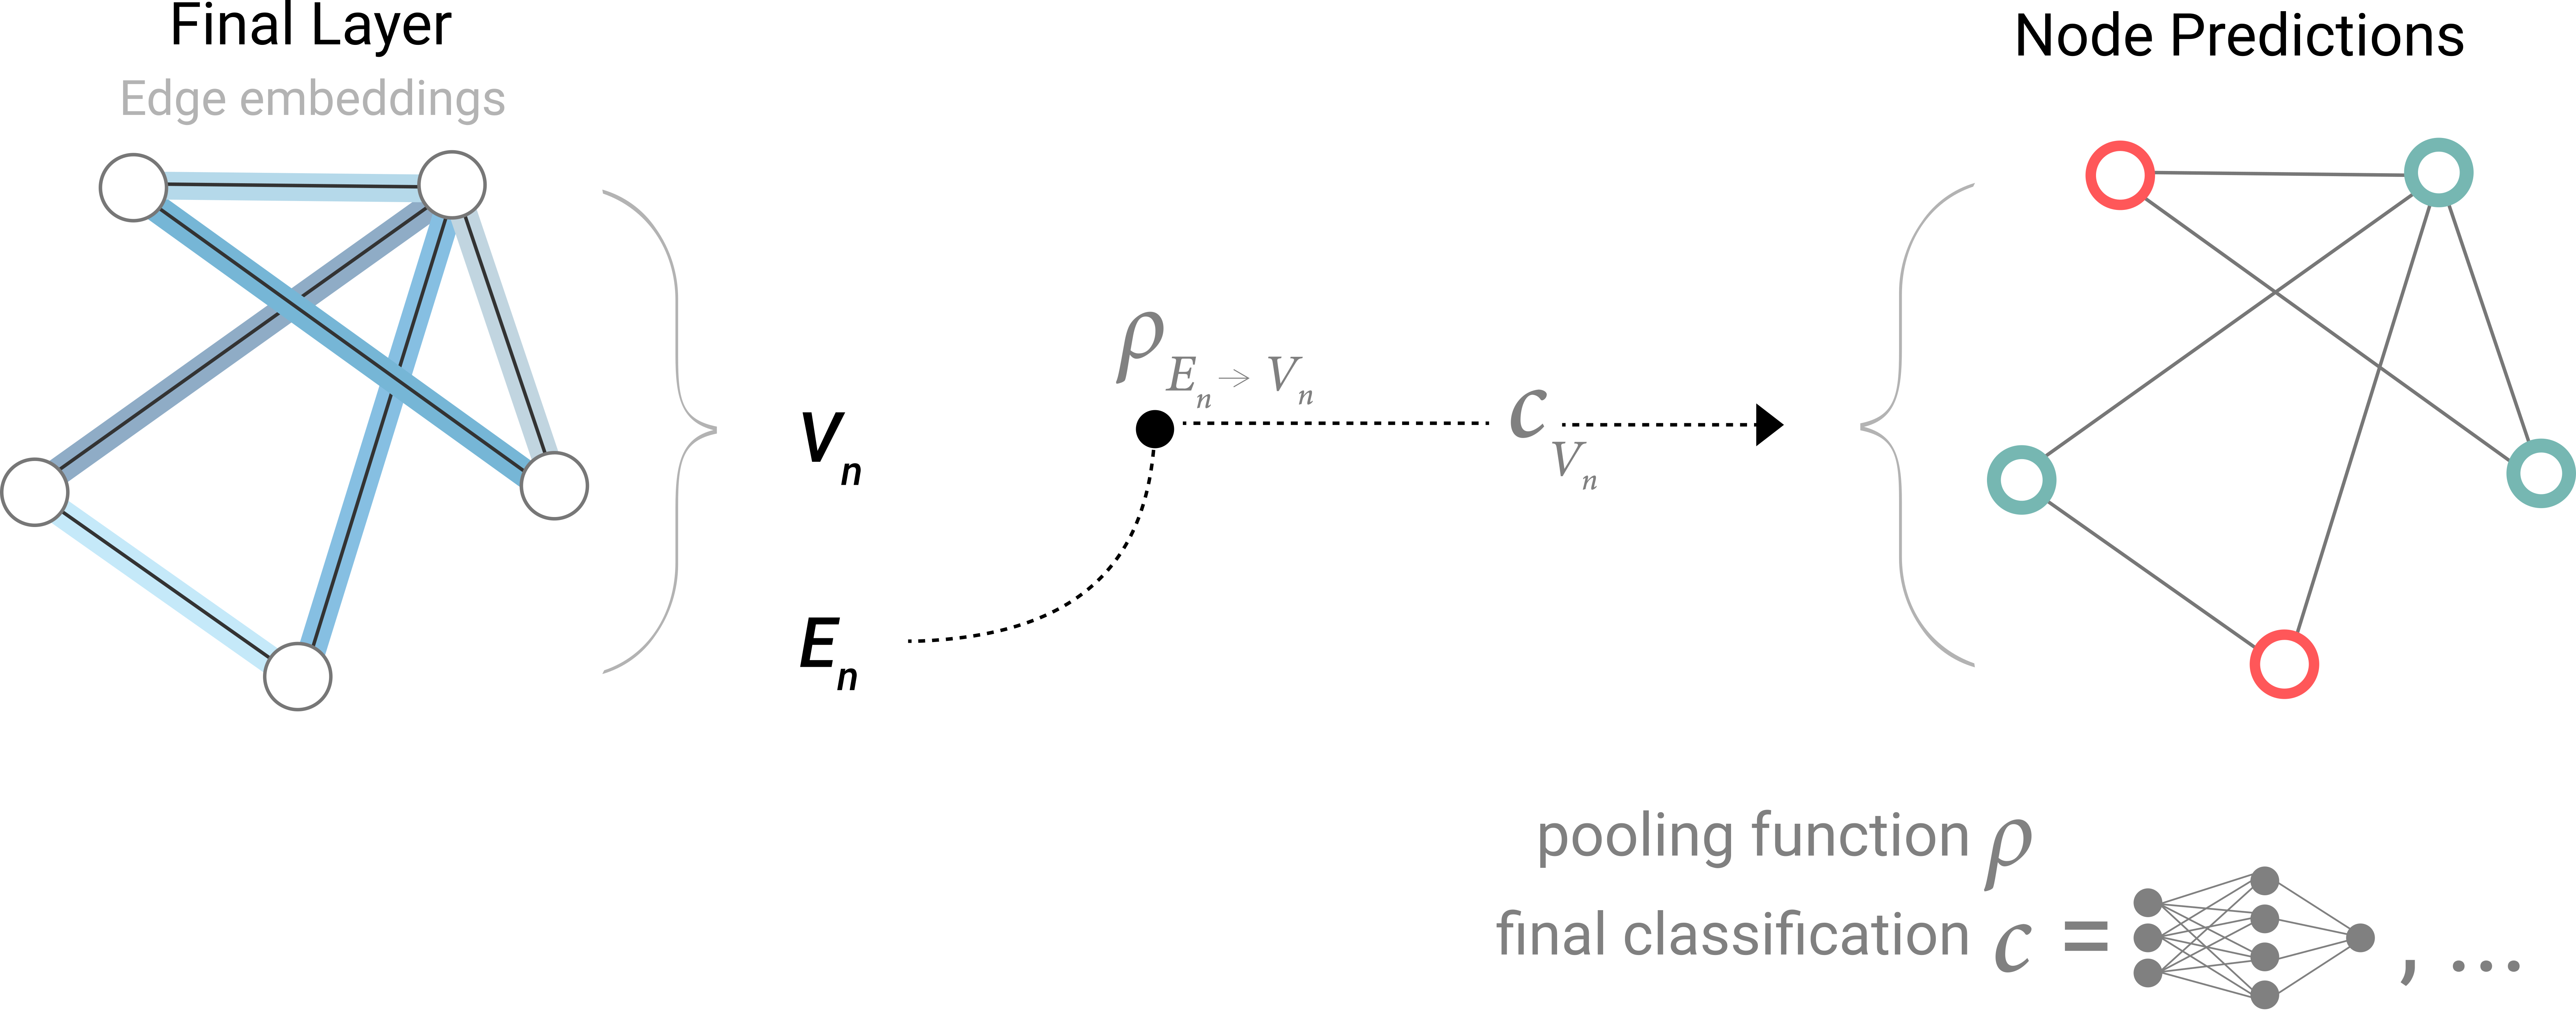
\includegraphics[width=.75\textwidth]{Images/nodes-prediction-pooling-edges.png}
    \end{figure}
    }

    \only<2>{
    \begin{figure}
        \centering
        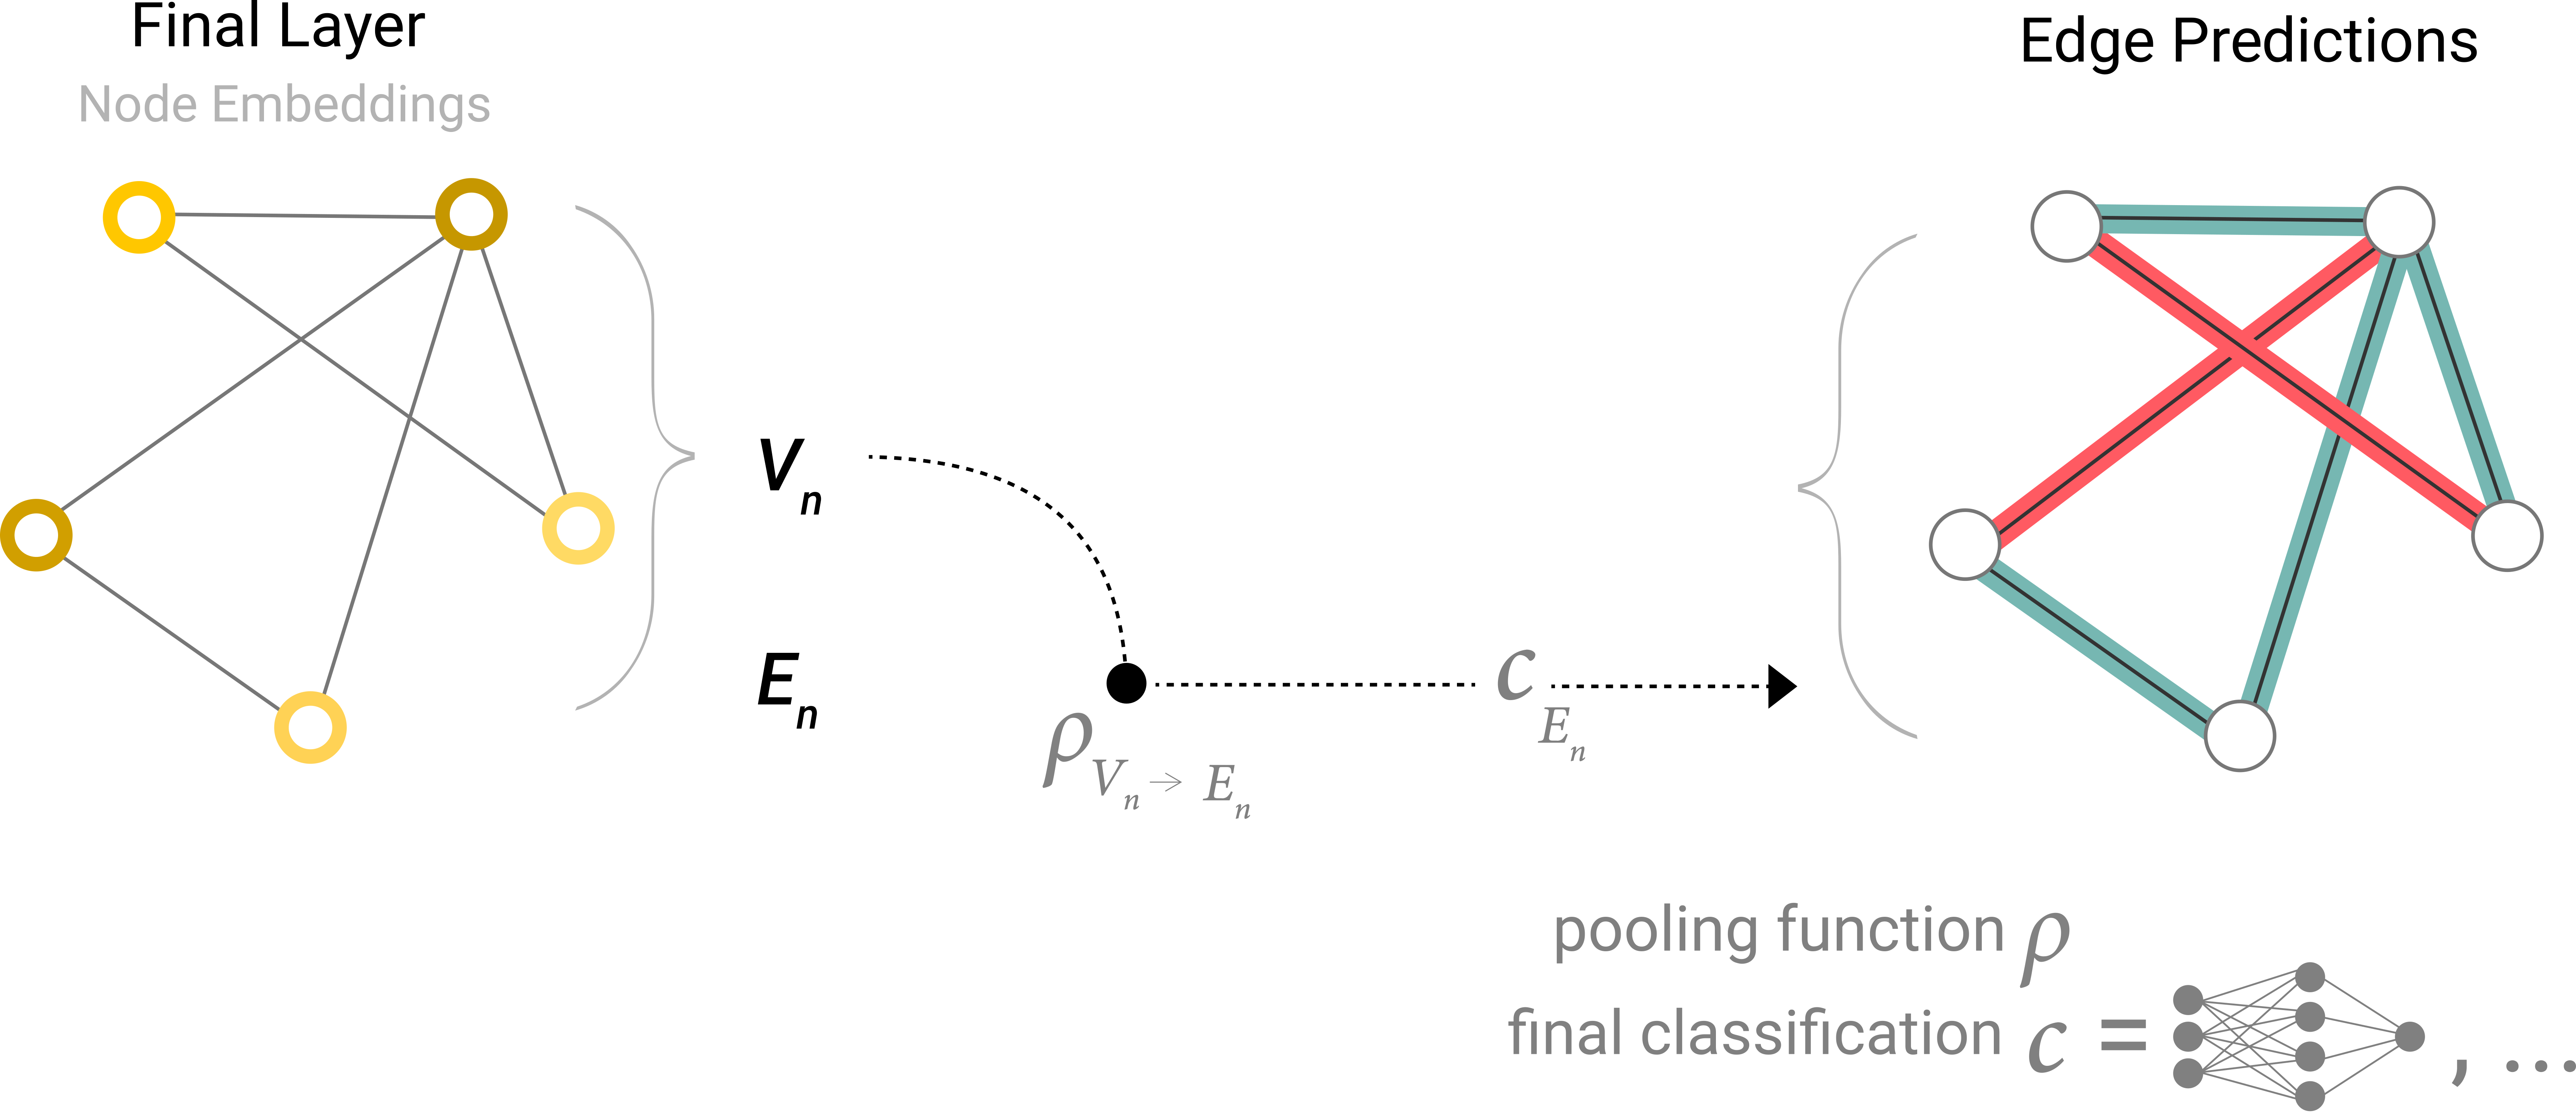
\includegraphics[width=.75\textwidth]{Images/edges-prediction-pooling-nodes.png}
    \end{figure}
    }

    \only<3>{
    \begin{figure}
        \centering
        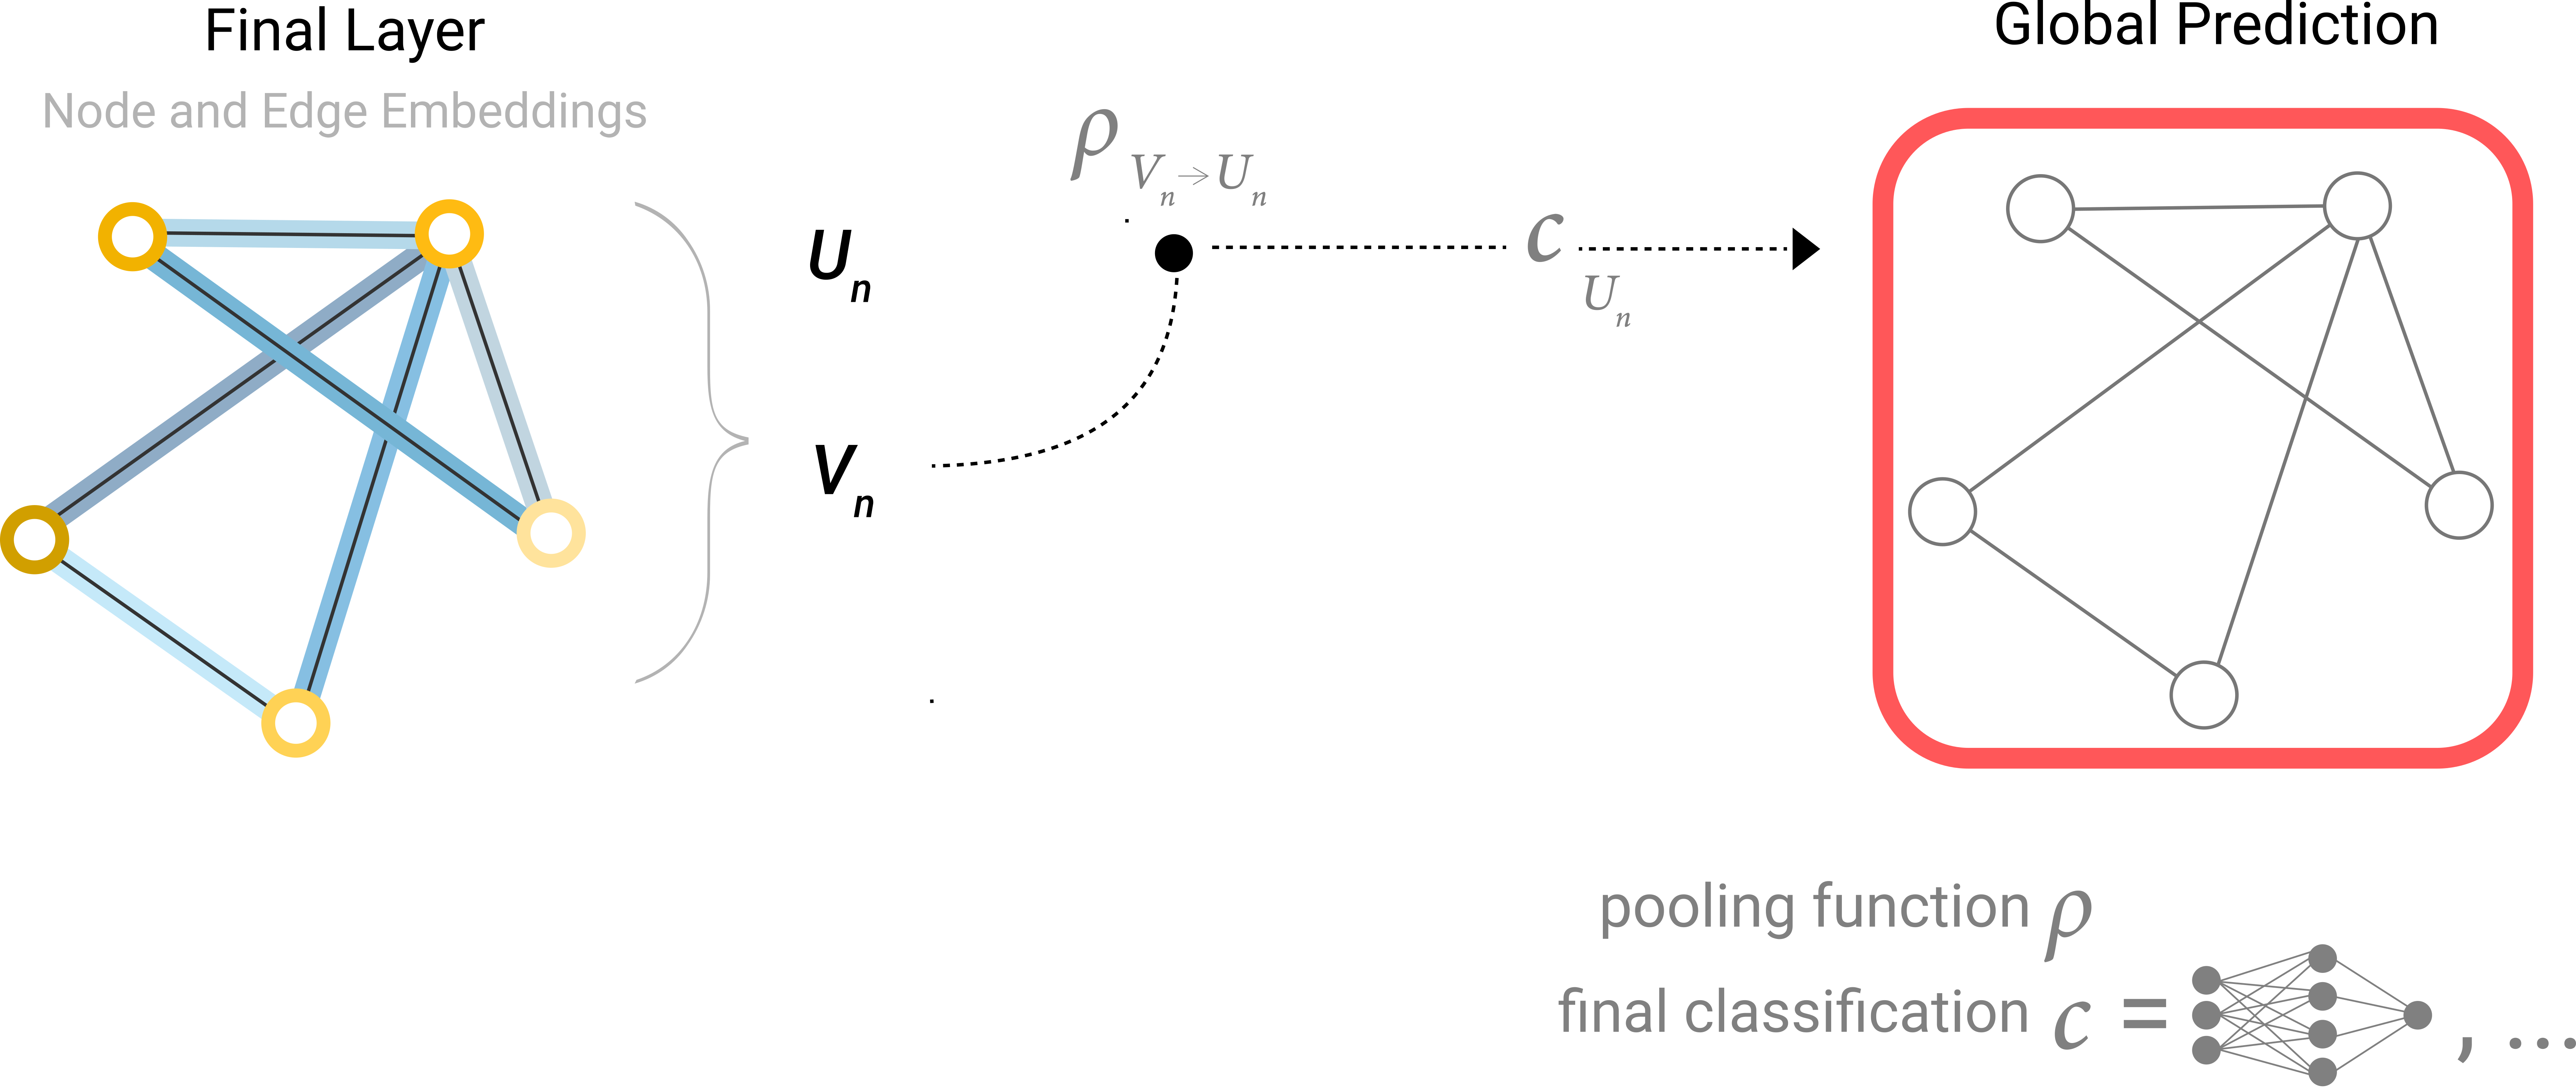
\includegraphics[width=.75\textwidth]{Images/graph-prediction-pooling-nodes.png}
    \end{figure}
    }
\end{frame}

%------------------------------------------------
\begin{frame}{End2End Prediction Task with a GNN Model}
    \begin{figure}
        \centering
        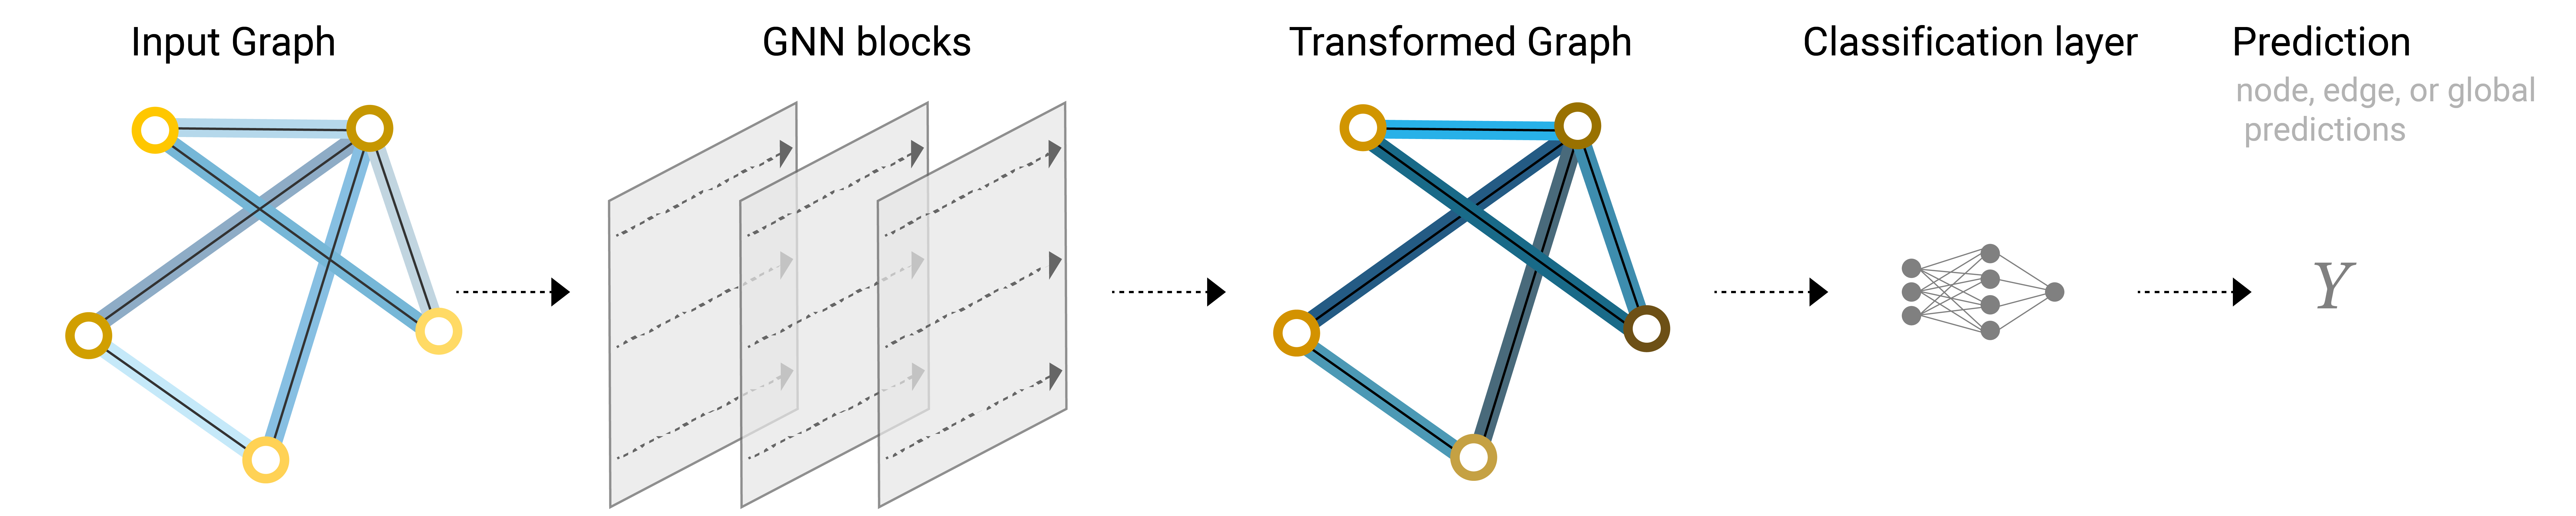
\includegraphics[width=.75\textwidth]{Images/end2end-prediction.png}
    \end{figure}
\end{frame}

%------------------------------------------------
\begin{frame}{End2End Prediction Task with a GNN Model}
    \begin{itemize}
        \item We still don't use the connectivity of the graph
        \begin{itemize}
            \item Each component is processed independently
            \item ONLY use connectivity when prediction
        \end{itemize}
    \end{itemize}
\end{frame}

%------------------------------------------------
\subsection{Passing messages between parts of the graph}
%------------------------------------------------
\begin{frame}{}
    \centering
    ...What if we try using pooling inside GNN Layers?
    \vspace{1cm}
    
    \only<2>{
    Or to make our learned embeddings aware of graph \textbf{connectivity}?
    }
\end{frame}

%------------------------------------------------
\begin{frame}{Message Passing}
    \begin{itemize}
        \item \textbf{Message Passing:}
        \vspace{.5em}
        \begin{enumerate}
            \itemsep.5em
            \item For each node in the graph, \textit{gather} all the neighboring node embedding (or messages), which is the $g$ function described above.
            \item \textit{Aggregate} all messages via an aggregate function (e.g, sum).
            \item All pooled messages are passed through an \textit{update function}, ussually a learned neural network.
        \end{enumerate}

        \item Just as pooling can be applied to either nodes or edges, message passing can occur between either nodes or edges.
    \end{itemize}
\end{frame}

%------------------------------------------------
\begin{frame}{Message Passing}
    \begin{figure}
        \centering
        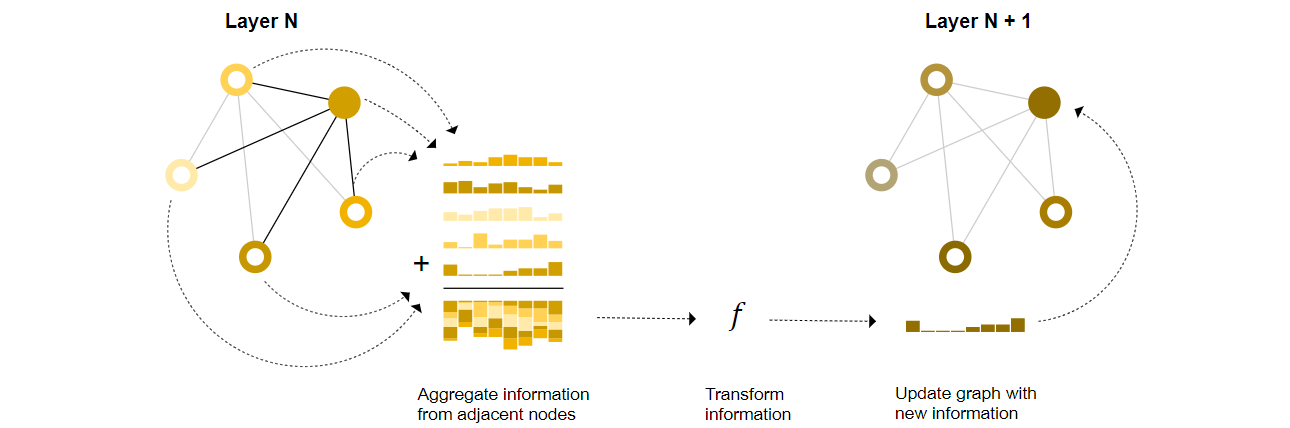
\includegraphics[width=.8\textwidth]{Images/message-passing.png}
    \end{figure}
\end{frame}

%------------------------------------------------
\begin{frame}{GCN architecture}
    \begin{figure}
        \centering
        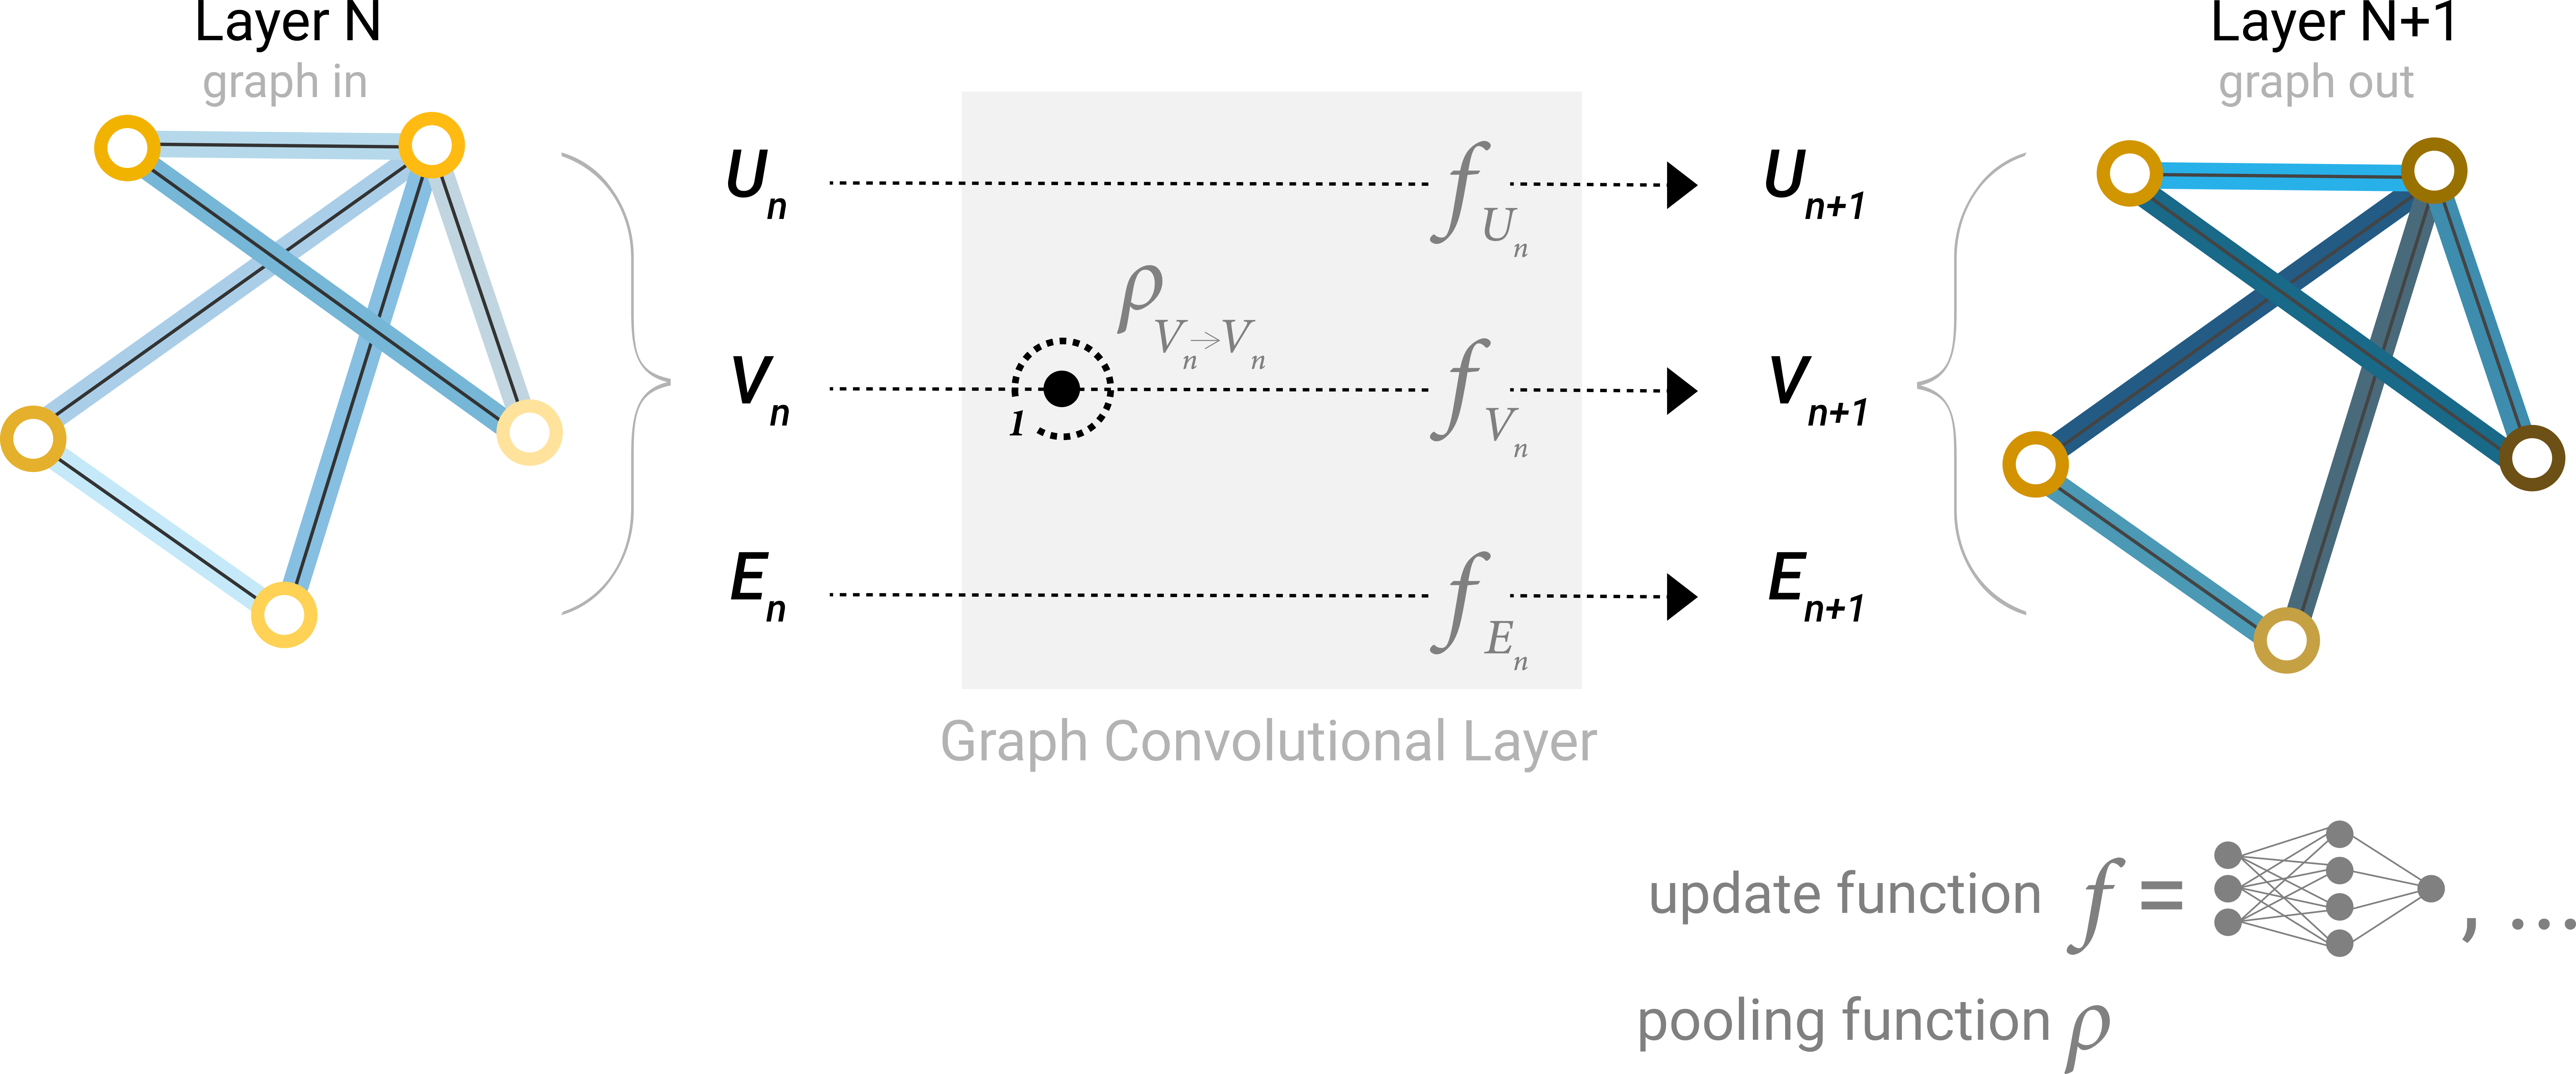
\includegraphics[width=.8\textwidth]{Images/GCN-schematic.png}
    \end{figure}
\end{frame}

%------------------------------------------------
\begin{frame}{Learning Edge Representations}
    \begin{figure}
        \centering
        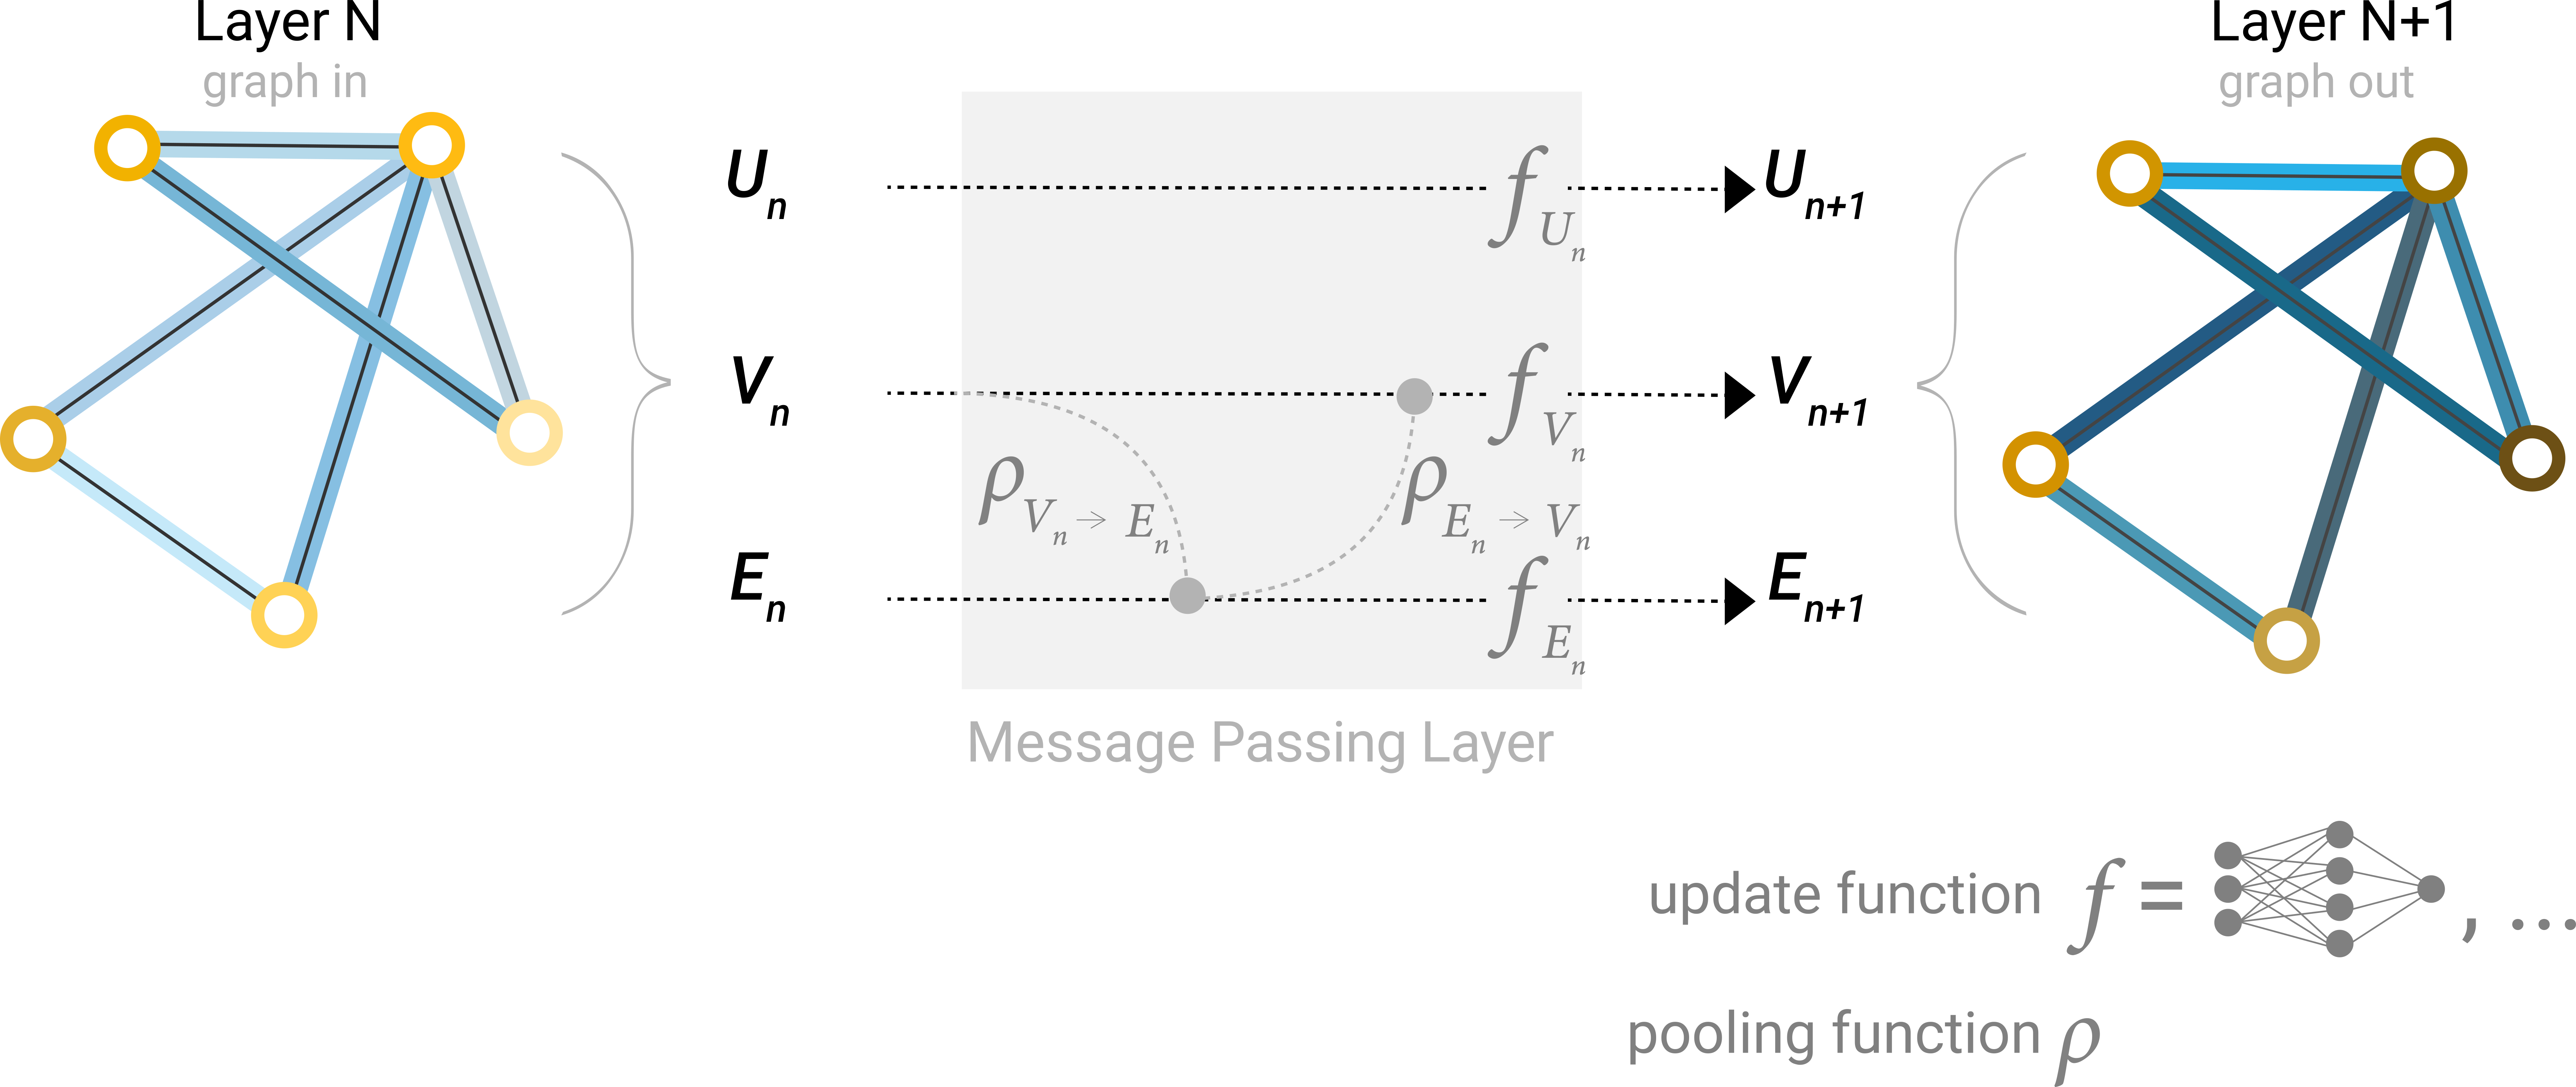
\includegraphics[width=.8\textwidth]{Images/message-passing-schematic.png}
    \end{figure}
\end{frame}

%------------------------------------------------
\begin{frame}{Adding Global Representations}
    \begin{itemize}
        \item So far, there is still one flaw:
        \begin{itemize}
            \itemsep.5em
            \item Nodes that far away from each other in the graph may never be able to efficiently transfer information to one another, even which several layers.
            \item e.g., if we have $k$-layers, information will propagate at most $k$-steps away.
        \end{itemize}

        \item One solution is by using the global representations or \textbf{master node}.
    \end{itemize}
\end{frame}

%------------------------------------------------
\begin{frame}{Adding Global Representations}
    \only<1>{
    \begin{figure}
        \centering
        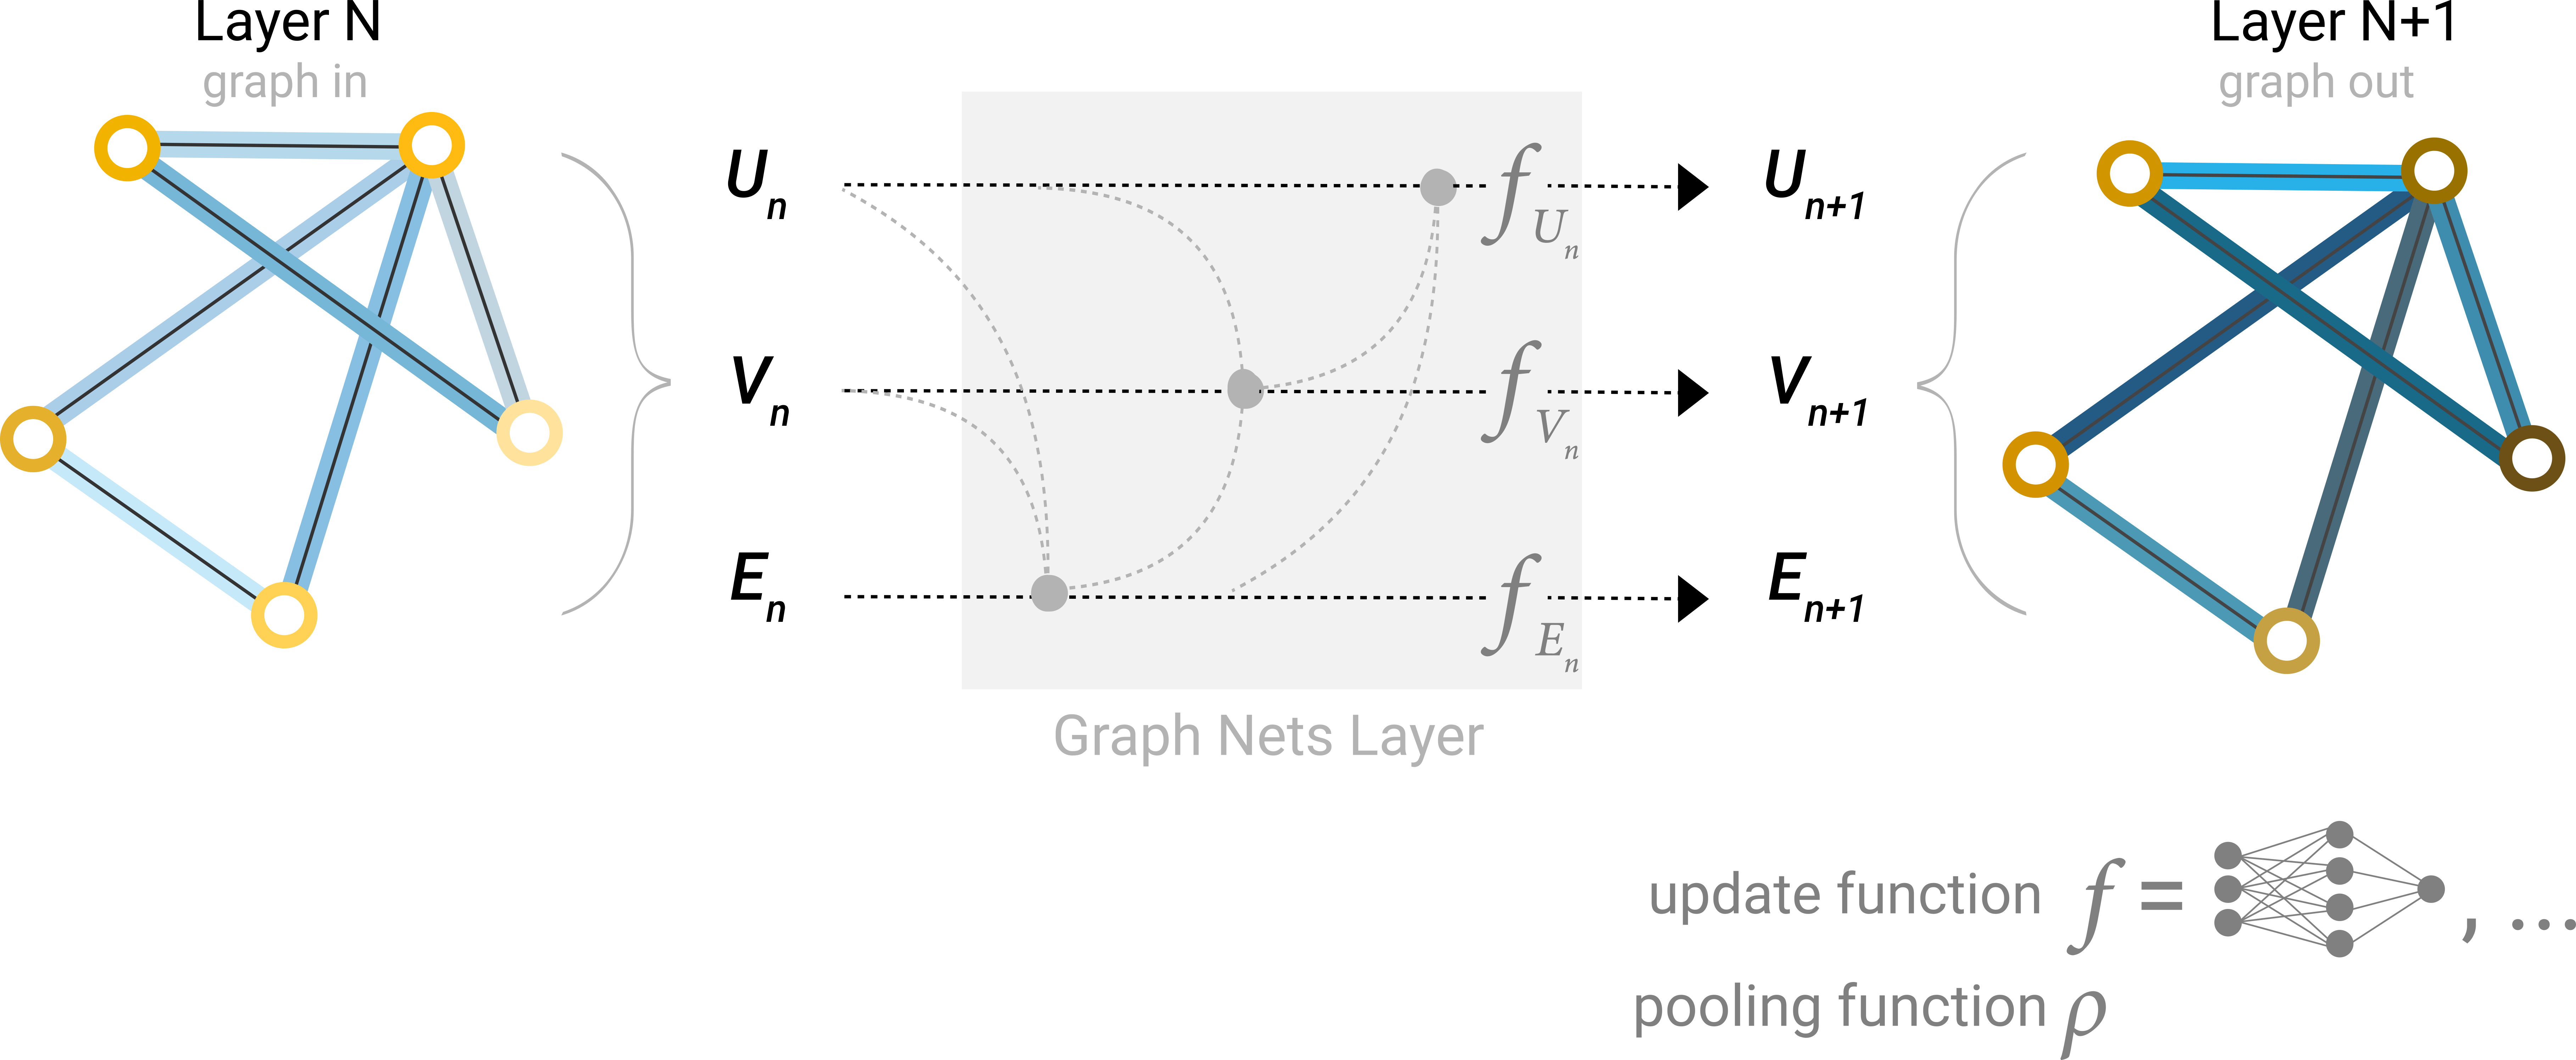
\includegraphics[width=.8\textwidth]{Images/graph-net-schematic-with-global-representations.png}
    \end{figure}}

    \only<2>{
    \begin{figure}
        \centering
        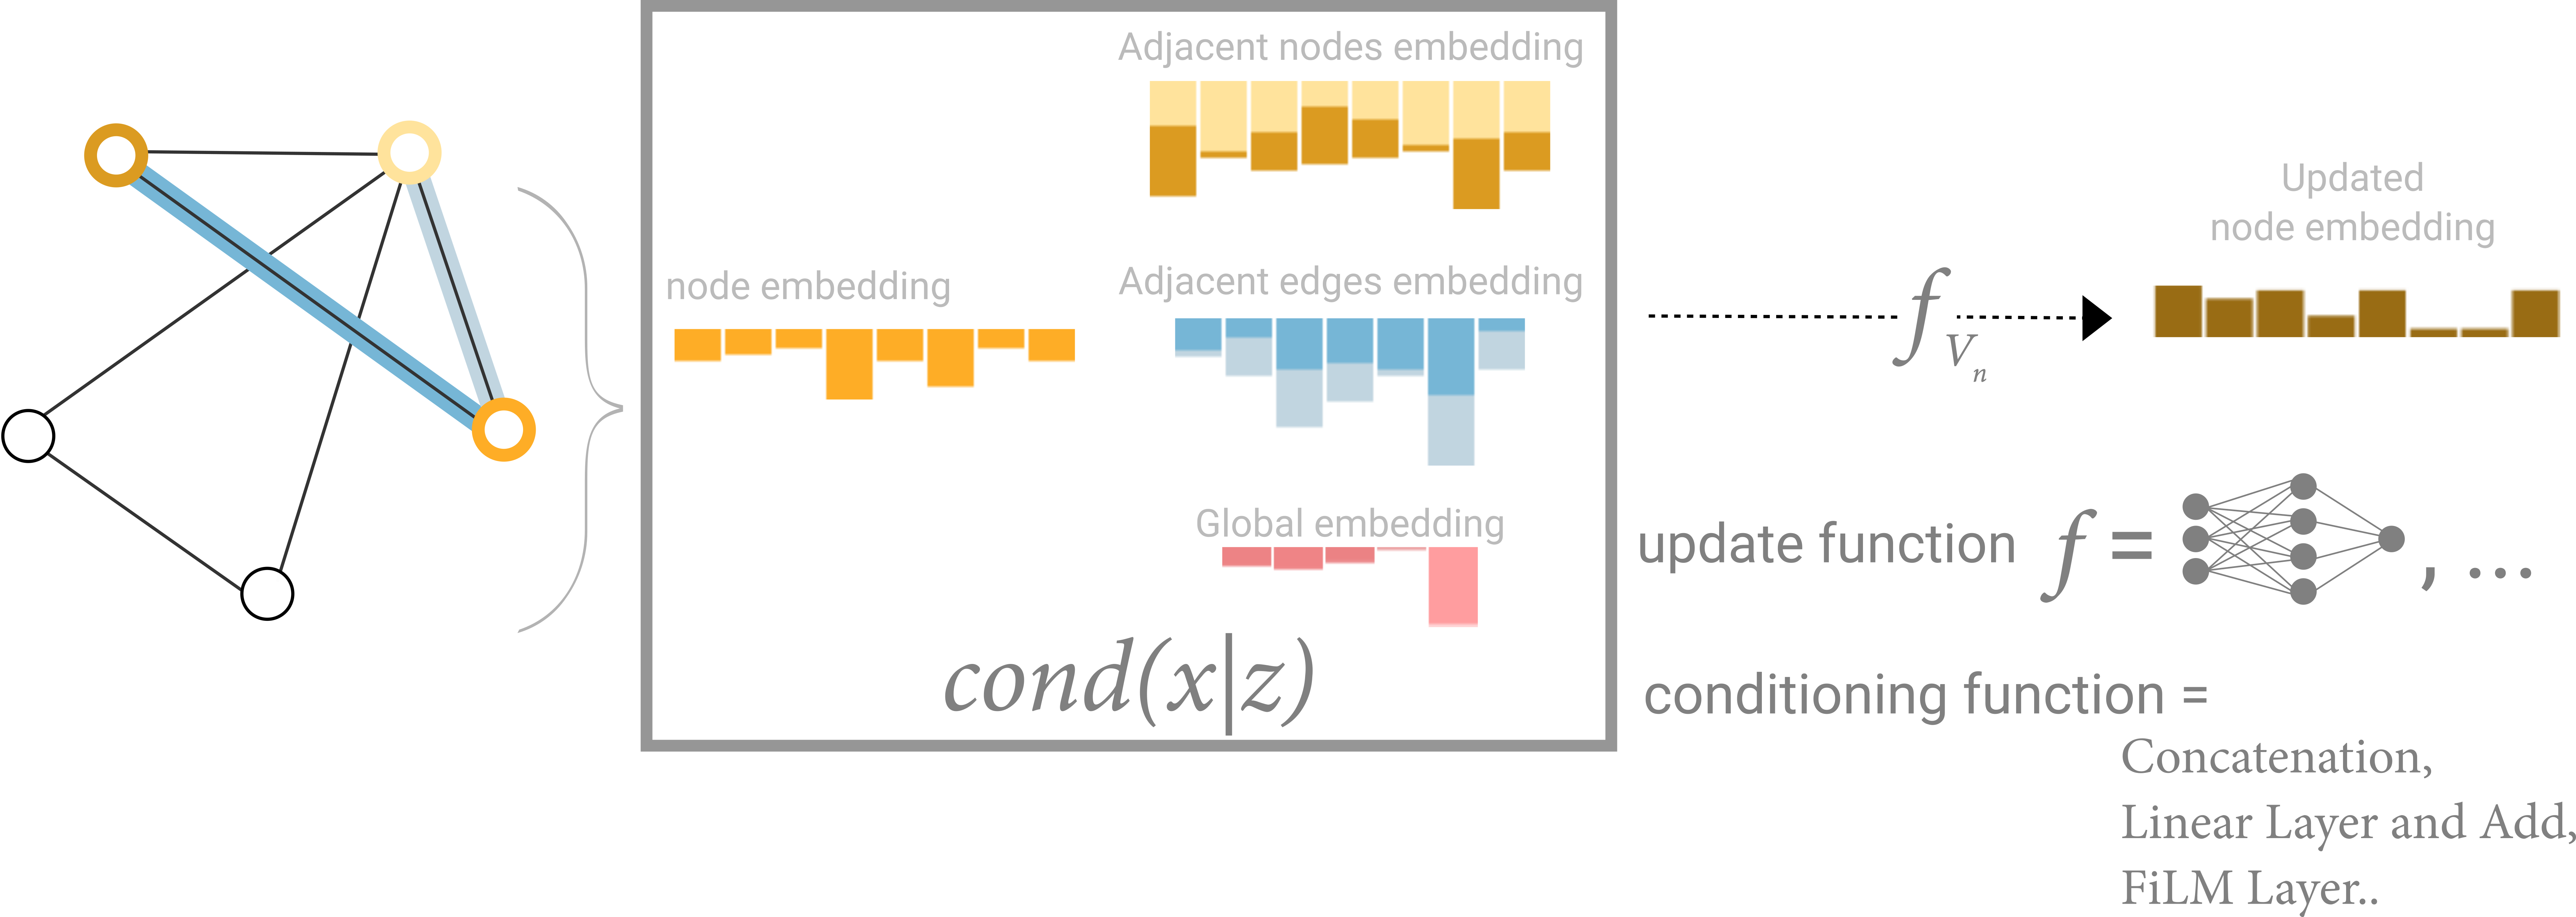
\includegraphics[width=.8\textwidth]{Images/conditioning-schematic.png}
    \end{figure}}
\end{frame}
%------------------------------------------------
\section{Into the Weeds}

%------------------------------------------------
\subsection{Other types of graphs}
\begin{frame}{}
    
\end{frame}
%------------------------------------------------

%---------------------------------------------------------
%	CLOSING SLIDE
%---------------------------------------------------------

% To remove miniframe from top
\appendix
\setbeamertemplate{headline}{}
\addtobeamertemplate{frametitle}{\vspace*{-\headheight}}{}

%---------------------------------------------------------
%	REFERENCES
%---------------------------------------------------------

\begin{frame}[noframenumbering, allowframebreaks] 
        \frametitle{References}

        \printbibliography
\end{frame}

%------------------------------------------------

\end{document} 